\documentclass[11pt]{article}

\usepackage{comment} % enables the use of multi-line comments (\ifx \fi) 
\usepackage[a4paper,margin=1cm]{geometry}
\usepackage[utf8]{inputenc}
\usepackage[ngerman]{isodate}
\usepackage{gensymb}
\usepackage{graphicx}
\usepackage{booktabs}% http://ctan.org/pkg/booktabs
\usepackage{makecell}
\usepackage{tabularx}
\usepackage{ltablex}
\usepackage[x11names]{xcolor}
\usepackage{amsmath}
\usepackage{amssymb}
\usepackage{array}
\usepackage{wrapfig}
\usepackage{subcaption}
\usepackage{csquotes}
\usepackage{lscape}
\usepackage{afterpage}
\usepackage{listingsutf8}
\usepackage{geometry}
\usepackage{chngcntr}
\usepackage{multicol}
\usepackage{xcolor}
\usepackage{pifont}
\usepackage{outlines}
\usepackage{breqn}
\usepackage{textcomp}
\usepackage{bm}
\usepackage{enumitem}
\usepackage{hyperref}
\usepackage{mdframed}
\usepackage{scalerel}
\usepackage{stackengine}
\usepackage{mathtools}
\usepackage{pdfpages}

% Code highlighting
\usepackage{minted}
\surroundwithmdframed{minted}

% Be able to caption equations and float them in place
\usepackage{float}
\usepackage{caption}

\newmdtheoremenv{theorem}{Theorem}

\DeclareCaptionType{equ}[Equation][List of Equations]

\counterwithin{figure}{section}

\AtBeginDocument{\counterwithin{lstlisting}{section}}

\geometry{a4paper, margin=1in}

\renewcommand*{\thead}[1]{\bfseries #1}
\newcommand{\code}[1]{\texttt{#1}}
\def\doubleunderline#1{\underline{\underline{#1}}}

\def\imagetop#1{\vtop{\null\hbox{#1}}}

\newcommand\equalhat{\mathrel{\stackon[1.5pt]{=}{\stretchto{%
    \scalerel*[\widthof{=}]{\wedge}{\rule{1ex}{3ex}}}{0.5ex}}}}

\newcommand\defeq{\mathrel{\overset{\makebox[0pt]{\mbox{\normalfont\tiny def}}}{=}}}

\newcolumntype{C}{>{\centering\arraybackslash}X}

\DeclarePairedDelimiter\abs{\lvert}{\rvert}
\DeclarePairedDelimiter\norm{\lVert}{\rVert}


\definecolor{lightgray}{rgb}{.9,.9,.9}
\definecolor{darkgray}{rgb}{.4,.4,.4}
\definecolor{purple}{rgb}{0.65, 0.12, 0.82}
\definecolor{darkgreen}{rgb}{0.05,0.56,0.06}
\definecolor{mauve}{rgb}{0.8863,0.5216,1}

\setcounter{tocdepth}{3}
\setcounter{secnumdepth}{3}

\graphicspath{{./img/}}



\begin{document}

\title{Deep Learning HS19}
\author{Pascal Baumann\\pascal.baumann@stud.hslu.ch}
\maketitle

For errors or improvement raise an issue or make a pull request on the \href{https://github.com/KilnOfTheSecondFlame/mse_summaries}{github repository}.

\tableofcontents

\newpage

\section{Introduction}
Deep Learning is a sub-branch of Machine Learning. Machine Learning itself is at the convergence point of Mathematics, Algorithmics, Optimization, Signal Processing and Software Engineering, and "could be defined as a set of methods that automatically detect patterns in data, and then use the uncovered patterns to predict future data, or to perform other kinds of decision making under uncertainty."

\begin{figure}[hbt]
	\centering
	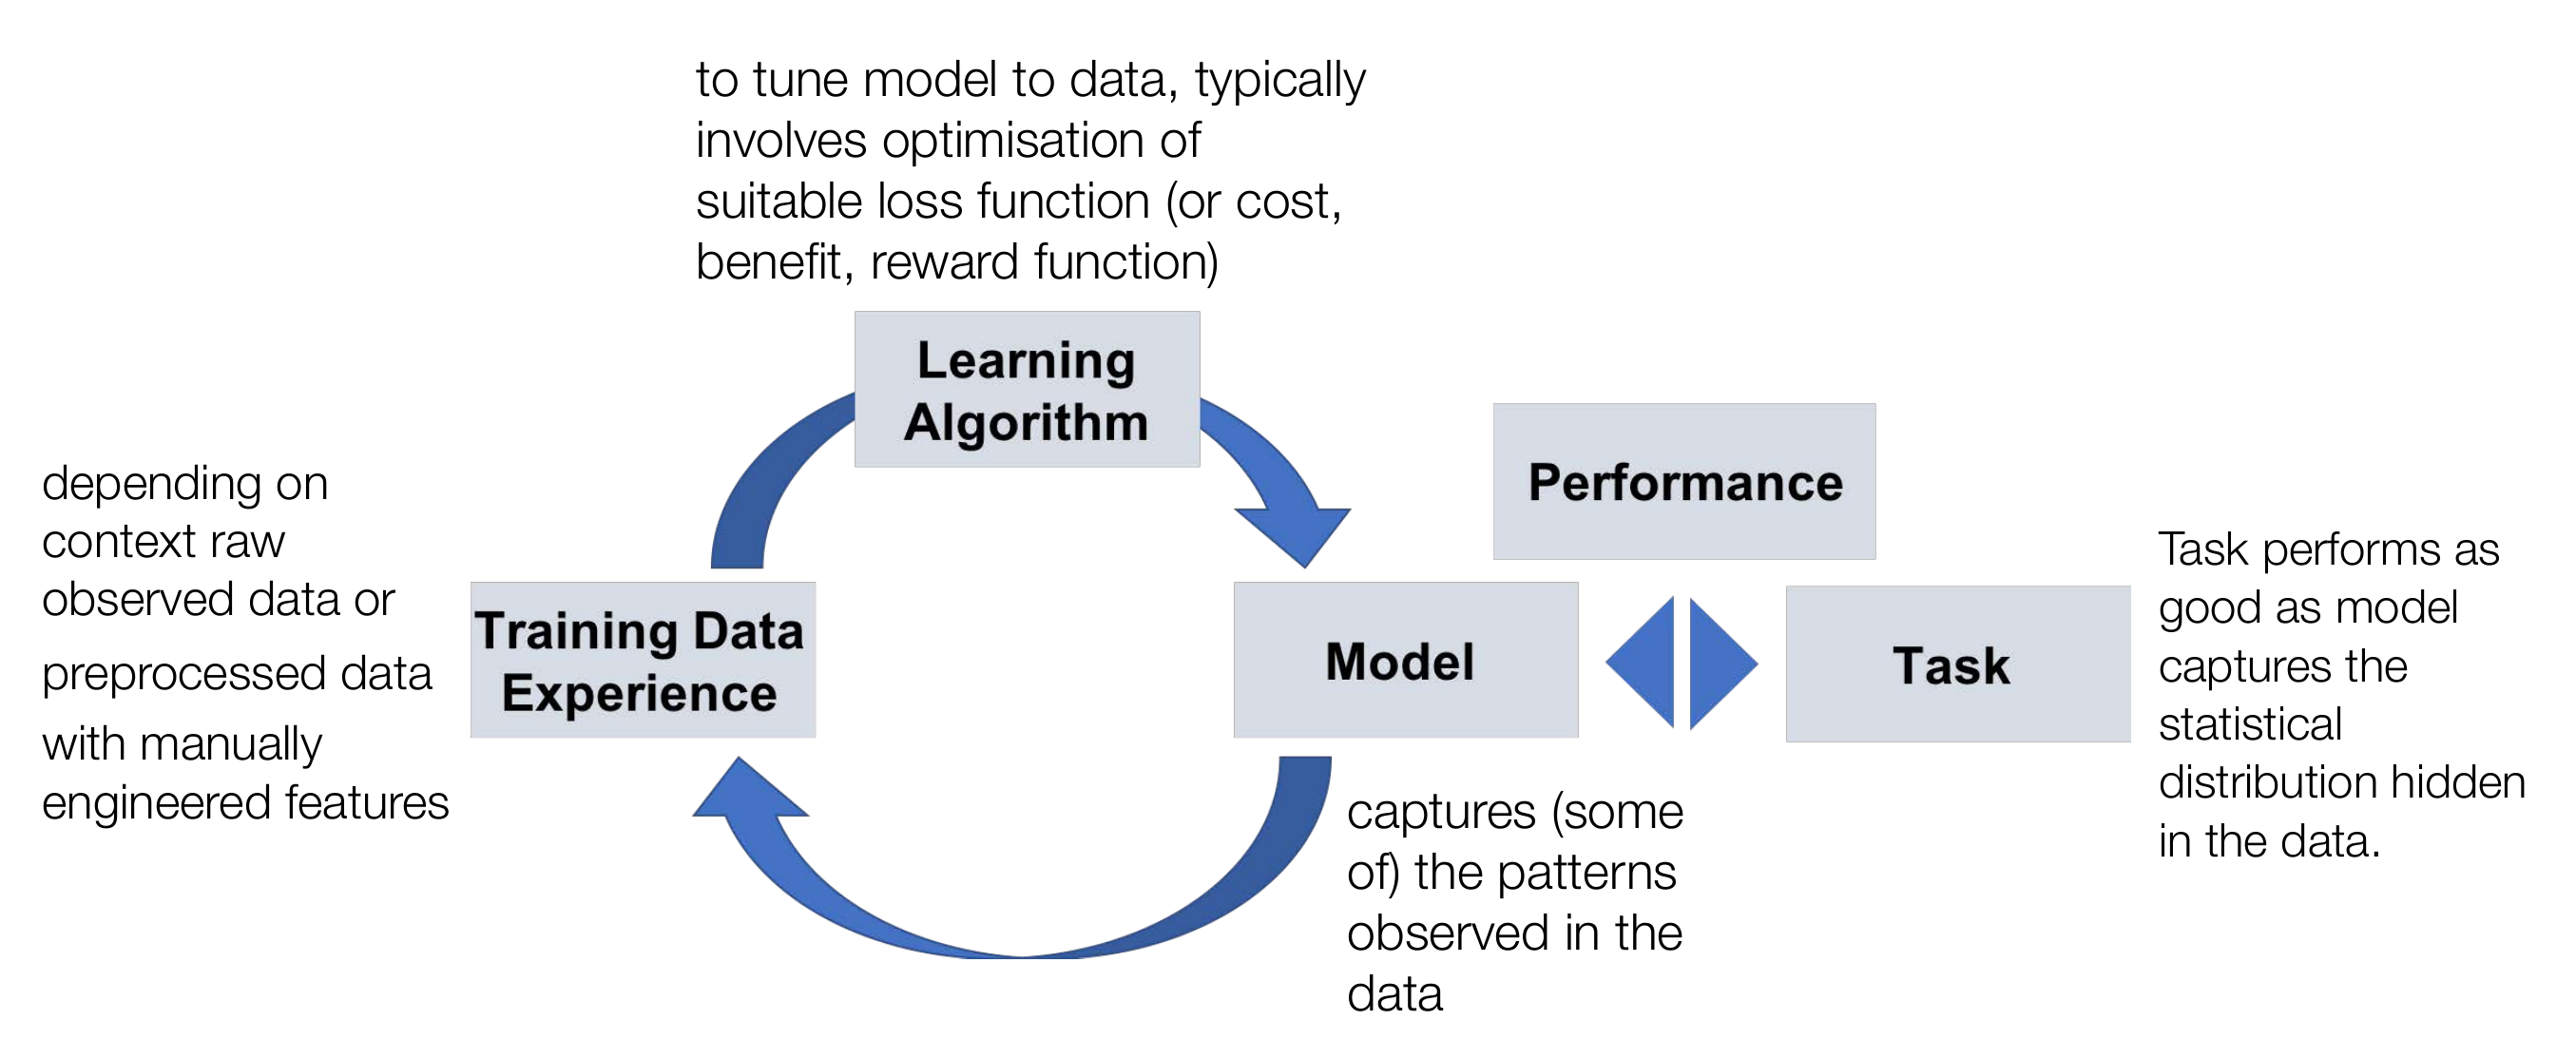
\includegraphics[width=0.8\linewidth, keepaspectratio]{img/machine_learning_overview}
	\caption{An overview of the Machine Learning workflow}
	\label{fig:machinelearningoverview}
\end{figure}

When talking about Machine Learning there is a distinction between \textbf{supervised learning} and \textbf{unsupervised learning}. In supervised learning the goal is to extract some relevant features x from raw observation data o and to learn a mapping from inputs x to outputs y given a set of example data called the training set.

In contrast to unsupervised learning where the goal is to discover interesting structures from inputs x given a set of data called the training set. Or in other words, to determine characteristics or features that can be used to optimally define groups.

\begin{figure}[hbt]
	\centering
	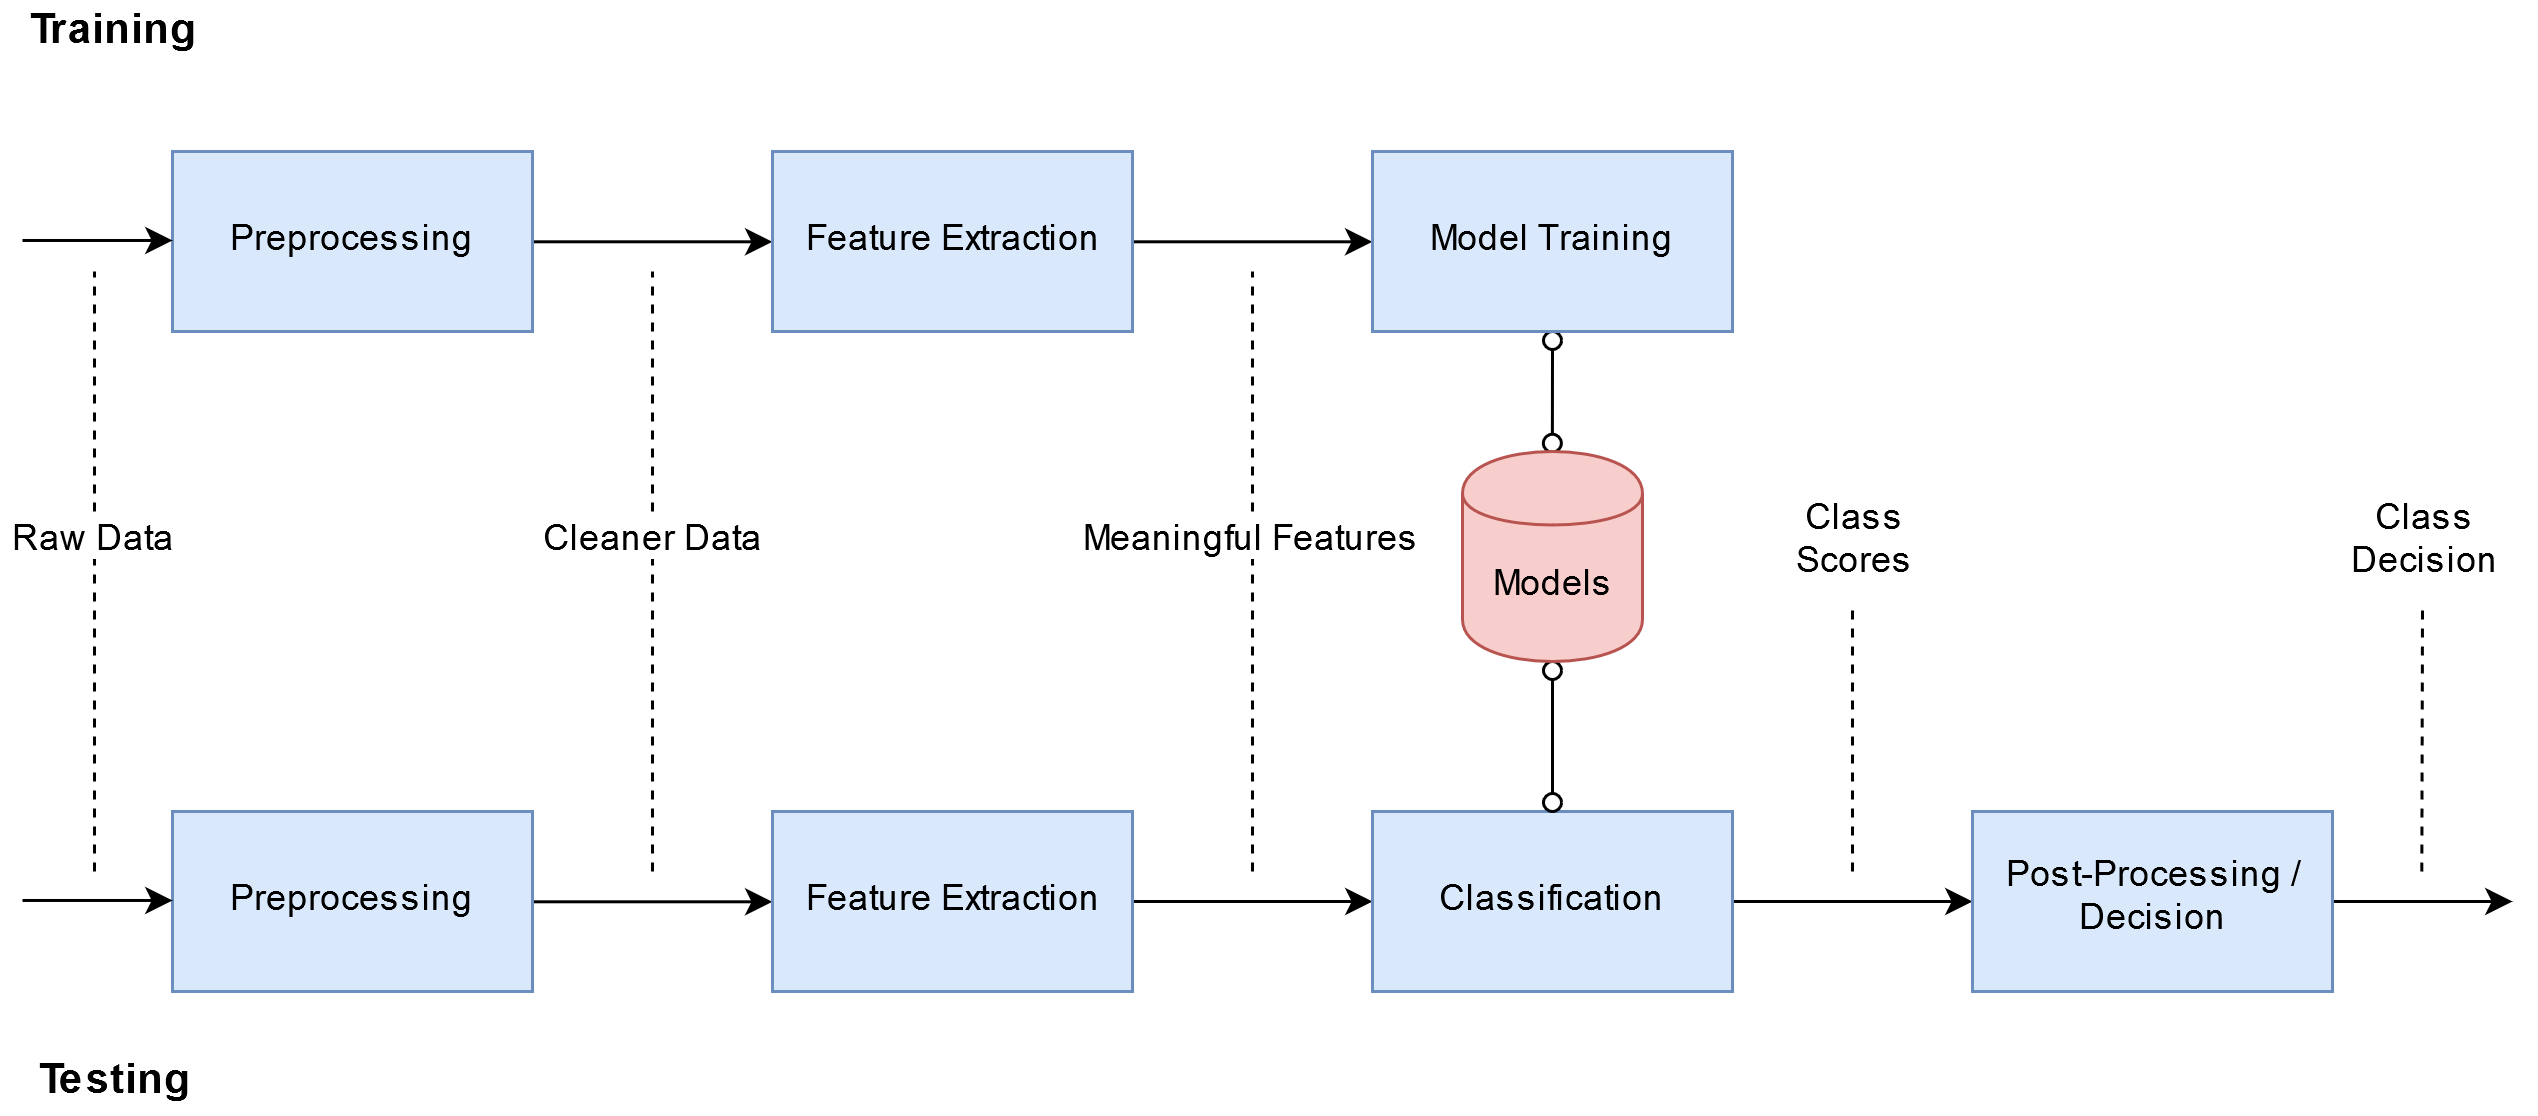
\includegraphics[width=0.8\linewidth, keepaspectratio]{img/machine_learning_process}
	\caption{The machine learning process}
	\label{fig:machinelearningprocess}
\end{figure}

As mentioned before, Deep Learning is a new subfield of Machine learning and at the convergence of larger quantities of data, new algorithms and better computer performance, even specialised computers for machine learning. In the core deep learning is a neuronal architecture with many layers and neurons, where less or no feature extraction is needed, as the model finds them automatically as part of the learning. The drawback is, that Deep Learning models need much more data than Machine Learning models.

\section{Perceptron}

The neuron in artificial neural networks is modelled after a neuron of the human brain, as it is able to send a signal after receiving enough activations until his own threshold is reached. The first artificial neuron model was the McCulloch-Pitts Neuron visualised in \ref{fig:mccullochpittsneuron}. They showed that, in principle, any logical or arithmetic function can be computed with networks of such neurons.

\begin{figure}[hbt]
	\centering
	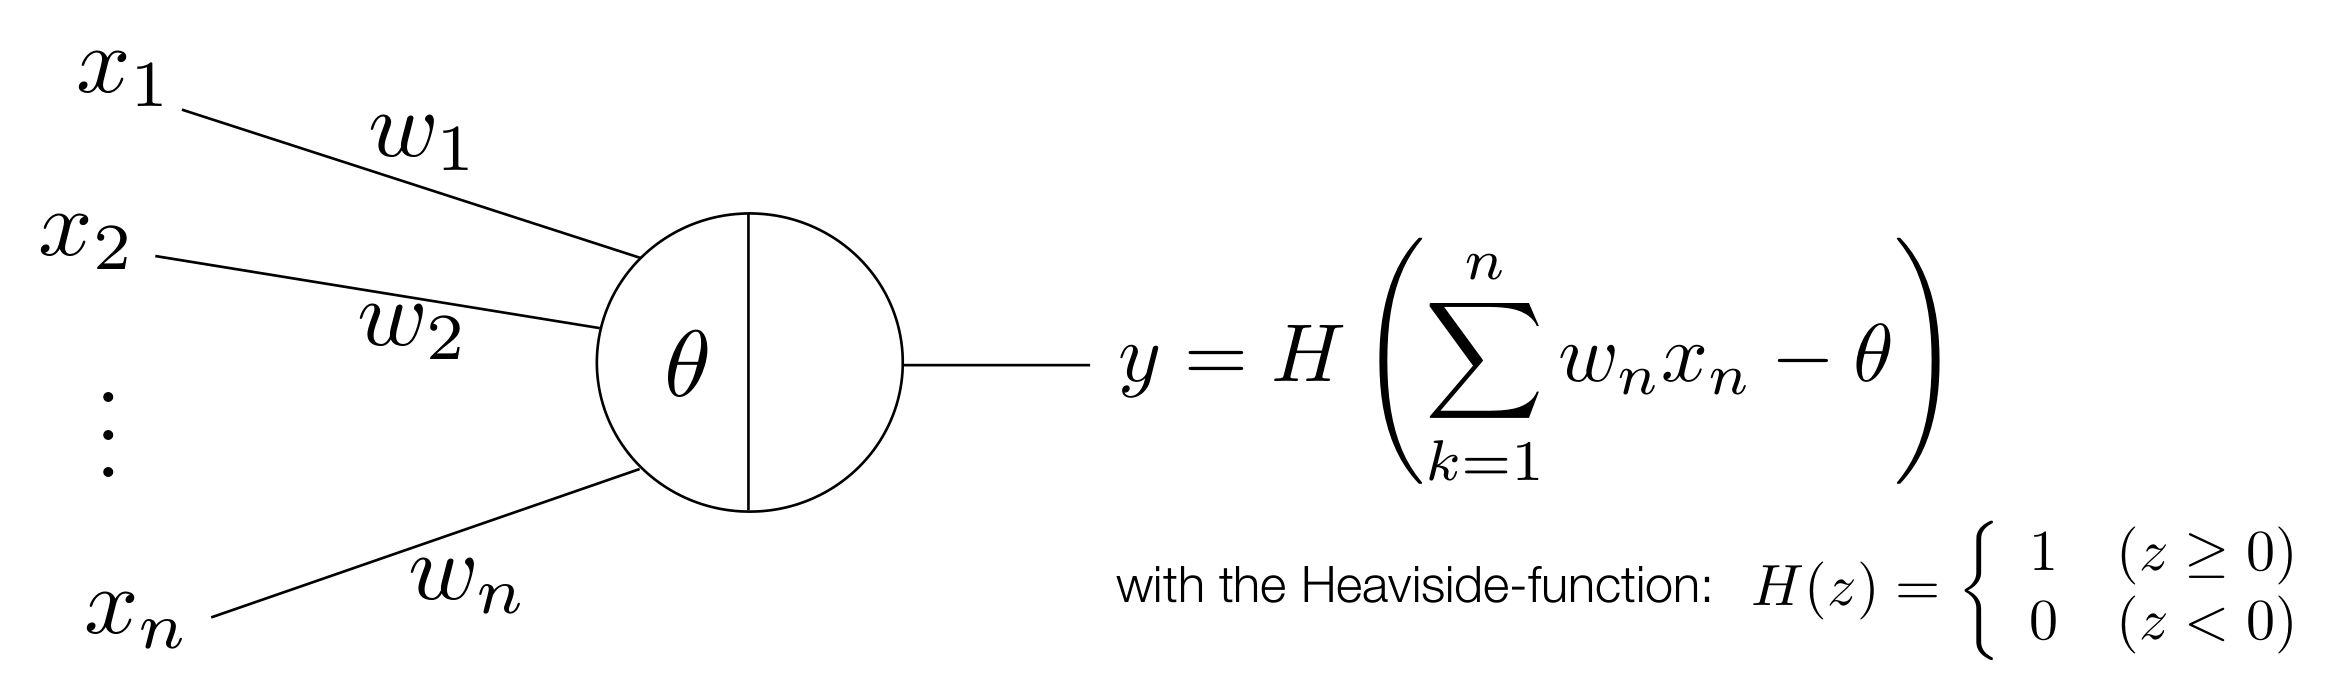
\includegraphics[width=0.8\linewidth, keepaspectratio]{img/mcculloch_pitts_neuron}
	\caption{McCulloch-Pitts Neuron}
	\label{fig:mccullochpittsneuron}
\end{figure}

In 1949 Donald Hebb postulated what is now known as Hebb's Rule:
"Let us assume that the persistence or repetition of a reverberatory activity tends to induce lasting cellular changes that add to its stability. [...] When an axon of cell A is near enough to excite a cell B and repeatedly or persistently takes part in firing it, some growth process or metabolic change takes place in one or both cells such that A's efficiency, as one of the cells firing B, is increased."
This hypothesis is not proven biologically, but is taken as a principle for ANNs to adjust their connection weights. It should be noted, however, that this learning rule does not provide a stable learning.

In 1958 Rosenblatt presented a single perceptron, also referred as Linear Threshold Unit (LTU):

\begin{itemize}
	\item Inputs and outputs are \emph{real numbers}
	\item Each input connection is associated with a \emph{real} weight
	\item The activity is computed by applying the Heaviside function to the weighted sum of the input while incorporating the activation threshold in form of a bias term $b$
	\begin{equation*}
		y = H\left(\sum_{k=1}^{n} w_k x_k + b \right)\quad\text{for } x_k,w_k,b\in\mathbb{R}
	\end{equation*}
	Thus the output can take on two distinct values {0,1}
\end{itemize}

\begin{equ}[H]
	\begin{equation*}
		H(x) = \left\{\begin{matrix}
			0 & x<0\\
			1 & x\geq 0
		\end{matrix}\right.
	\end{equation*}
	\caption{The Heaviside step function}
\end{equ}

A single perceptron can be used for binary classification problems, where the decision boundary is given by

\begin{equation*}
	H_{w,b} = \left\{ \textbf{x} \in \mathbb{R}^D | \textbf{w} \cdot \textbf{x} + b = 0 \right\}\quad\text{with }\textbf{w}=\begin{pmatrix}
		w_1\\
		\vdots\\
		w_D
	\end{pmatrix},
	\textbf{x} = \begin{pmatrix}
	x_1\\
	\vdots\\
	x_D
	\end{pmatrix}
\end{equation*}

Therefore the perceptron is suited for \textbf{linearly separable binary classification problems}.

\begin{figure}[hbt]
	\centering
	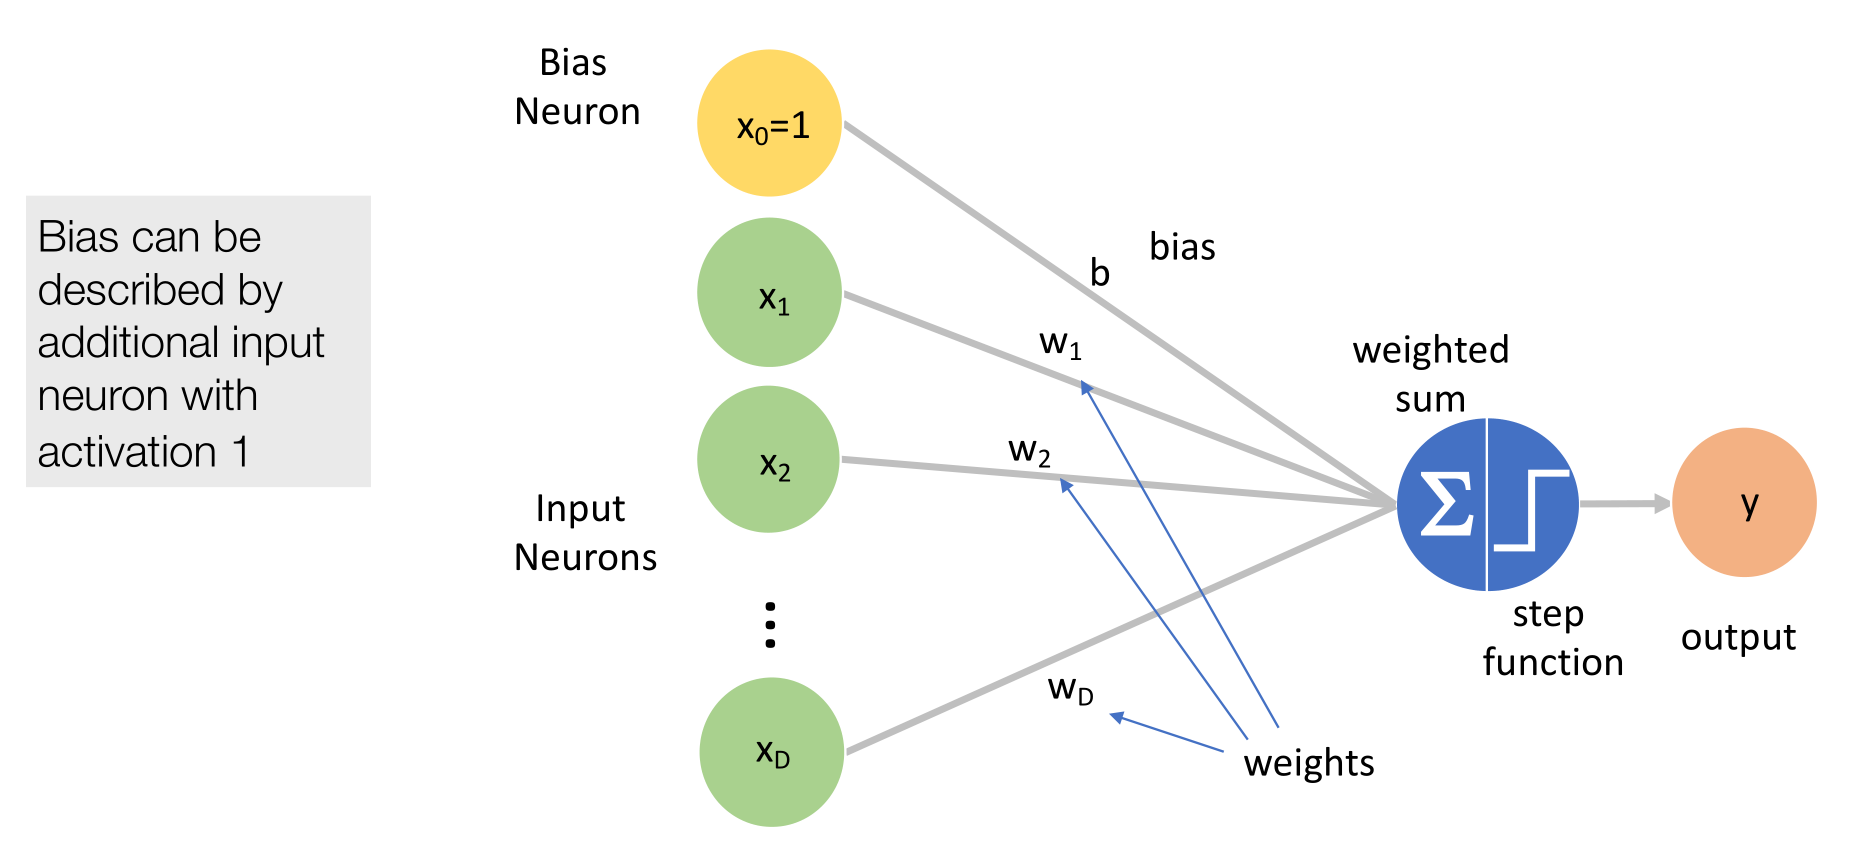
\includegraphics[width=0.6\linewidth, keepaspectratio]{img/rosenblatt_perceptron}
	\caption{The Rosenblatt perceptron}
	\label{fig:rosenblattperceptron}
\end{figure}

\subsection{Perceptron Learning Algorithm}
Labelled Data: \qquad ${(\textbf{x}^{(i)},y^{(i)})|i=1,...,N}$ where $\textbf{x}^{(i)}$ are $d$-vectors
\begin{enumerate}
	\item Initialise parameters\\
	all zeroes or small random numbers
	\item Iterate by updating weights according to
		\begin{enumerate}[label=\Alph*.]
			\item Pick sample \qquad\qquad\qquad\qquad$\left( \textbf{x}^{(i)},y^{(i)} \right)$
			\item Compute predicted values \qquad $\hat{y}^{(i)} = H(\textbf{w}\cdot\textbf{x}^{(i)} + b)$
			\item Parameter update rule \quad\quad\quad only update if $\hat{y}^{(i)} \ne y^{(i)}$\\
			\begin{align*}
				\textbf{w} &\leftarrow \textbf{w} - \alpha \cdot \left(\hat{y}^{(i)} - y^{(i)}\right) \cdot \textbf{x}^{(i)}\\
				b &\leftarrow b - \alpha \cdot \underbrace{\left(\hat{y}^{(i)} - y^{(i)}\right)}_{{-1,0,1}}
			\end{align*}
		\end{enumerate}
\end{enumerate}

The learning rule searches for a weights vector that defines a hyperplane that separates the points associated with the two classes. This is only possible for linearly separable input sets. In case of wrongly classified points, the weights update rule leads to a correction of the weights such that the hyperplane is tilted to try to bring the wrongly classified points to the correct side.

\begin{theorem}
	Perceptron Learning Algorithm converges in a finite number of steps to a weights vector and bias that separates the two classes - provided that the two classes are linearly separable.
\end{theorem}

However, the solutions obtained for linearly separable inputs is not unique and not optimal. The optimal solution (with the widest separating corridor) is known as the linear support vector machine (SVM). The perceptron may be a reasonable model also for problems that are not linearly separable. However, the application of the Perceptron Learning Algorithm does not converge in this case.

\subsection{Single Layer LTUs}
The inputs for ANNs are often represented using special \emph{passthrough} neurons called \textbf{input neurons}, if each neuron in the subsequent layer is connected to all the preceding neurons, the layer is \textbf{fully connected}. Generally, an extra bias feature $x_0 = 1$ is added, often represented with a \textbf{bias neuron} that just outputs one and whose influence is adjusted by the weight (see \ref{fig:rosenblattperceptron}).

\subsubsection{Possible Applications}
A single layer LTU with \emph{m} units can classify instances simultaneously into \textbf{\emph{m} different binary classes}, that is a multi-output classifier that can perform multiple tasks and is able to apply the learning algorithm independently to each output.

\begin{figure}[htb]
	\centering
	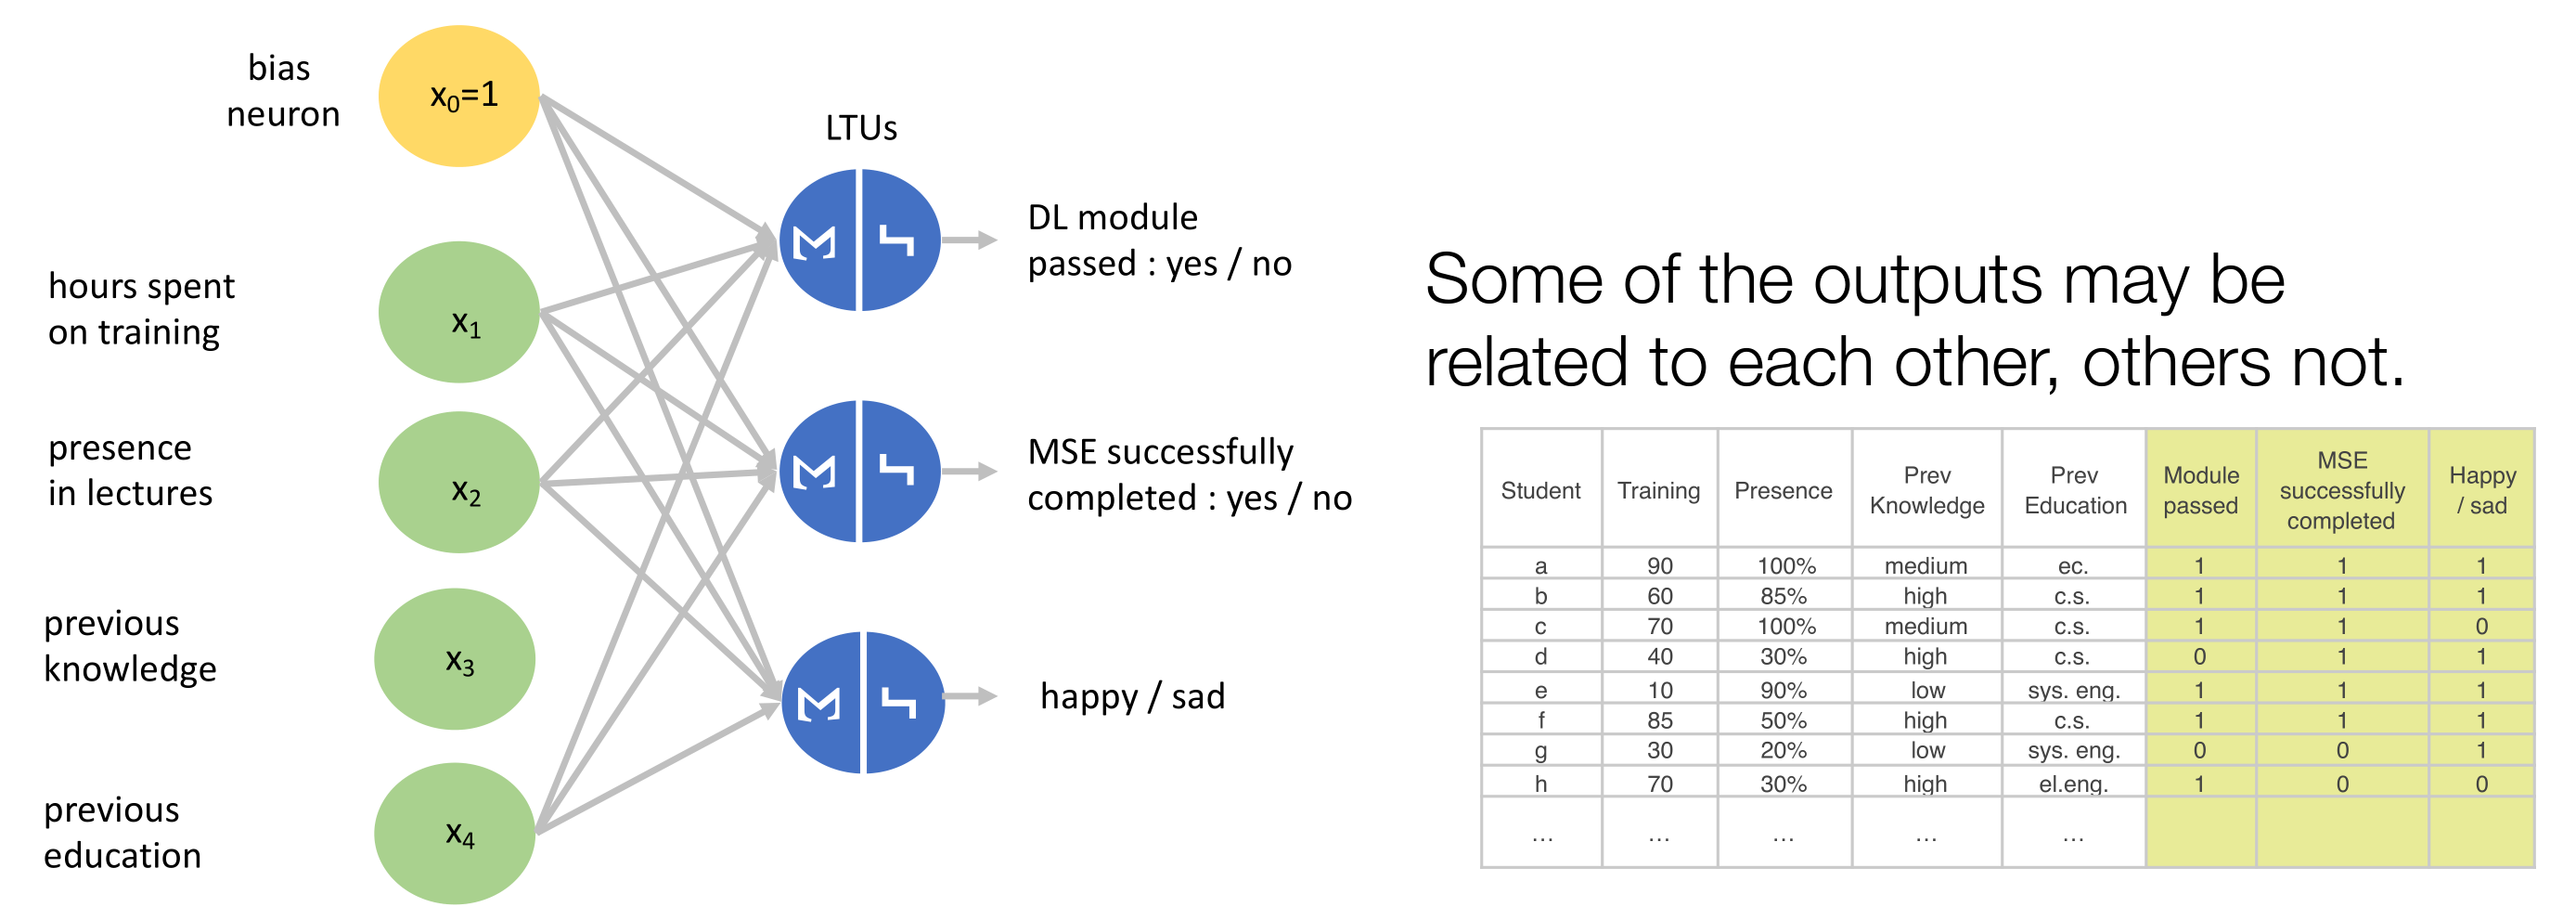
\includegraphics[width=0.8\linewidth, keepaspectratio]{img/multioutput_binary_classifier}
	\caption{An example for a multi-output classification with LTU}
	\label{fig:multioutputbinaryclassifier}
\end{figure}

The same model might also be considered for classifying input data into \emph{m} different exclusive classes. The output values, or labels, in the dataset would be prepared as one-hot vectors with only one non-zero entry. There are better ways for handling this task, like the Softmax algorithm, which will be introduced in a future section.

\begin{figure}[htb]
	\centering
	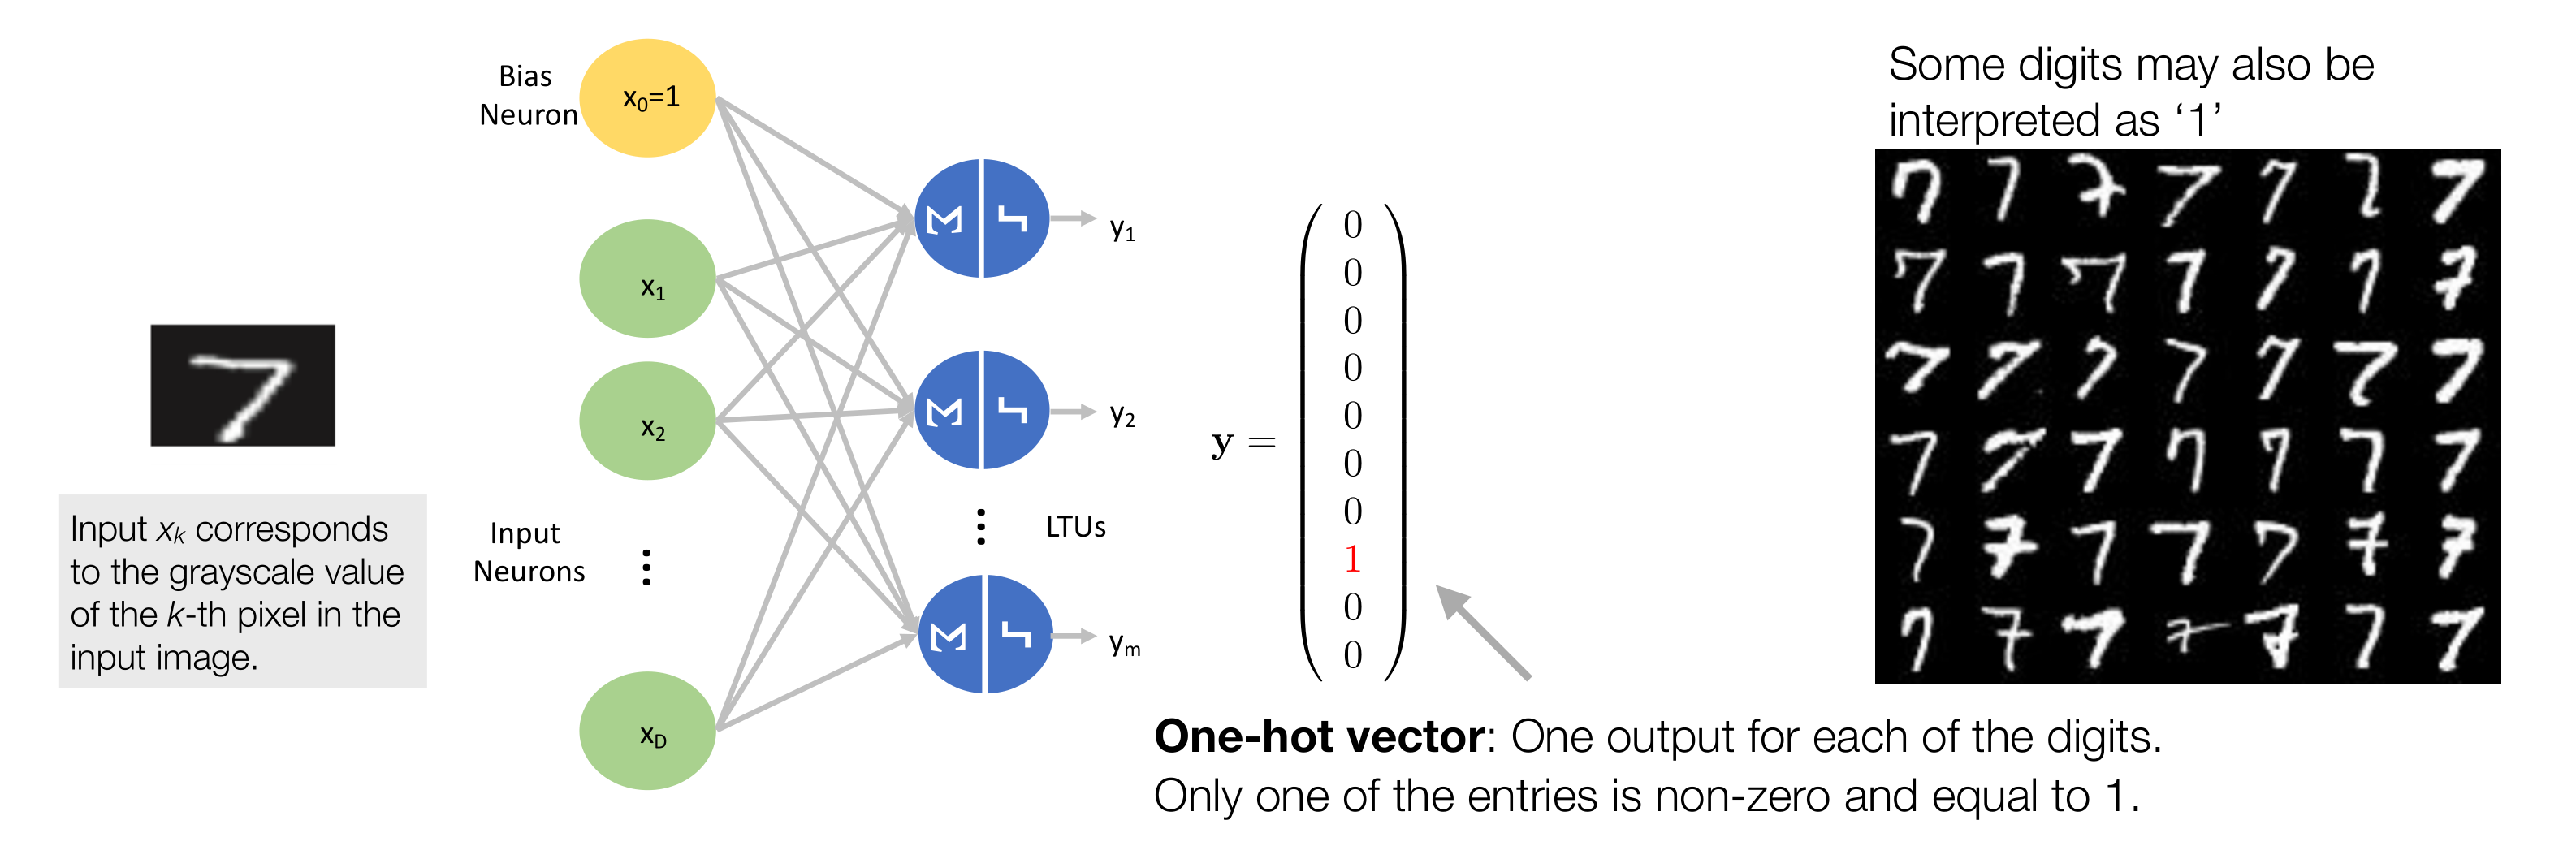
\includegraphics[width=0.8\linewidth, keepaspectratio]{img/exclusive_multioutput_classifier_ltu}
	\caption{An example for an exclusive multi-output classification with LTU}
	\label{fig:exclusivemultioutputbinaryclassifier}
\end{figure}

\begin{minipage}{0.5\textwidth}
	The limitation of a single layer perceptron is that it's incapable of solving problems with a non-linear decision boundary. This limitation can be overcome by stacking multiple layers of a perceptron into a so called Multi-Layer Perceptron (MLP). An MLP is composed of:
	\begin{itemize}[label=-]
		\item Input layer: Inputs are passed by pass-through neurons
		\item Hidden layers: One or more layers of LTUs
		\item Output layer: Final layer with a single or multiple LTUs (depending on the problem)
	\end{itemize}
\end{minipage}
\begin{minipage}{0.5\textwidth}
	\centering
	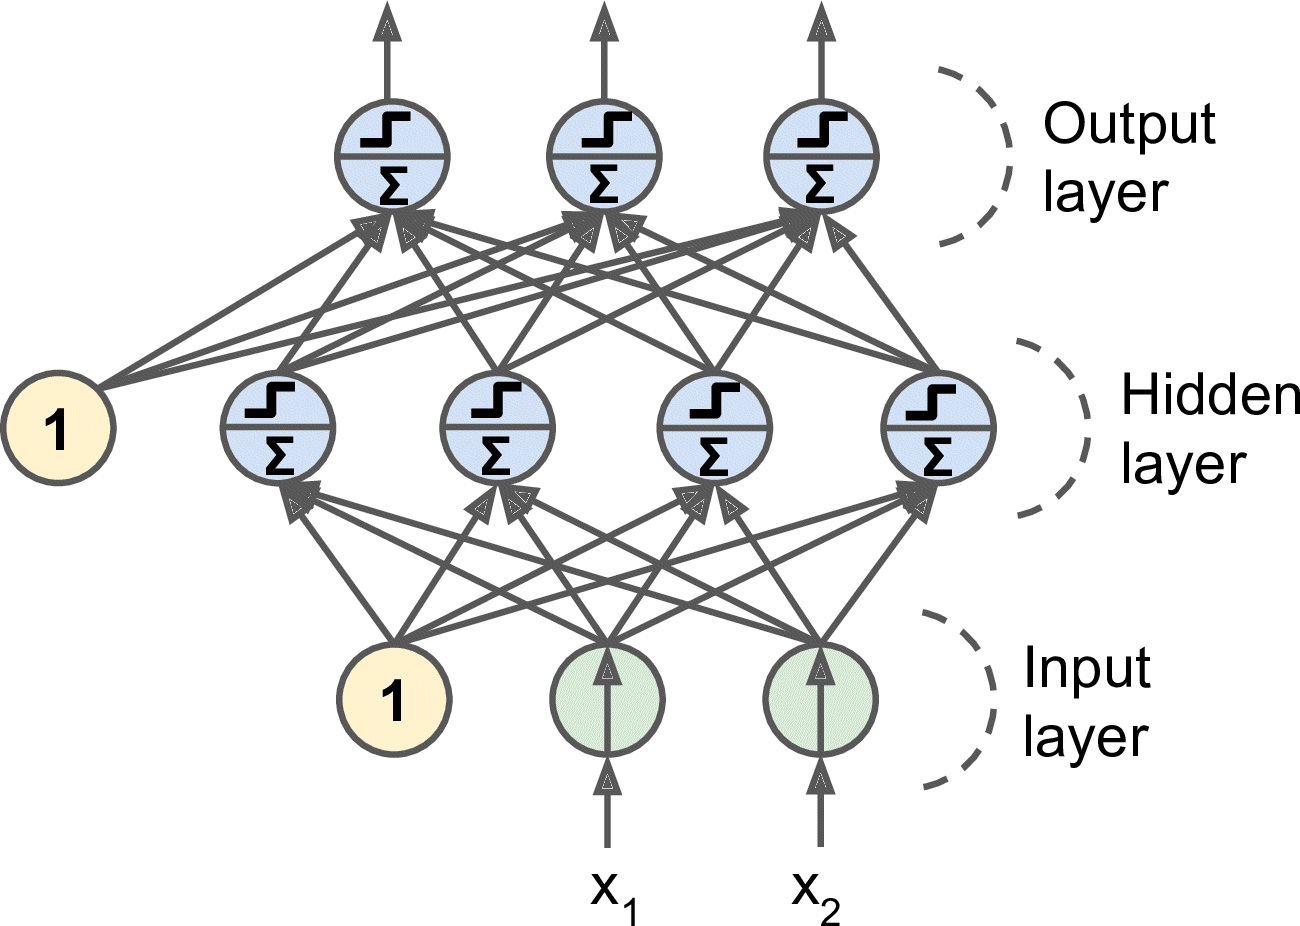
\includegraphics[width=0.9\linewidth, keepaspectratio]{img/multi_layer_perceptron}
\end{minipage}

Both the input layer and hidden layers of an MLP include a bias neuron, and are fully connected to the next layer. The Activation Function is a generalisation of the hard threshold (Heaviside Function) and replaced by smooth functions.

\section{MNIST}
MNIST is a public dataset with labelled data widely used for testing and illustration:
\begin{itemize}[label=-]
	\item 70000 images
	\item 28x28-pixel
	\item available for download from \url{mldata.org}
\end{itemize}

\subsection{Load MNIST Images}

\begin{minted}[linenos]{python}
import tensorflow as tf
mnist = tf.keras.datasets.mnist
# load data and split into train and test set
(x_train, y_train),(x_test, y_test) = mnist.load_data()
# normalise data to lie between 0 and 1
x_train, x_test = x_train / 255.0, x_test / 255.0
\end{minted}

\section{Data Preparation}

\subsection{Training and Test Set}
Split the data into training and test set, making sure that both sets have the same characteristics. It's a good idea to randomly shuffle the datasets before splitting, unless one is sure that the dataset is already sufficiently shuffled. It's of utmost importance to keep the two sets strictly separate while training, so no information contained in the test set is used to adjust parameters of the model.

\begin{table}[h!]
	\centering
	\begin{tabular}{|c|c|c|}
		\hline
		&\textbf{Small Datasets}&\textbf{Large Datasets}\\
		\hline
		Train & 70-80\% & 99 \% \\
		\hline
		Test & 30-20\% & 1\%\\
		\hline
	\end{tabular}
	\caption{Recommended Train/Test split given a particular size of the dataset}
\end{table}

\subsubsection{Splitting using SciKit-Learn}

\begin{minted}[linenos]{python}
form sklearn.model_selection import train_test_split

x_train, x_test, y_train, y_test = \
	train_test_split(xdata, ydata, test_size=0.3, random_state=1)	
\end{minted}

\subsection{Data Normalisation and Feature Scaling}
The numeric values of features contained in the data may be on different scales, ranging over different order of magnitude or centred around different values on average. The data should thus be brought to similar scales, so called Feature Scaling, and approximately centred around zero, the so called Feature Centring. This is important as the \emph{numerical stability} of the learning algorithm depends on it and it can focus on learning the importance of the features, which leads to \emph{improved convergence properties}.

Two different methods are mostly used:
\begin{itemize}[label=-, noitemsep, nosep]
	\item z-Normalisation
	\item Min-Max-Rescaling or Min-Max Normalisation
\end{itemize}

\subsubsection{z-Normalisation}
\textbf{Shifting} and \textbf{rescaling} the data so that a zero mean and a unit-variance is obtained.
\begin{equation*}
	{x'}_k^{(i)} = \frac{x_k^{(i)}-\mu_k}{\sigma_k}
\end{equation*}
\noindent
where the mean and variance for the $k$-th component are
\begin{align*}
	\mu_k &= \frac{i}{N} \sum_{k=1}^{N}x_k^{(i)}\\
	\sigma_k^2 &= \frac{i}{N}\sum_{k=1}^{N}\left(x_k^{(i)}-\mu_k\right)^2
\end{align*}
\noindent
The parameters $\mu_k, \sigma_k$ should be \textbf{computed on the training set} only, as computing it on the whole data set is considered to falsify the training. When normalising image data the mean and standard deviation are calculated over all the pixels.

\subsubsection{Min-Max-Rescaling and Normalisation}
\paragraph{Min-Max-Rescaling}
\begin{equation*}
	{x'}_k^{(i)} = \frac{x_k^{(i)}-\text{min}_k}{\text{max}_k -\text{min}_k}
\end{equation*}
\noindent
Features are rescaled to lie in the $[0,1]$ range.

\paragraph{Min-Max-Normalisation}
\begin{equation*}
{x'}_k^{(i)} = 2\cdot\frac{x_k^{(i)}-\text{min}_k}{\text{max}_k -\text{min}_k} - 1
\end{equation*}
\noindent
Features are rescaled to lie in the $[-1,1]$ range.
\vspace{1em}
\noindent
The same remarks as for the z-Normalisation hold true: min/max should be computed on the training set, and computed over all pixels when using image data.

\section{Training a Model}

\subsection{Generalised Perceptron}

\begin{figure}[htb]
	\centering
	\begin{subfigure}[b]{0.3\textwidth}
		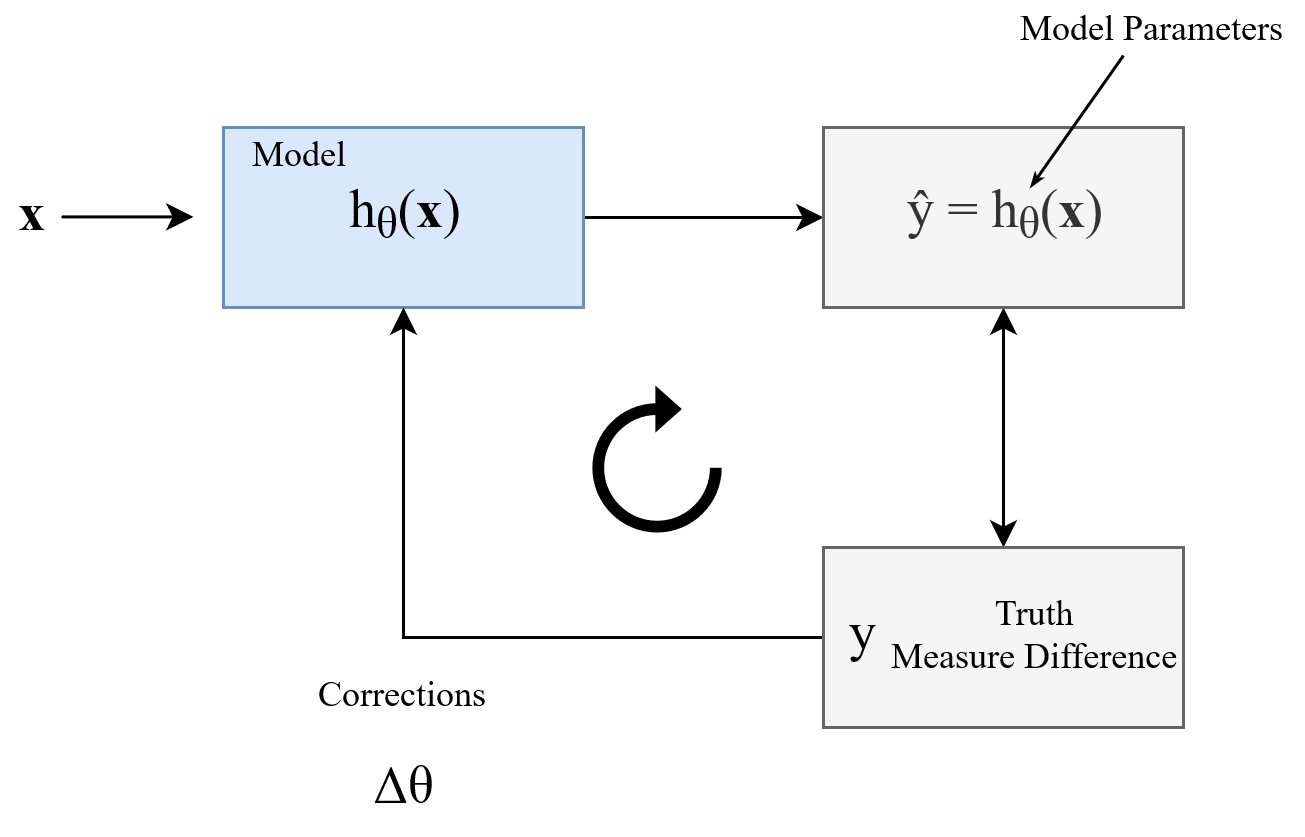
\includegraphics[width=\textwidth]{model_training}
		\caption{General training}
		\label{fig:generalmodeltraining}
	\end{subfigure}
	\begin{subfigure}[b]{0.3\textwidth}
		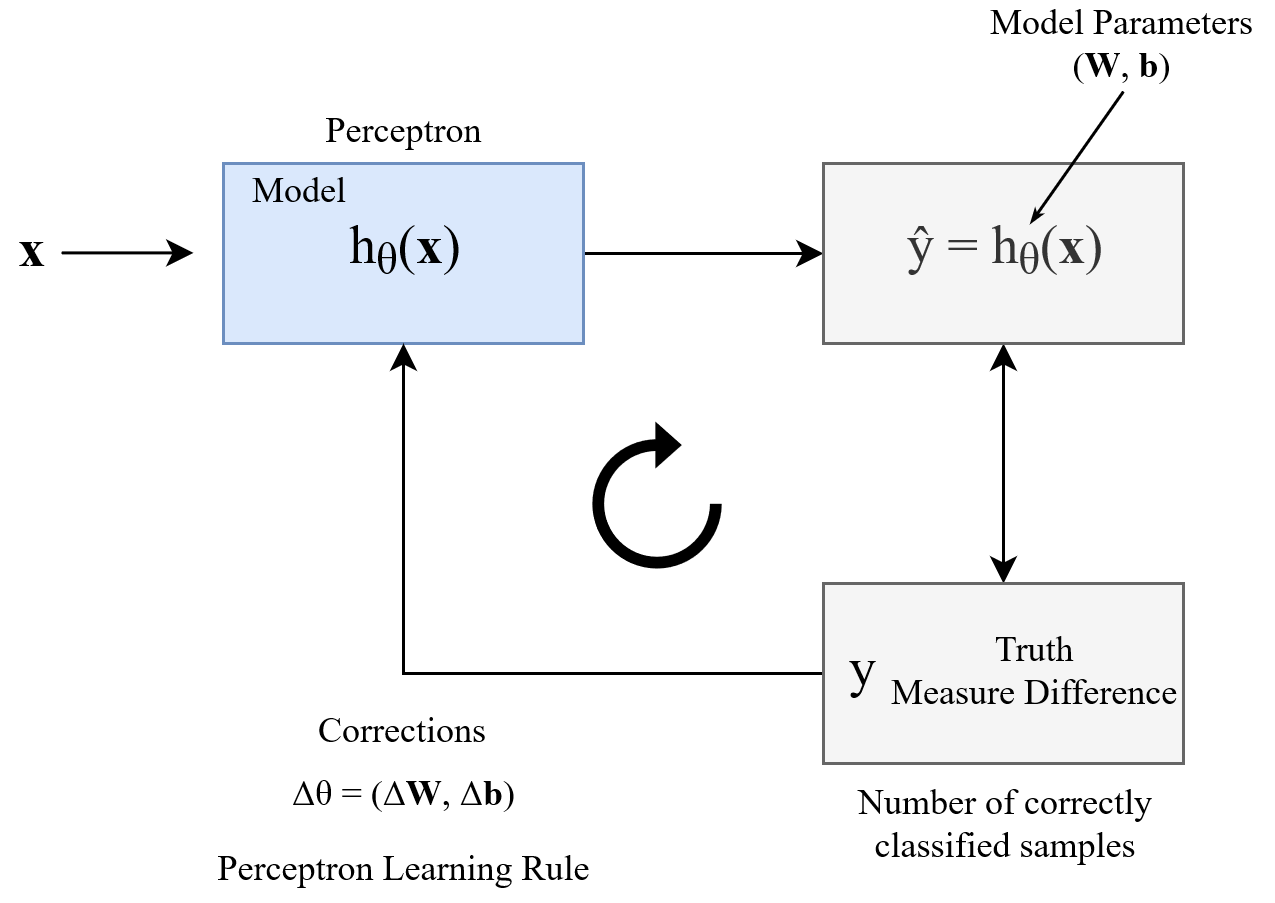
\includegraphics[width=\textwidth]{model_training_perceptron}
		\caption{Training a perceptron}
		\label{fig:perceptrontraining}
	\end{subfigure}
	\begin{subfigure}[b]{0.3\textwidth}
		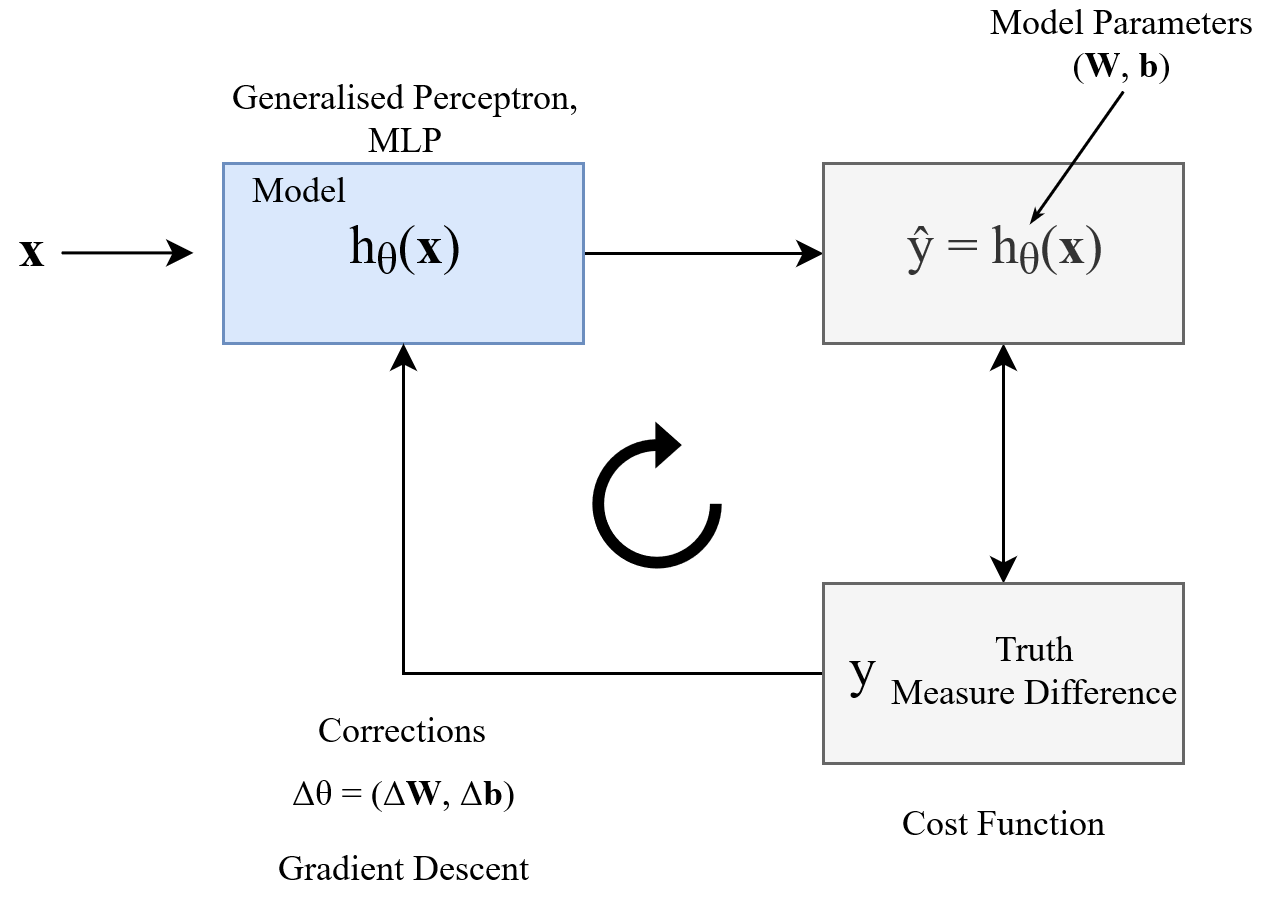
\includegraphics[width=\textwidth]{model_training_mlp}
		\caption{Training a MLP}
		\label{fig:mlptraining}
	\end{subfigure}
\end{figure}

The first generalisation from Rosenblatt's Perceptron is the replacement of the Heaviside function as the activation function through a smooth Sigmoid function:
\begin{equation*}
	\sigma(z) = \frac{1}{1+e^{-z}}
\end{equation*}
\noindent
This allows for a probabilistic interpretation of the output. The sigmoid is continuous and thus differentiable. With this, Optimisation techniques can be used.

The second generalisation is the use of the Optimisation technique Gradient Descent for Learning, this technique is also applicable for problems that are not linearly separable and for MLPs.

\subsubsection{Model for Binary MNIST Classification}

\begin{equation*}
	\hat{y} = h_\theta (\textbf{x}) = \sigma(\textbf{w}\cdot\textbf{x} + b)
\end{equation*}
\noindent
Where $\sigma(z)$ is the sigmoid function, and the model parameters $\theta =(\textbf{w}, b)$. The output is no longer binary, but a numeric value $\hat{y}\in\left]0,1\right[$ and can be transformed to a class label by the rule:
\begin{equation*}
	\hat{y} = \left\{ \begin{matrix}
		1 & \text{if } h_\theta(\textbf{x}) > 0.5\\
		0 & \text{if } h_\theta(\textbf{x}) \leq 0.5
		\end{matrix} \right.
\end{equation*}

\subsection{Cost Function}
Choose the initial parameters such that the predicted values $\hat{y}$ are in some notion of distance close to the true outcomes $y$. This notion of distance is expressed in terms of a cost function, whereas the parameters are chosen in such a way that this function is minimised. Different cost functions will lead to different solutions.

\subsubsection{Mean Square Error (MSE) Cost Function}
The MSE cost function is based on the principle of the mean quadratic distance between $y$ and $\hat{y}$.
\begin{equation}
	J_{\text{MSE}}(\theta) = \frac{1}{2m}\sum_{i=1}^{m}\left(h_\theta(x^{(i)})-y^{(i)}\right)^2
\end{equation}
\noindent
By minimising $J_{\text{MSE}}(\theta)$ with respect to the parameters $\theta$ we adjust the model to best represent the mapping $\textbf{x}\rightarrow y$ seen in the training data.

\subsubsection{Cross Entropy (CE) Cost Function}
The CE cost function is based on the Cross-Entropy Loss defined by

\begin{equation*}
	L_{\text{CE}}\left((\textbf{x},y\right),\theta) = -\log\left(p_\theta(y|\textbf{x})\right)
\end{equation*}

\noindent
\begin{minipage}[b]{0.5\linewidth}
	This loss function is suited for classification problems, and based on the model predicting the probability for observing class $y$ given $\textbf{x}$ denoted by $p_\theta(y|\textbf{x})$.
\end{minipage}
\begin{minipage}{0.5\linewidth}
	\centering
	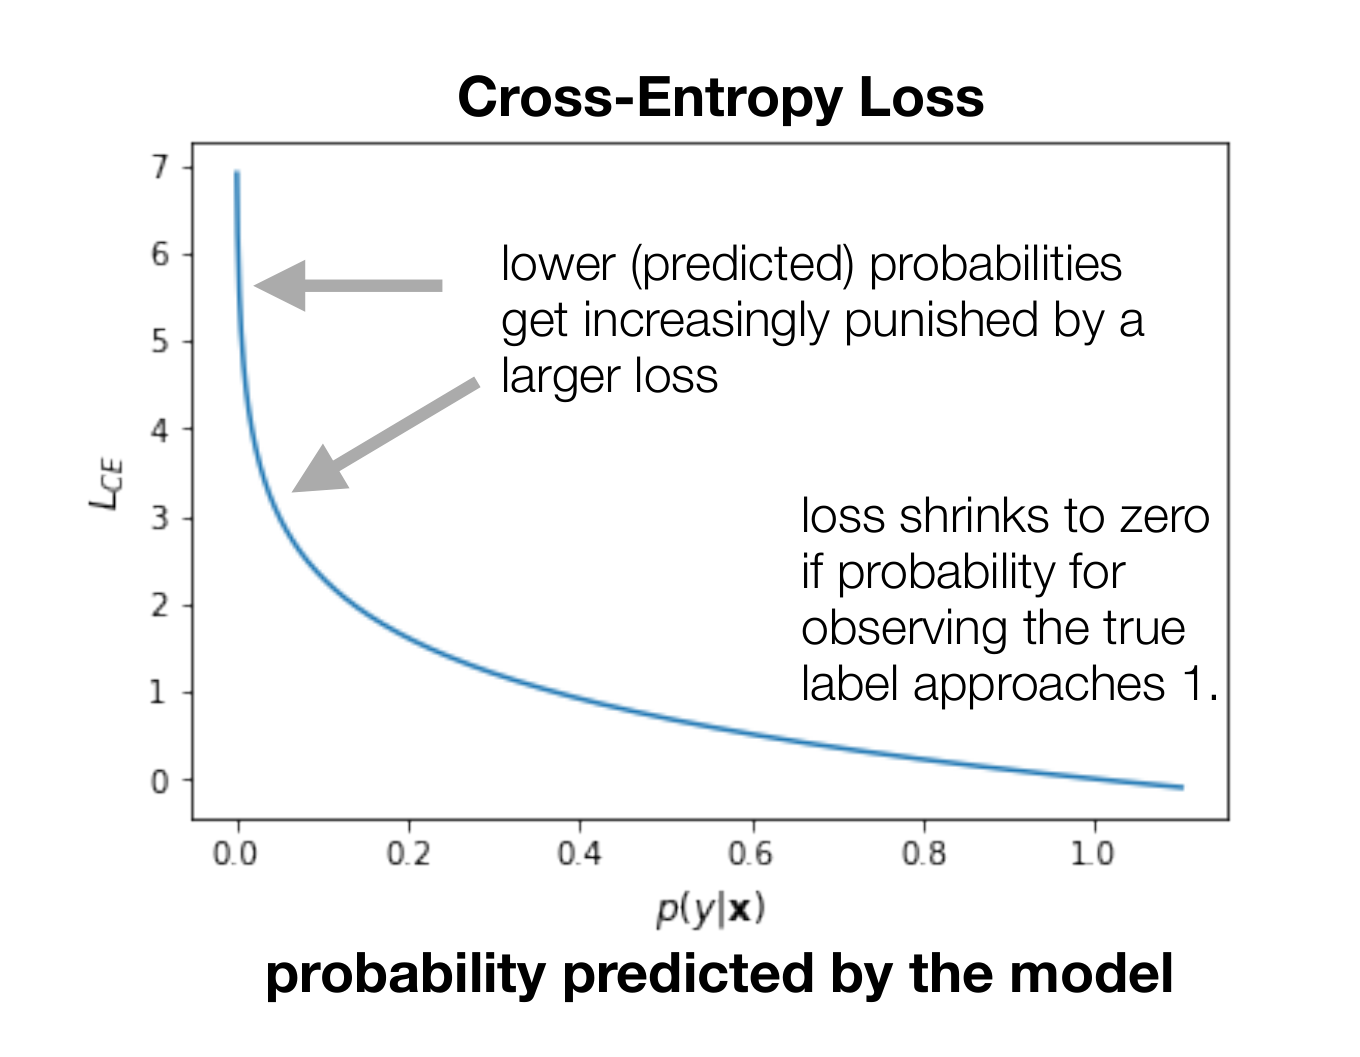
\includegraphics[width=0.8\linewidth, keepaspectratio]{img/cross_entropy_loss}
\end{minipage}

\noindent
The cross entropy cost function is then the averaged cross entropy loss
\begin{equation}
	J_{\text{CE}} = -\frac{1}{m} \sum_{i=1}^{m}\log\left(p\left(y^{(i)}|\textbf{x}^{(i)},\theta\right)\right)
\end{equation}

\noindent
For the binary classification problem
\begin{equation}
	J_{\text{CE}} = -\frac{1}{m} \sum_{i=1}^{m}\left( y^{(i)}\log(h_\theta(\textbf{x}^{(i)})) + (1-y^{(i)})log(1 - h_\theta(\textbf{x}^{(i)})) \right)
\end{equation}

\noindent
In the given single layer perceptron problem the cross-entropy cost function is a convex function. As a result, the function has a single local minimum (a single critical point) which is the global minimum. As long as the chosen learning rate is sufficiently small, the gradient descent will always converge to a global minimum.

\subsection{Gradient Descent}
The basic principle of the Gradient Descent is the minimisation of some cost function $J(\theta)$:
\begin{enumerate}
	\item Start with some initial value for the parameter vector: $\theta_0$
	\item Iteratively update the parameter vector by
	\begin{enumerate}[label=\roman*.]
		\item Compute the gradient of the cost function $J(\theta)$ at the last position reached ($\theta_t$)
		\item Step in the negative gradient direction according to
		\begin{equation*}
			\theta_{t+1} =\theta_t - \alpha \cdot\nabla_\theta J(\theta_t)
		\end{equation*}
		where $\alpha$ is the learning rate
	\end{enumerate}
	\item Stop when the change in parameter vector is small
\end{enumerate}

\begin{figure}[htb]
	\centering
	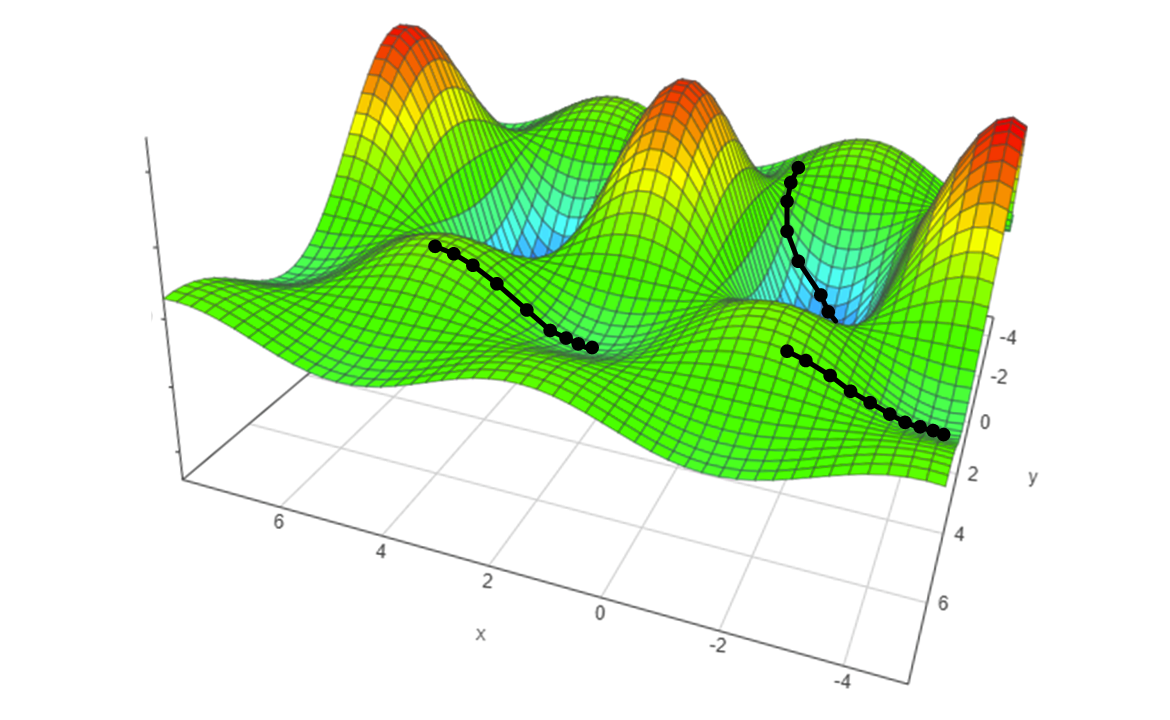
\includegraphics[width=0.6\linewidth, keepaspectratio]{img/gradient_descent}
	\caption{Illustration of a gradient descent, different initialisation and optimisers lead to different outcomes}
	\label{fig:gradientdescent}
\end{figure}

The learning principle works locally (by using local function properties and sufficiently small step sizes), but can get stuck in critical points were the gradient is zero. Without additional information the learning schema cannot discern between local minima, maxima or saddle point. Because the learning schema is iterative, it iteratively approaches a critical point and may fluctuate around it.

\subsubsection{Computing Gradients}

The Gradient is a \textbf{partial derivative} of the function $J(\theta) = J(\theta_1,\theta_2,...,\theta_n)$ with regard to $\theta_k$
\begin{equation*}
	\frac{\partial J}{\partial\theta_k} = \underset{\epsilon\rightarrow0}{\text{lim}}\left( J(\theta) = J(\theta_1,...,\theta_k+\Delta\theta_k,...,\theta_n) - J(\theta_1,...,\theta_k,...,\theta_n) \right)
\end{equation*}
\noindent
And the \textbf{gradient}:
\begin{equation*}
	\nabla_\theta J =\frac{\partial J}{\partial\theta} = \begin{pmatrix}
		\frac{\partial J}{\partial\theta_1}\\
		\vdots\\
		\frac{\partial J}{\partial\theta_n}
	\end{pmatrix}
\end{equation*}
\noindent
Linearisation (Taylor expansion): $J(\theta_0 + \Delta\theta) \approx J(\theta_0) + \Delta\theta\cdot\nabla_\theta J(\theta_0)$

\noindent
Steepest Descent in direction of $\Delta\theta = -\alpha\nabla_\theta J(\theta_0)$ for sufficiently small $\alpha$:
\begin{equation*}
	J\left(\theta_0 - \alpha\nabla_\theta J(\theta_0)\right) \approx J(\theta_0) - \alpha\norm{\nabla_\theta J(\theta_0)}^2
\end{equation*}

\subsubsection{Gradient of Mean Square Error Cost Function}

\begin{equation*}
	J_{\text{MSE}}(\theta) = \frac{1}{2m}\sum_{i=1}^{m}\left(h_\theta(x^{(i)})-y^{(i)}\right)^2
\end{equation*}

\begin{align*}
	\nabla_{\textbf{w}} J_{\text{MSE}}(\textbf{w},b) &= \frac{1}{m}\sum_{i=1}^{m} \hat{y}^{(i)} (1-\hat{y}^{(i)})(\hat{y}^{(i)} - y^{(i)}) \textbf{x}^{(i)}\\
	\nabla_b J_{\text{MSE}}(\textbf{w},b) &= \frac{1}{m}\sum_{i=1}^{m} \hat{y}^{(i)} (1-\hat{y}^{(i)})(\hat{y}^{(i)} - y^{(i)})
\end{align*}

\subsubsection{Mean Square Error Update Rules}

In vector notation: $ \theta \leftarrow \theta - \alpha\nabla_\theta J(\theta) $

\noindent
In coordinates: $\theta_k \leftarrow \theta_k - \alpha\frac{\delta J(\theta)}{\delta\theta_k}$

\subsubsection{Issues with MSE Cost and Alternatives}
The gradient of the MSE cost contains in each summand a factor $\hat{y}^{(i)} (1-\hat{y}^{(i)}) \leq \frac{1}{4}$. As the model output gets closer to either 0 or 1 (where the model is very confident in its prediction) this expression and the gradient can get very small. In result, the change in parameters can get very small and training can get stalled or stuck. Thus for \emph{classification tasks} the \textbf{cross entropy cost function} is better suited and its gradient has more preferable properties.

\subsubsection{Gradient of the Cross-Entropy Cost}

The calculation of the update rule for the cross-entropy cost function is more complicated. Here it is computed for the binary classification case. When calculating the gradient for the MSE cost one starts with:
\begin{equation}\label{eq:celossgradient}
	\nabla h_\theta(\textbf{x}) = h_\theta(\textbf{x})\cdot(1-h_\theta(\textbf{x}))\begin{pmatrix}
	\textbf{x}\\
	1
	\end{pmatrix}
\end{equation}
\noindent
With this the gradient of the CE Loss may be computed:
\begin{align*}
	-\nabla L_{\text{CE}}(\theta) &= \nabla\left(y\log(h_\theta(\textbf{x})) + (1-y)\log(1-h_\theta(\textbf{x})) \right)  \\
	&= \frac{y}{h_\theta(\textbf{x})} \nabla h_\theta(\textbf{x}) - \frac{1-y}{1-h_\theta(\textbf{x})}\nabla h_\theta(\textbf{x})\\
	&= \left(\frac{y}{h_\theta(\textbf{x})} - \frac{1-y}{1-h_\theta(\textbf{x})}\right)\nabla h_\theta(\textbf{x})\\
	&\overset{\ref{eq:celossgradient}}{=} h_\theta(\textbf{x})\cdot(1-h_\theta(\textbf{x}))\begin{pmatrix}
	\textbf{x}\\
	1
	\end{pmatrix}\\
	&= (y-h_\theta(\textbf{x}))\begin{pmatrix}
	\textbf{x}\\
	1
	\end{pmatrix}
\end{align*}
\noindent
The gradient of the cost function is the gradient per sample ('loss') summed over all training samples

\begin{equation}
	\nabla J_{\text{CE}} (\theta) = \frac{1}{m}\sum_{i=1}^{m}\left( h_\theta(\textbf{x}^{(i)}) - y^{(i)} \right)\begin{pmatrix}
	\textbf{x}^{(i)}\\
	1
	\end{pmatrix}
\end{equation}
\noindent
The \textbf{Error Signal} contributes more for samples with a mismatch and consists of:
\begin{itemize}[leftmargin=*, labelindent=2cm, labelsep=1cm]
	\item[$h_\theta(\textbf{x}^{(i)})$] Predicted probability for seeing label i
	\item[$y^{(i)}$] Label i
\end{itemize}

\subsubsection{Cross Entropy Update Rules}
These are the formulas for the update rules for a single layer perceptron
\begin{align}
	\textbf{w} &\leftarrow \textbf{w} - \frac{\alpha}{m} \sum_{i=1}^{m}\left( h_\theta(\textbf{x}^{(i)}) - y^{(i)} \right) \textbf{x}^{(i)}\\
	b &\leftarrow b - \frac{\alpha}{m} \sum_{i=1}^{m}\left( h_\theta(\textbf{x}^{(i)}) - y^{(i)} \right)
\end{align}
\noindent
The cross entropy cost function for the generalised perceptron is a convex function, therefore the gradient descent is guaranteed to find a global minimum given a sufficient small learning rate.

\section{Stochastic Gradient Descent}
In normal gradient descent the cost function on the whole training set is computed, this is colloquially referred to as Batch Gradient Descent. This computation can be costly, as the evaluation of the model and its derivatives is done for the all the samples in the training set. This leads to the concept used in Stochastic Gradient Descent and Mini-Batch Gradient Descent: The assumption that the approximate update direction is obtained already with a few samples.

\begin{itemize}[label=-]
	\item \textbf{Batch GD}: Averaging over all training samples
	\item \textbf{Mini-Batch GD}: Averaging only over a subset of training samples
	\item \textbf{Stochastic GD}: No averaging, a single training sample is selected at random
\end{itemize}

Sometimes both mini-batch and stochastic gradient descent are called Stochastic Gradient Descent.

\subsection{Characteristics of Stochastic Gradient Descent (SGD)}
\textbf{General Characteristics}
\begin{itemize}
	\item Tends to move in direction of the global minimum, but not always
	\item Never converges like batch gradient descent does, but ends up fluctuating around the global minimum.
	\item Allows for escaping local minima. Regularising effect
	\item Learning principle is generalisable to many other "hypothesis families"
\end{itemize}

\noindent
\textbf{Advantages}
\begin{itemize}
	\item Needs less epochs since parameters are updated for each training sample
	\item Can handle very large sets of data (\textbf{out-of-core learning})
	\item Allows for incremental learning (\textbf{online learning}), that is on-the-fly adjustment of the model parameters on new incoming data
\end{itemize}

\noindent
\textbf{Disadvantages}
\begin{itemize}
	\item Not easily parallelised
\end{itemize}

\subsubsection{Stochastic Gradient Descent for Simple Binary Classification with Cross Entropy Loss}

\begin{enumerate}
	\item Start with some inital $\theta = (b,\textbf{w})$
	\item Select \textbf{one} training sample $(\textbf{x}^{(i)}, y^{(i)})$ at random and perform the update of the $\theta$ with this sample\\
	\begin{align*}
		\textbf{w} &\leftarrow \textbf{w} - \alpha\left(h_\theta(\textbf{x}^{(i)}) - y^{(i)}\right) \textbf{x}^{(i)}\\
		b &\leftarrow b - \alpha\left(h_\theta(\textbf{x}^{(i)}) - y^{(i)}\right)
	\end{align*}
	\item Loop step 2. until convergence
\end{enumerate}

\subsection{Characteristics of Mini-Batch Gradient Descent (MBGD)}
Mini-Batch Gradient Descent is a good compromise between Batch Gradient Descent and Stochastic Gradient Descent.

\vspace{1em}
\noindent
\textbf{General Characteristics}
\begin{itemize}
	\item Tends to move in direction of the global minimum, but not always
	\item Ends up wandering close around the global minimum. Regularising effect
	\item Allows for escaping local minima. Regularising effect
	\item As with batch gradient descent, the learning principle is generalisable to many other "hypothesis families"
\end{itemize}

\noindent
\textbf{Advantages}
\begin{itemize}
	\item Faster than Batch Gradient Descent, since parameters are updated for each mini-batch
	\item Level of noise in the learning curve is reduced compared to stochastic gradient descent
	\item Allows for vectorised implementations, potentially more efficient through pipelining
	\item Straightforward distribution of computational load by computing mini-batches on different machines or cores
	\item Can handle very large sets of data (\textbf{out-of-core learning})
	\item Allows for incremental learning (\textbf{online learning})
	\item Parallelisable on GPU and in HPC (high-performance computing)
\end{itemize}

\noindent
\textbf{Disadvantages}
\begin{itemize}
\item Batch size needs to be optimised
\end{itemize}

\begin{figure}[htb]
	\centering
	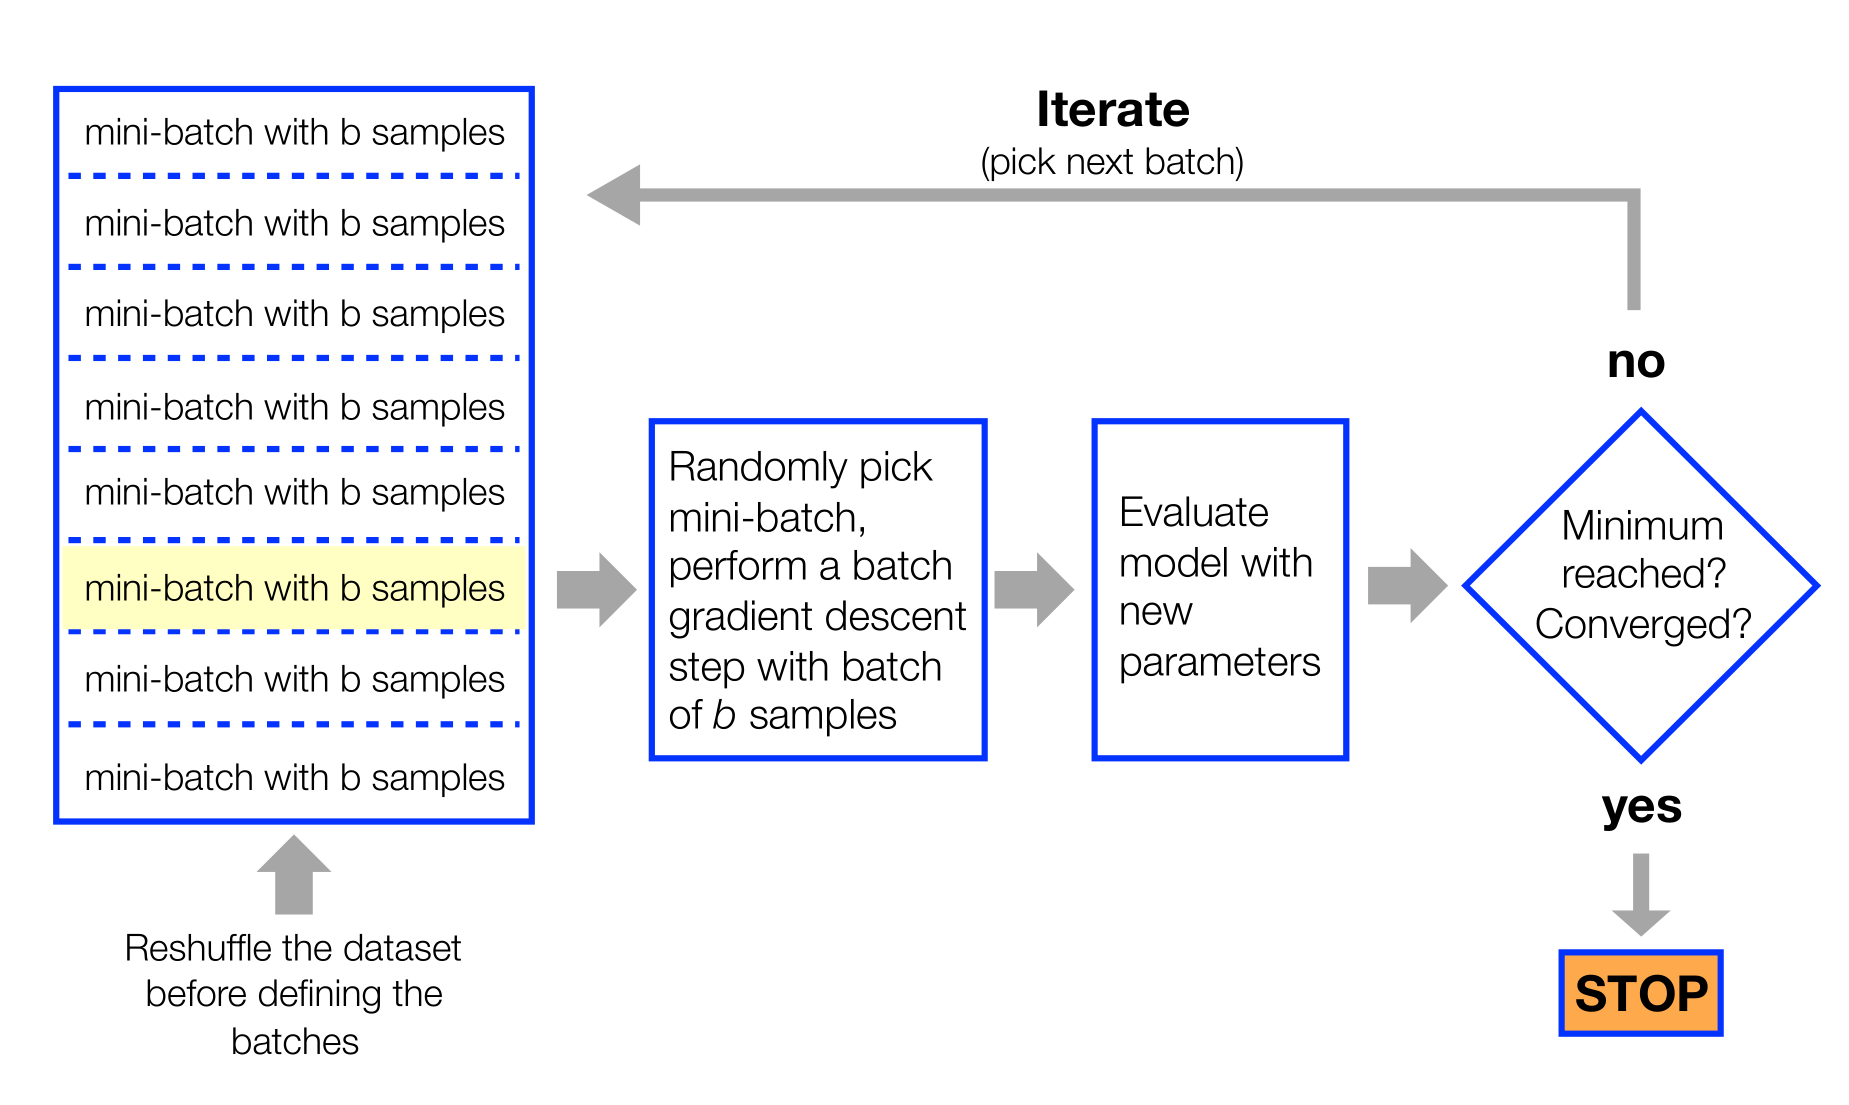
\includegraphics[width=0.7\linewidth, keepaspectratio]{img/mini_batch_gradient_descent_flow}
	\caption{Flow diagram of Mini-Batch Gradient Descent}
	\label{fig:minibatchgradientdescentflow}
\end{figure}

\subsubsection{Mini-Batch Gradient Descent for Simple Binary Classification with Cross Entropy Loss}

\begin{enumerate}
	\item Start with some inital $\theta = (b,\textbf{w})$
	\item Select mini-batch of $b$ training samples with indices $i_1, ..., i_b$ at random\\
	\begin{equation*}
		 (\textbf{x}^{(i_1)}, y^{(i_1)}), ..., (\textbf{x}^{(i_b)}, y^{(i_b)})
	\end{equation*}
	and perform the update of the $\theta$ with this sample\\
	\begin{align*}
	\textbf{w} &\leftarrow \textbf{w} - \alpha \sum_{j=1}^{b} \left(h_\theta(\textbf{x}^{(i_j)}) - y^{(i_j)}\right) \textbf{x}^{(i_j)}\\
	b &\leftarrow b - \alpha \sum_{j=1}^{b} \left(h_\theta(\textbf{x}^{(i_j)}) - y^{(i_j)}\right)
	\end{align*}
	\item Loop step 2. until convergence
\end{enumerate}

\begin{figure}[tbh]
	\centering
	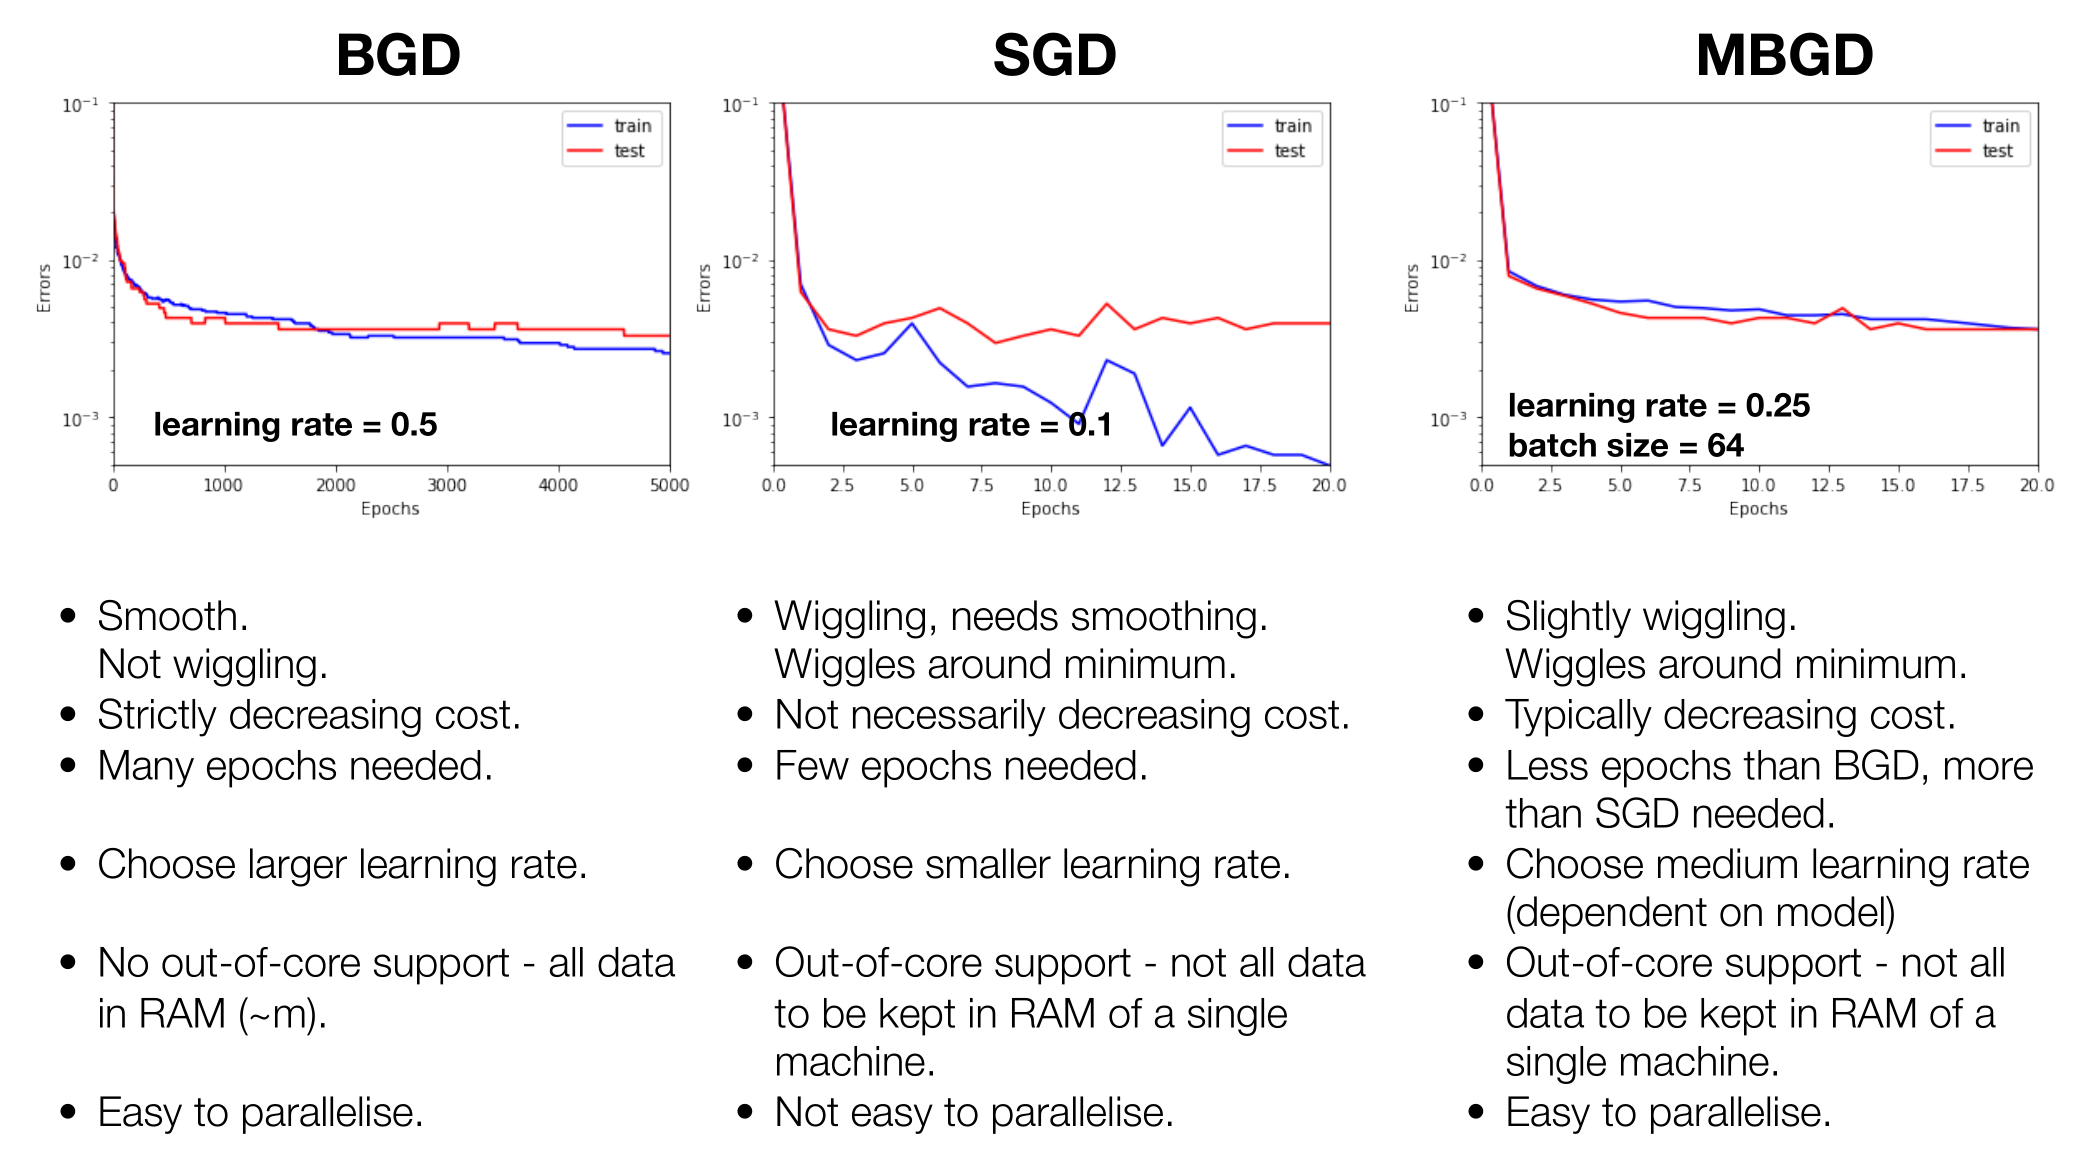
\includegraphics[width=0.8\linewidth, keepaspectratio]{img/comparison_gradient_descent}
	\caption{Comparison between the different Gradient Descent methods}
	\label{fig:comparisongradientdescent}
\end{figure}

\section{Multi-Class Classification and Softmax}

\subsection{Multiple Binary Classifiers for Multi-Class Classification}

\begin{minipage}{0.7\linewidth}
	\begin{itemize}[label=, leftmargin=*]
		\item Class labels ($K$ classes): $0\leq l < K$
		\item Structured as $K$ independent binary classification problems:\\
		$$ h_{\theta_l}(\textbf{x}) = \sigma(\textbf{w}_l\cdot\textbf{x} + b_l) $$
		$\theta_l = (\textbf{w}_l, b_l)$\quad Model parameters for class $l$, where each class is trained individually
		\item Predicted class $ \widehat{y}(\textbf{x}) = \underset{l}{\text{argmax}}\{h_{\theta_l}(\textbf{x})\} \in \{0,1,...,K-1\}$
	\end{itemize}
	
	However, as each class is trained separately and independent from the rest, the model is not trained to provide normed probabilities over all the classes. This means that the system is not forced to decide between one of the classes during training.
\end{minipage}
\begin{minipage}{0.3\linewidth}
	\centering
	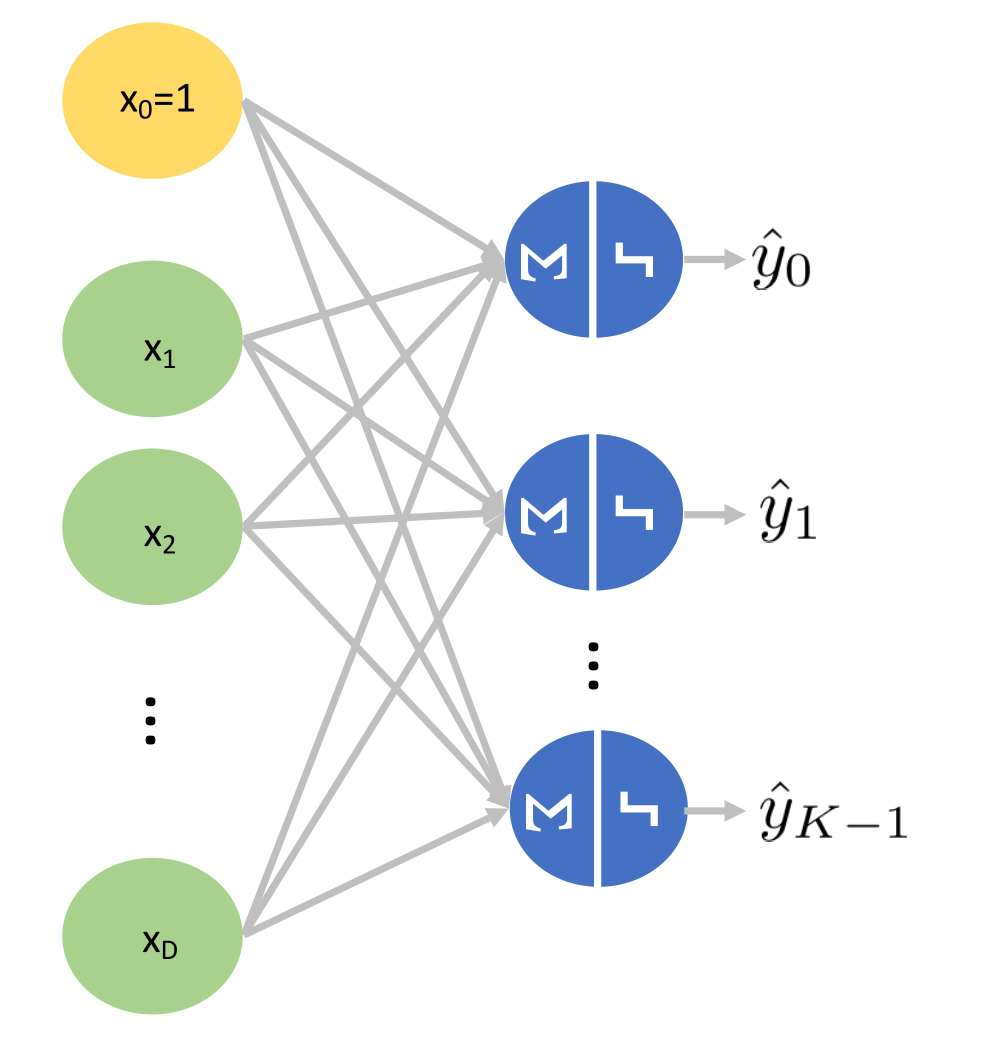
\includegraphics[width=\linewidth]{multiple_binary_classes}
\end{minipage}

\subsection{Multi-Classification with Softmax}
\paragraph{softmax function}
\begin{equation*}
	p_l = \text{softmax}(\textbf{z})_l = \frac{\exp(\textbf{z}_l)}{\sum_{j=0}^{K}\exp(\textbf{z}_j)}
\end{equation*}

where $z_l = \textbf{w}_l\cdot\textbf{x} + b_l, 0\leq l < K$ or as a vector $ \textbf{z} = \textbf{W}\cdot\textbf{x} + \textbf{b}$

\paragraph{Properties}
\begin{itemize}
	\item Normed: $\sum_{l=0}^{K-1} p_l = 1$, so the result can be interpreted as normed probabilities
	\item Peaks at the largest $z_l$. The components of softmax smoothly approximate the index of the largest element\\
	$$ p_l \approx \delta_{l, \text{argmax}\{z_k\}}\text{ if } z_l \gg z_k(\forall k\neq l)$$
	\item Parameters: $ \theta = \left( (\textbf{w}_1,b_1), ..., (\textbf{w}_{K-1},b_{K-1}) \right) = (\textbf{W},\textbf{b}) $
\end{itemize}

\subsubsection{Cost Function with Softmax}
The predicted class stays the same $ \widehat{y}(\textbf{x}) = \underset{l}{\text{argmax}}\{h_{\theta_l}(\textbf{x})\} \in \{0,1,...,K-1\}$, but $h_{\theta, l}(\textbf{x})$ is now a probability distribution for the different classes.
\begin{equation*}
	p(y=l|\textbf{x},\theta) = h_{\theta, y}(\textbf{x})
\end{equation*}

The cost function is the cross entropy in accordance with the maximum likelihood principle
\begin{align*}
	J_{CE}(\theta) &= -\frac{1}{m}\sum_{i=1}^{m}\log\left( p(y^{(i)}|\textbf{x}^{(i)}, \theta) \right)\\
	&= -\frac{1}{m}\sum_{i=1}^{m}\log\left( h_{\theta, y^{(i)}}(\textbf{x}^{(i)}) \right)
\end{align*}

\noindent
\begin{minipage}{0.5\linewidth}
	The mapping provided by the softmax function is a specific form of neuron with $m$ inputs and $m$ outputs. The inputs $\textbf{z} = (z_1,...,z_m)$ are computed by an affine transformation from the D dimension input $\textbf{x}$ (with weights matrix $\textbf{W}$ and bias vector $\textbf{b}$).
	
	The outputs $p_1, ..., p_K$ can be interpreted as normed probabilities associated with the different classes. Theses ingredients form a \emph{softmax layer} which is typically used as a final layer in classification problems.
\end{minipage}
\begin{minipage}{0.5\linewidth}
	\centering
	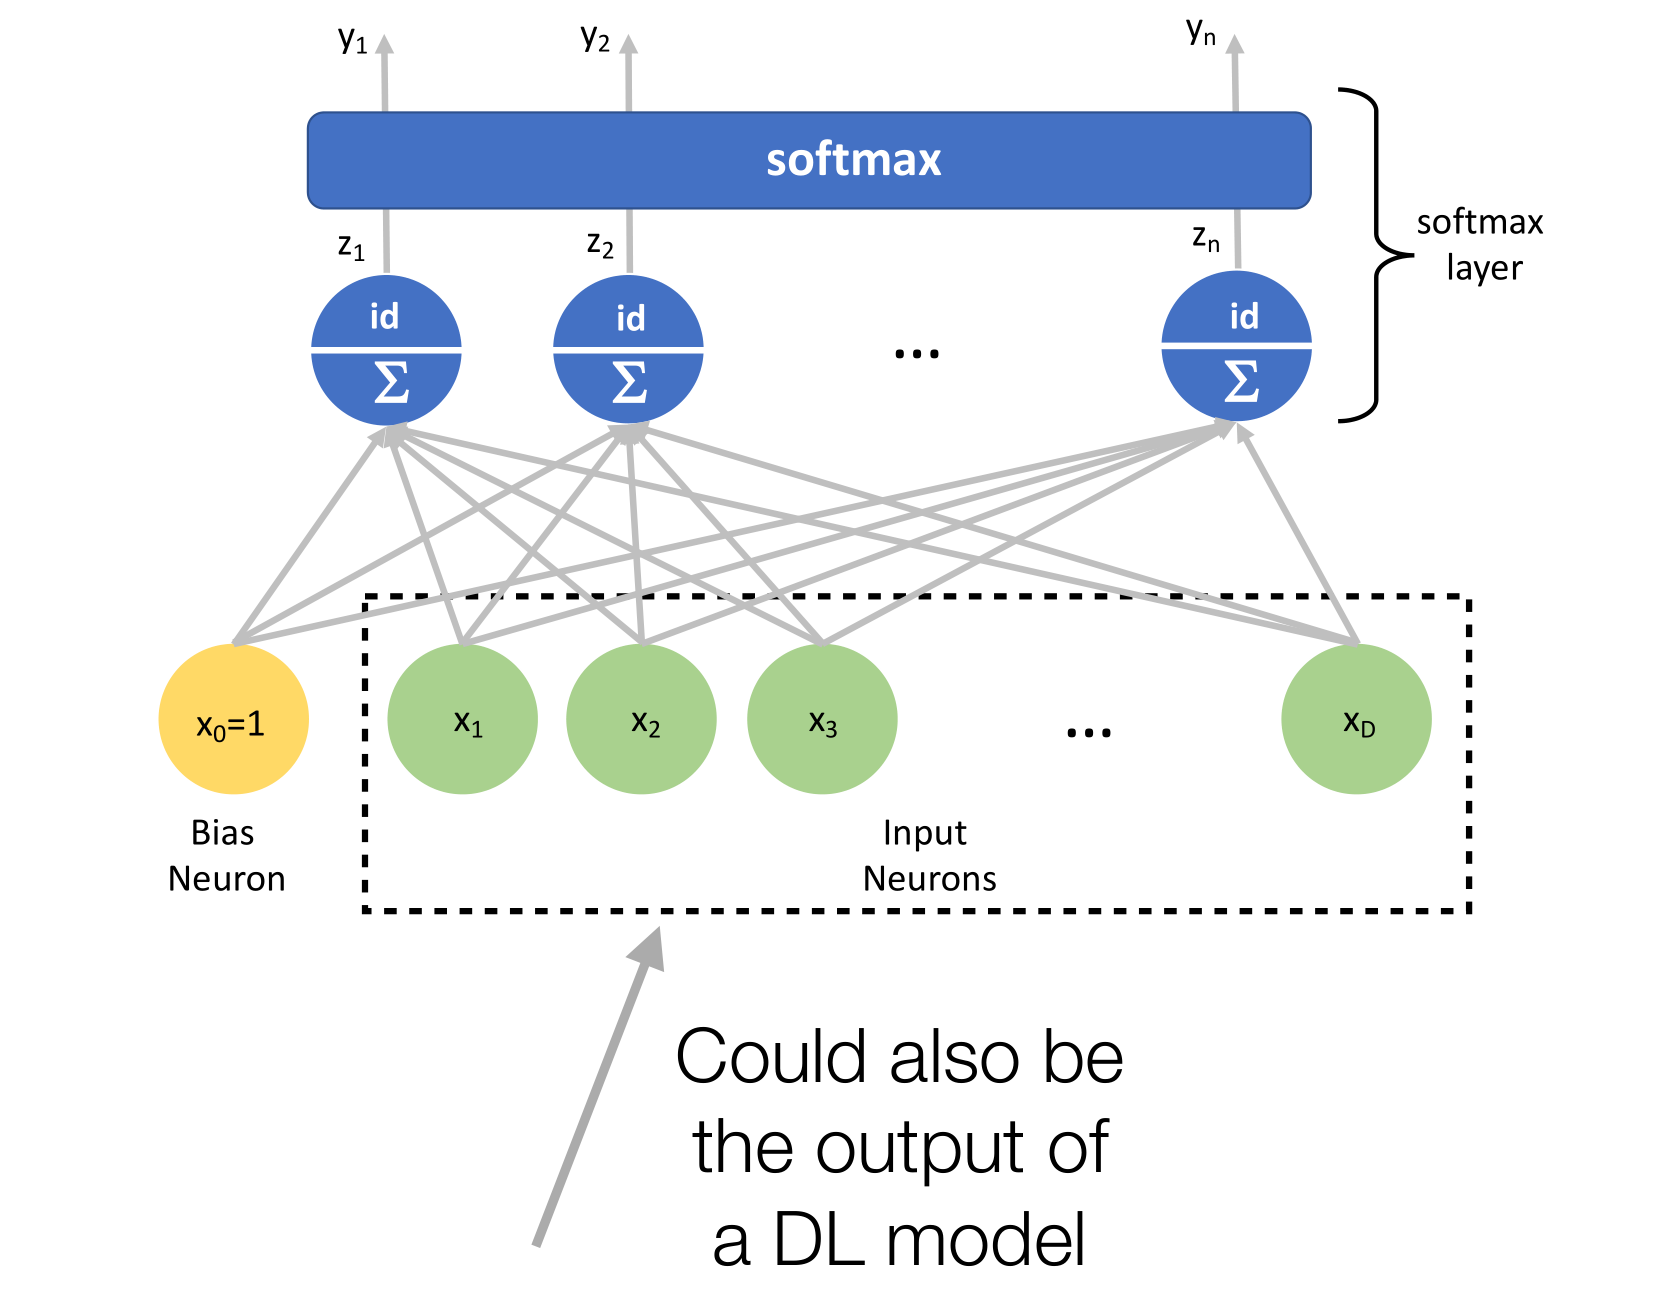
\includegraphics[width=\linewidth]{softmax_layer}
\end{minipage}

\subsubsection{Calculation of the Gradient}

With the output of the softmax layer $h_{\theta, l}(\textbf{x}$ differentiated in respect to the true label $z_k$

\begin{equation*}
	\frac{\partial h_{\theta, l}(\textbf{x})}{\partial z_k} = \delta_{l,k}h_{\delta,l}(\textbf{x}) - h_{\delta, l}(\textbf{x})h_{\delta, k}(\textbf{x})
\end{equation*}

\noindent
one obtains the gradient in respect to the weights
\begin{align*}
	\frac{\partial}{\partial \textbf{w}_j} J_{\text{CE}}(\theta) &= -\frac{1}{m} \sum_{i=1}^{m}\frac{\partial}{\partial \textbf{w}_j}\log\left(h_{\theta, y^{(i)}} (\textbf{x}^{(i)}) \right)\\
	&= -\frac{1}{m} \sum_{i=1}^{m}\frac{1}{h_{\theta, y^{(i)}} (\textbf{x}^{(i)})}\frac{\partial h_{\theta, y^{(i)}} (\textbf{x}^{(i)})}{\partial\textbf{w}_j}\\
	&= -\frac{1}{m} \sum_{i=1}^{m}\frac{1}{h_{\theta, y^{(i)}} (\textbf{x}^{(i)})}\frac{\partial h_{\theta, y^{(i)}} (\textbf{x}^{(i)})}{\partial z_j}\frac{\partial z_j}{\partial\textbf{w}_j}\\
	&= -\frac{1}{m} \sum_{i=1}^{m}\frac{1}{h_{\theta, y^{(i)}}} \left( \delta_{j, y^{(i)}} h_{\theta, j}(\textbf{x}^{(i)}) - h_{\theta, j} (\textbf{x}^{(i)}) h_{\theta, y^{(i)}}(\textbf{x}^{(i)}) \right) \frac{\partial z_j}{\partial\textbf{w}_j}\\
	&= -\frac{1}{m} \sum_{i=1}^{m}\left( \delta_{j, y^{(i)}} - h_{\theta, y^{(i)}} (\textbf{x}^{(i)}) \right)\textbf{x}^{(i)}
\end{align*}

\noindent
with $\delta_{k,j} = \left\{ \begin{matrix}
	1 & (k=j)\\
	0 & (k\neq j)
\end{matrix} \right.$ being the \textbf{Kronecker symbol}.

\vspace{1em}
\noindent
Gradient with respect to the weights and biases of the softmax layer
\begin{align*}
	\frac{\partial}{\partial \textbf{w}_j} J_{\text{CE}}(\theta) &= -\frac{1}{m} \sum_{i=1}^{m}\left( \delta_{j, y^{(i)}} - h_{\theta, y^{(i)}} (\textbf{x}^{(i)}) \right)\textbf{x}^{(i)}\\
	\frac{\partial}{\partial b_j} J_{\text{CE}}(\theta) &= -\frac{1}{m} \sum_{i=1}^{m}\left( \delta_{j, y^{(i)}} - h_{\theta, y^{(i)}} (\textbf{x}^{(i)}) \right)
\end{align*}

\vspace{1em}
\noindent
Update rules for the weights and biases of the softmax layer
\begin{align*}
	\textbf{w}_j &\leftarrow \textbf{w}_j - \alpha\frac{\partial}{\partial\textbf{w}_j}J_{\text{CE}}(\theta)\\
	b_j &\leftarrow b_j - \alpha\frac{\partial}{\partial b_j}J_{\text{CE}}(\theta)
\end{align*}

These rules apply also to the parameters of softmax layers when used as last layer of DL models.

\section{Increasing the Capacity of Models}

\subsection{Adding One Hidden Layer}
\begin{minipage}{0.5\linewidth}
	One additional layer with $n_1$ neurons using the sigmoid as the activation function. They are fully connected to the input and output neurons and posses a bias neuron (yellow in the graphic).
\end{minipage}
\begin{minipage}{0.5\linewidth}
	\centering
	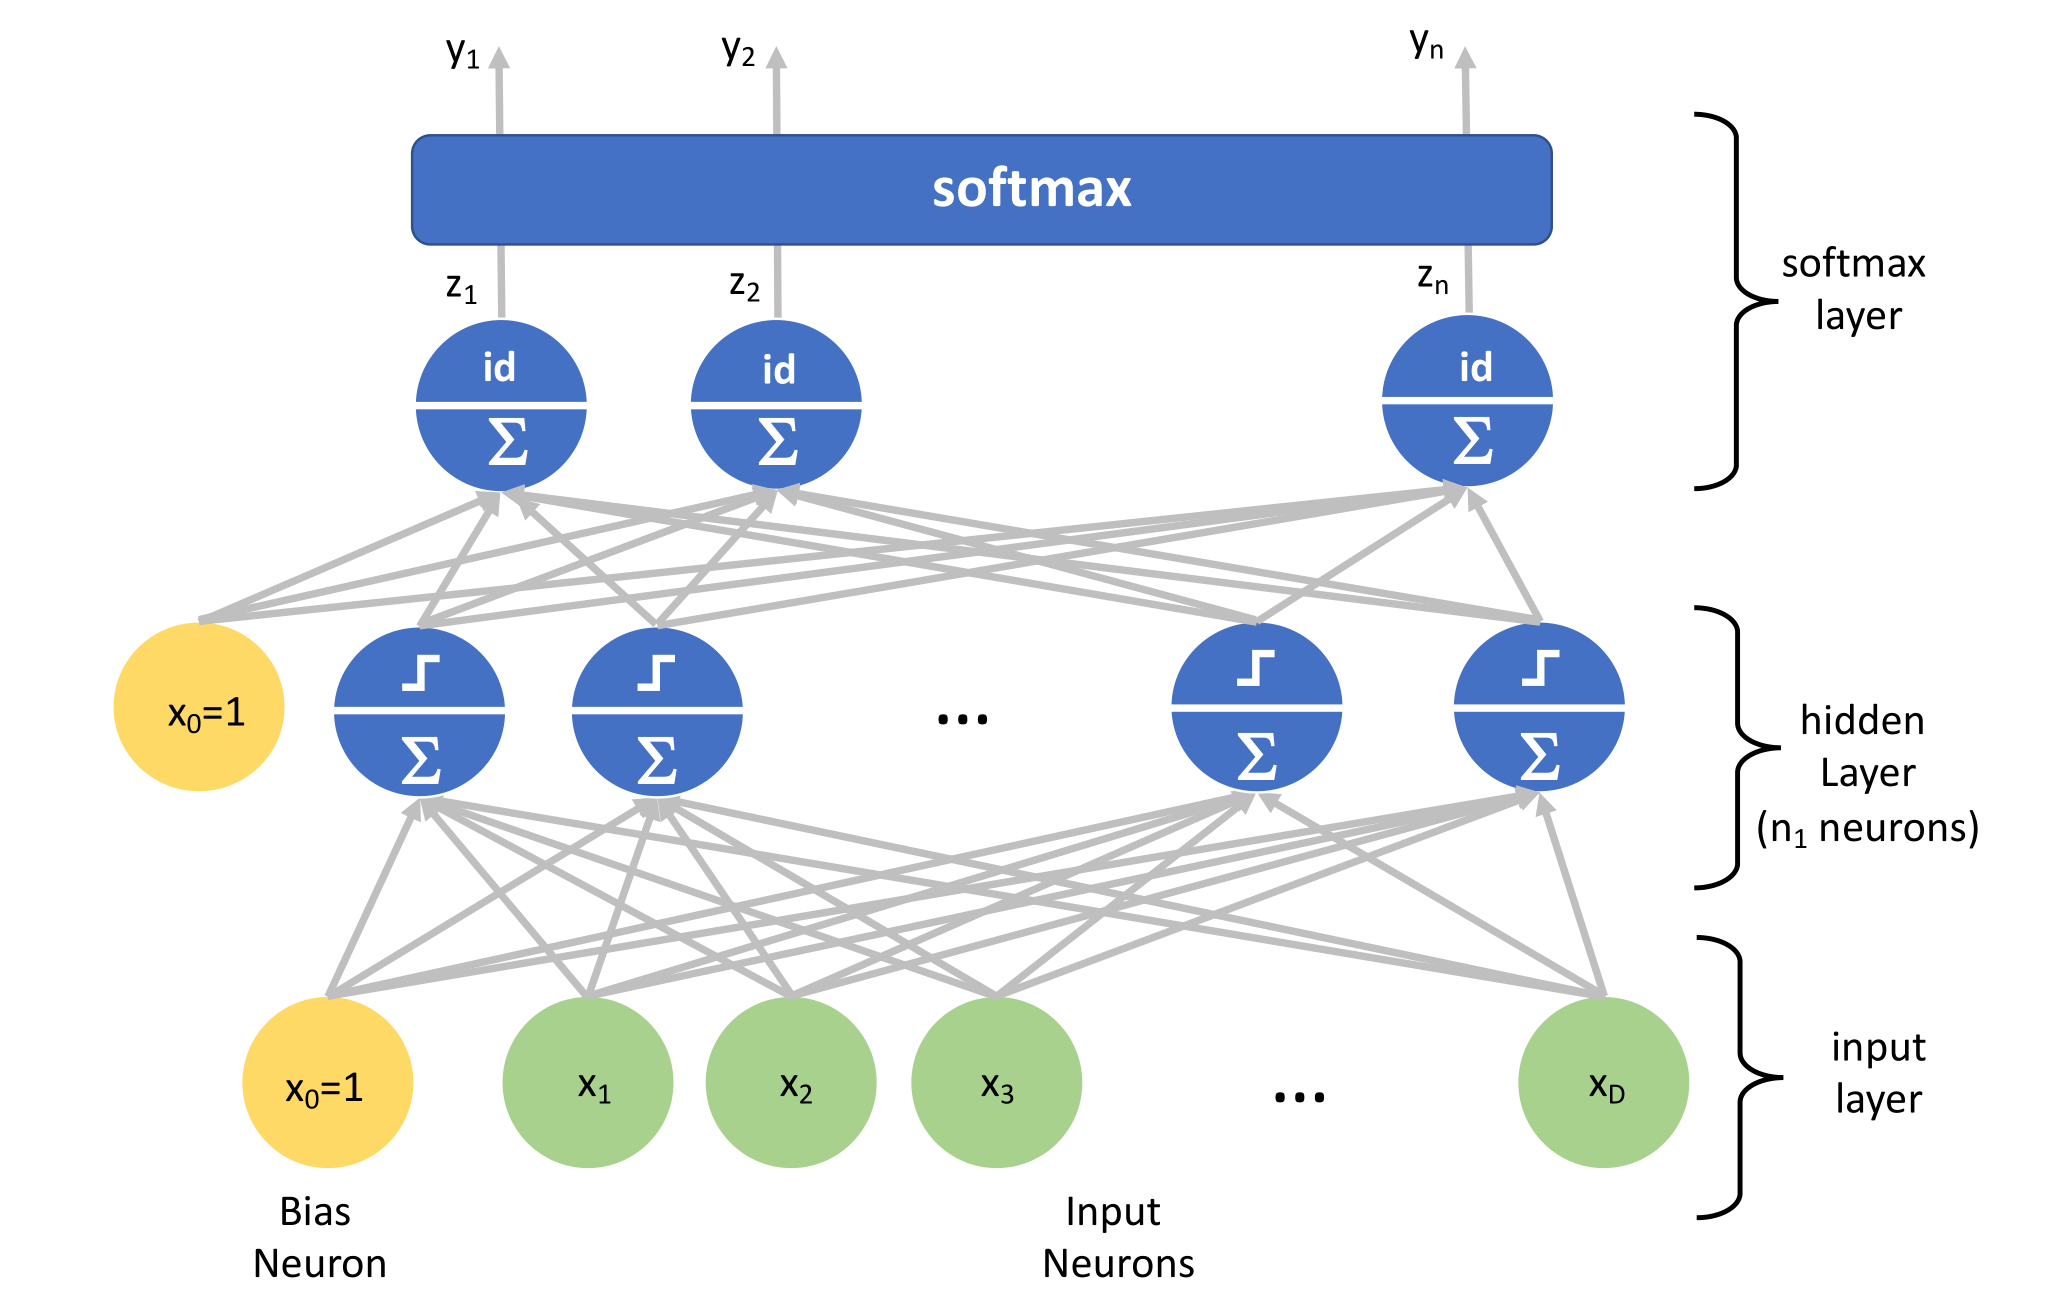
\includegraphics[width=\linewidth]{img/hidden_layer_nn}
\end{minipage}

\begin{figure}[tbh]
	\centering
	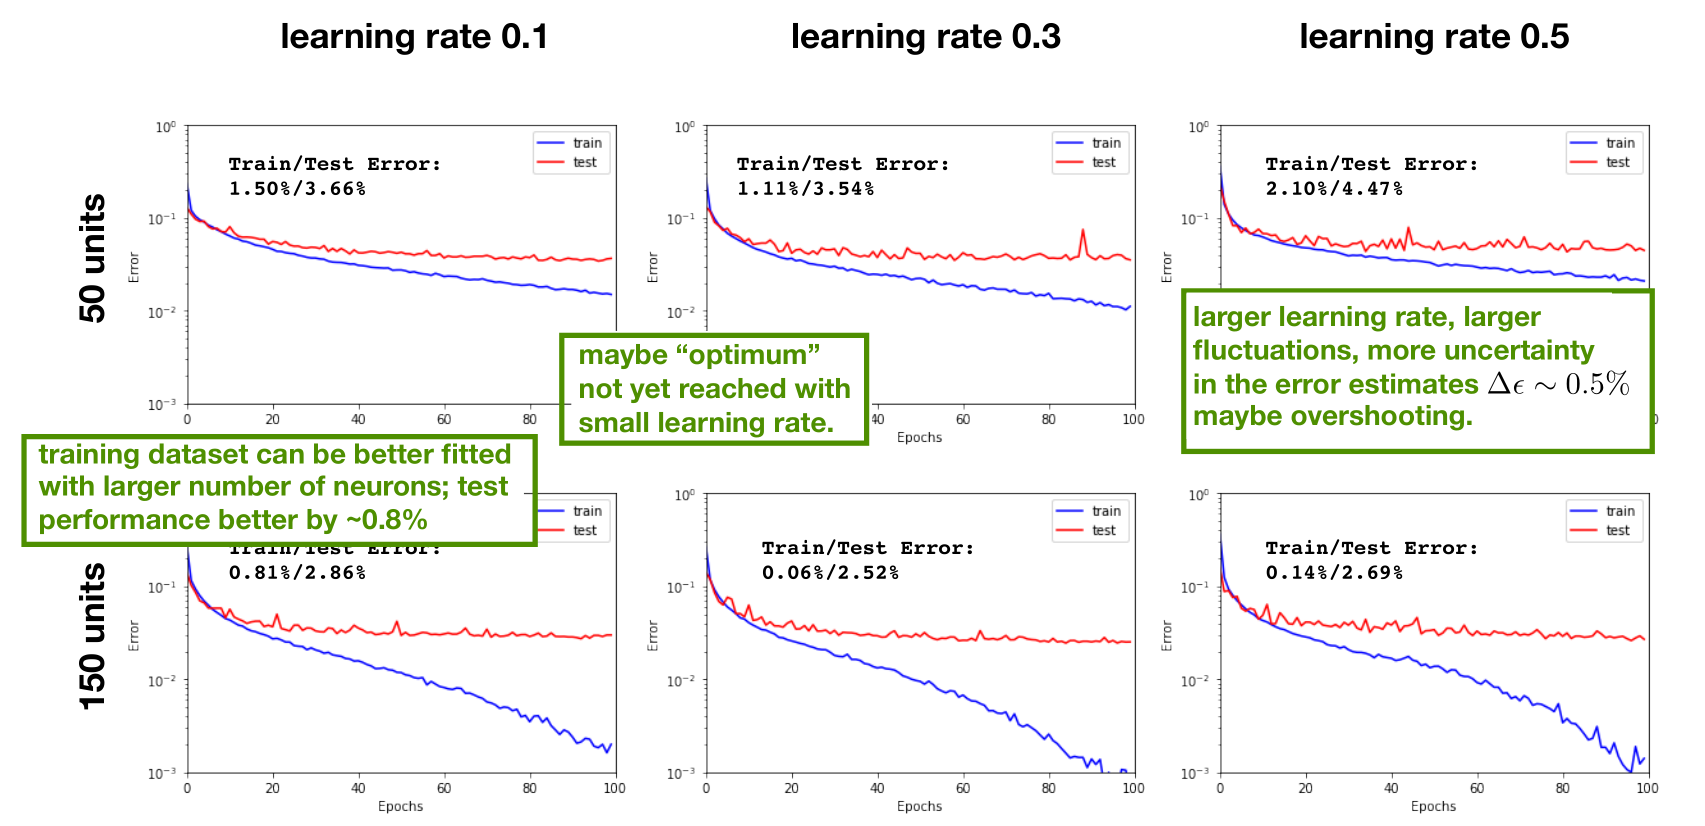
\includegraphics[width=0.8\linewidth, keepaspectratio]{img/hidden_layer_mnist_test}
	\caption{Training and Test results with a hidden layer on the MNIST set}
	\label{fig:hiddenlayermnisttest}
\end{figure}

\subsubsection{Improvements by Adding One Hidden Layer}

The error rate is reduced from ~8.0\% to ~2.4\% by only adding one hidden layer with sufficiently many neurons. By increasing the number of neurons in the hidden layer the performance improves but seems to plateau at ~200 neurons and a ~2.4\% error rate. Further improvements could be made through tuning the hyper-parameters learning rate and number of epochs, using improved optimisation schemes and Convolutional Neural Nets. Adding more hidden layers does not seem to improve the performance, one explanation could be that the correlation between pixels is already captured through one single hidden layer and that there is not much more structural information to be captured for the MNIST dataset.

\subsection{Role of the Activation Function}

Non-linearities in the mapping between input and output of a neural network are \textbf{crucial for gaining sufficient representational capacity} for learning a task with sufficient accuracy. If the activation function is linear for all neurons in a neural network, the mapping function for the neural network is linear and the representational capacity very limited. The choice of activation functions also has an impact on the robustness and performance of the learning algorithm.

\begin{tabularx}{\linewidth}{l X c}
	Function & Notes & Plot\\
	\hline
	\textbf{Heaviside}& & \\
	$f(z) = \left\{\begin{matrix}
	1 & (z \geq 0)\\
	0 & (z < 0)
	\end{matrix}\right.$ & As in Rosenblatt’s perceptron. Not differentiable. No practical use. & \imagetop{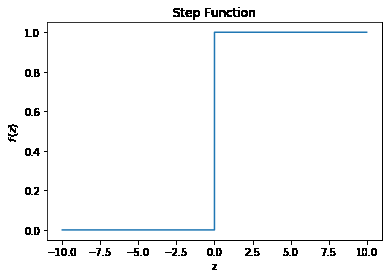
\includegraphics[width=4cm,keepaspectratio]{img/heaviside_function}}\\
	\hline
	\textbf{Sigmoid} & &\\
	$f(z)=\frac{1}{1+e^{-z}}=\frac{e^{z}}{e^{z} + 1}$ & Most commonly used in textbooks and in illustrative examples.  In practice, typically used in output layers in binary classification. Smooth and differentiable. But saturation regions leading to vanishing gradients.& \imagetop{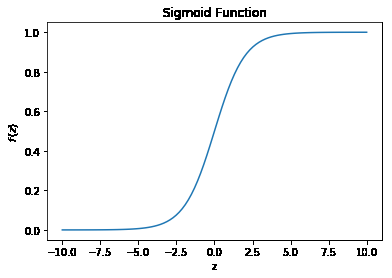
\includegraphics[width=4cm,keepaspectratio]{img/sigmoid_function}}\\
		\hline
	\textbf{Tanh} & &\\
	$f(z)=\frac{e^{z} - e^{-z}}{e^{z} + e^{-z}}$ & Often preferred over sigmoid since the output is centred around 0. Used in practice in LSTMs. Smooth and differentiable. Saturation regions leading to vanishing gradients.& \imagetop{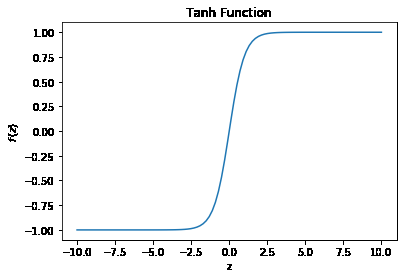
\includegraphics[width=4cm,keepaspectratio]{img/tanh_function}}\\
	\hline
	\textbf{Recti-Linear Unit} & &\\
	$f(z)=\max(0,z)$ & Used as de facto standard. Introduced to alleviate the vanishing gradient problem. Suffers from dying units problem for $z<0$ where the activation and resulting gradient is 0.& \imagetop{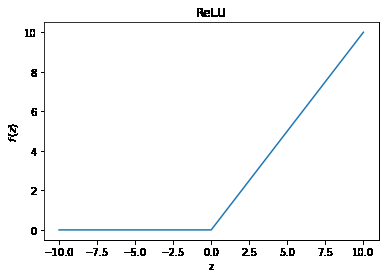
\includegraphics[width=4cm,keepaspectratio]{img/rectilinear_unit}}\\
	\hline
	\textbf{Leaky Recti-Linear Unit} & &\\
	$f(z)=\max(\alpha\cdot z,z)$ & Alleviates both, the vanishing gradient problem and the dying units problem. Uses a small hyperparameter $0<\alpha<1$ which ensures that the unit never dies (typical default $\alpha = 0.01$).& \imagetop{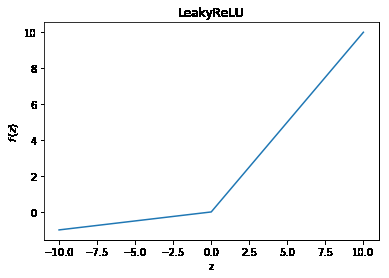
\includegraphics[width=4cm,keepaspectratio]{img/leaky_rectilinear_unit}}\\
	\hline
	\textbf{Exponential Linear Unit}& & \\
	$f(z) = \left\{\begin{matrix}
	\alpha(e^{z} - 1) & (z < 0)\\
	z & (z \geq 0)
	\end{matrix}\right.$ & Similar to Leaky ReLU. Negative activation stabilises at $-\alpha$. Gradient vanishes at small negative values. More expensive to compute.& \imagetop{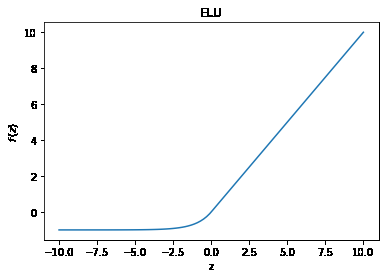
\includegraphics[width=4cm,keepaspectratio]{img/exponential_linear_unit}}\\
	\hline
	\pagebreak
	& & \\
	\hline
	\textbf{Identity} & &\\
	$f(z)=z$ & Used only in specific cases such as in the last layer of a network for performing a regression task.& \imagetop{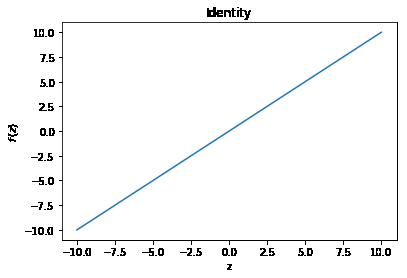
\includegraphics[width=4cm,keepaspectratio]{img/identity_function}}\\
	\hline
	\textbf{Softmax} & &\\
	$f(\textbf{z})_l= \frac{e^{z_l}}{\sum_{j=1}^{l}e^{z_j}}$ & Used as last layer in a network for a classification task with $l$ classes. Output vector can be interpreted as probability distribution.& \imagetop{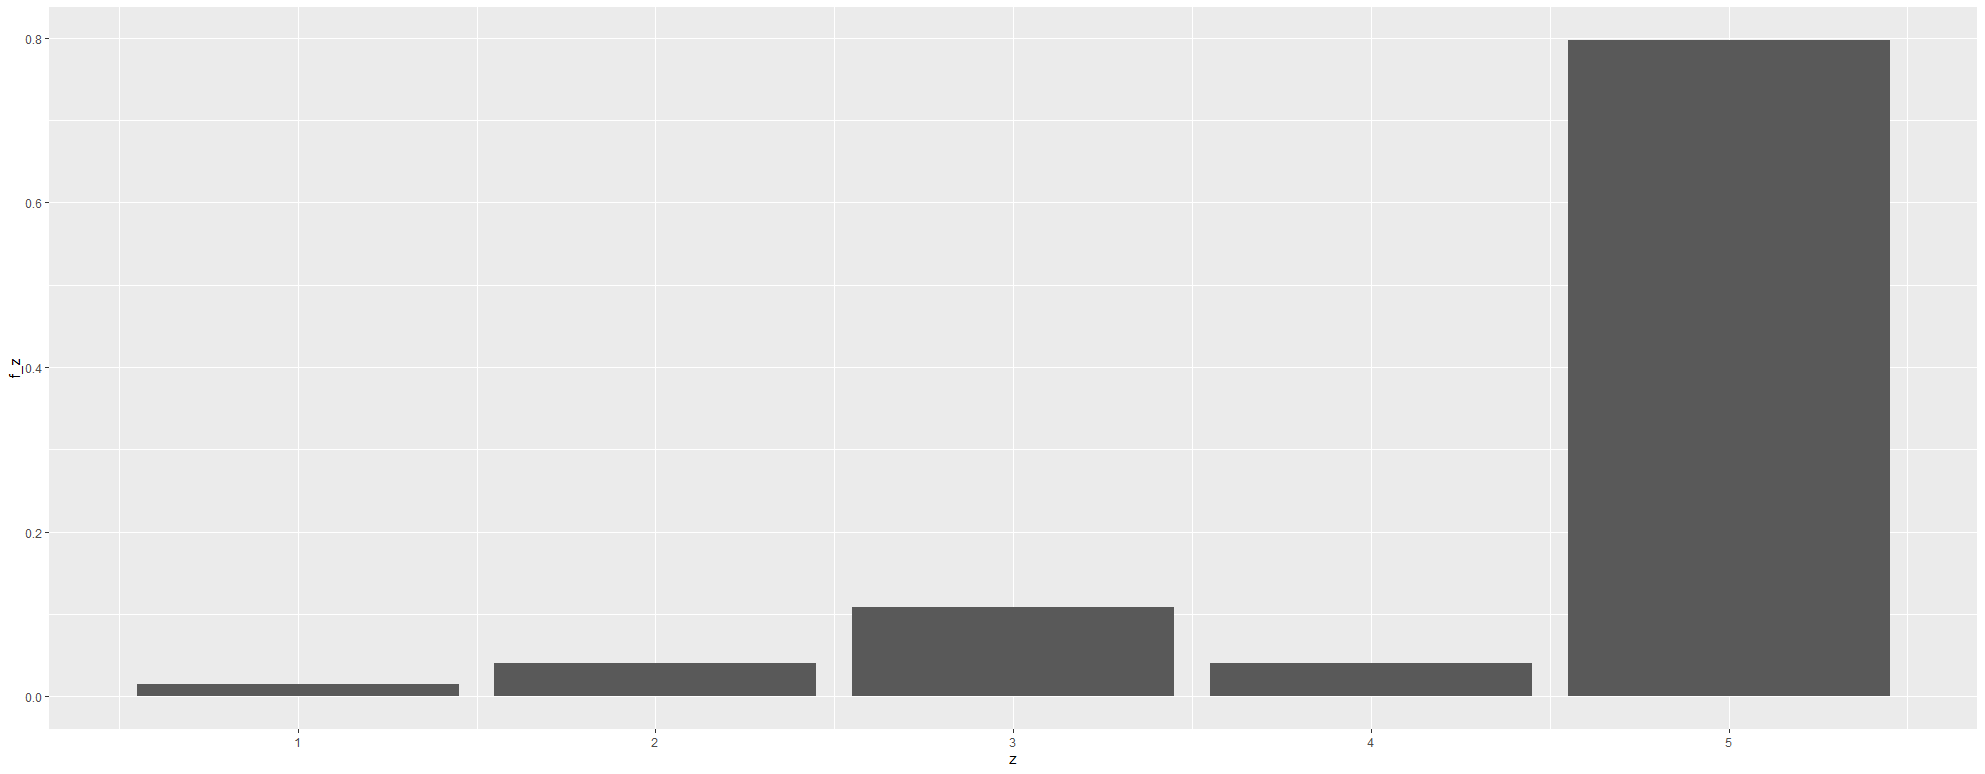
\includegraphics[width=4cm,keepaspectratio]{img/softmax_function}}\\
	\hline
\end{tabularx}

\section{Universal Function Approximation}
Neural networks provide models for predicting an outcome $y$ from an input $\textbf{x}$. In general, we expect to find only an approximate mapping $\textbf{x}\rightarrow y$. The mapping  is approximated by searching in a suitable parametric family of functions $h_\theta(\textbf{x})$ with parameters $\boldsymbol{\theta}$
\begin{equation*}
	\textbf{x} \rightarrow y = h(\textbf{x}) \approx h_\theta(\textbf{x}) = \widehat{y}
\end{equation*}
The richness of this family of functions drives the ability to represent more or less complex mappings. This ability is also referred to as \emph{representational capacity}. For neural networks, the representational capacity is determined by the number of layers, type of layers, the number of neurons per layer, type of activation function, type of neuron.

\subsection{Universal Approximation Theorem}

\begin{theorem}
	A feedforward network with a linear output layer and at least one hidden layer with a non-linear ("squashing") activation function (e.g. sigmoid) can approximate a large class of functions $\mathbb{R}^{n_x} \rightarrow \mathbb{R}^{n_y}$ with arbitrary accuracy - provided that the network is given a sufficient number of hidden units and the parameters are suitably chosen.
\end{theorem}

\noindent
\begin{minipage}{0.6\linewidth}
	One-dimensional real-valued input $x$. One hidden layer with n neurons and sigmoid activation function, weights $w_{1,k}$ and bias $b_{1,k}$, one linear output layer with weights $w_{2,k}$ and biases $b_{2,k}$. The linear output layer leads to a linear combination of sigmoids
	\begin{equation*}
		h_\theta(x) = \sum_{k=1}^{n} w_{2,k}\cdot\sigma(w_{1,k}\cdot x + b_{1,k}) + b_2
	\end{equation*}
	The theorem states that any quite general function ($\mathbb{R}^1\rightarrow\mathbb{R}^1$) can be approximated if suitable parameters and a suitable number of neuron $n$ are chosen.
\end{minipage}
\begin{minipage}{0.4\linewidth}
	\centering
	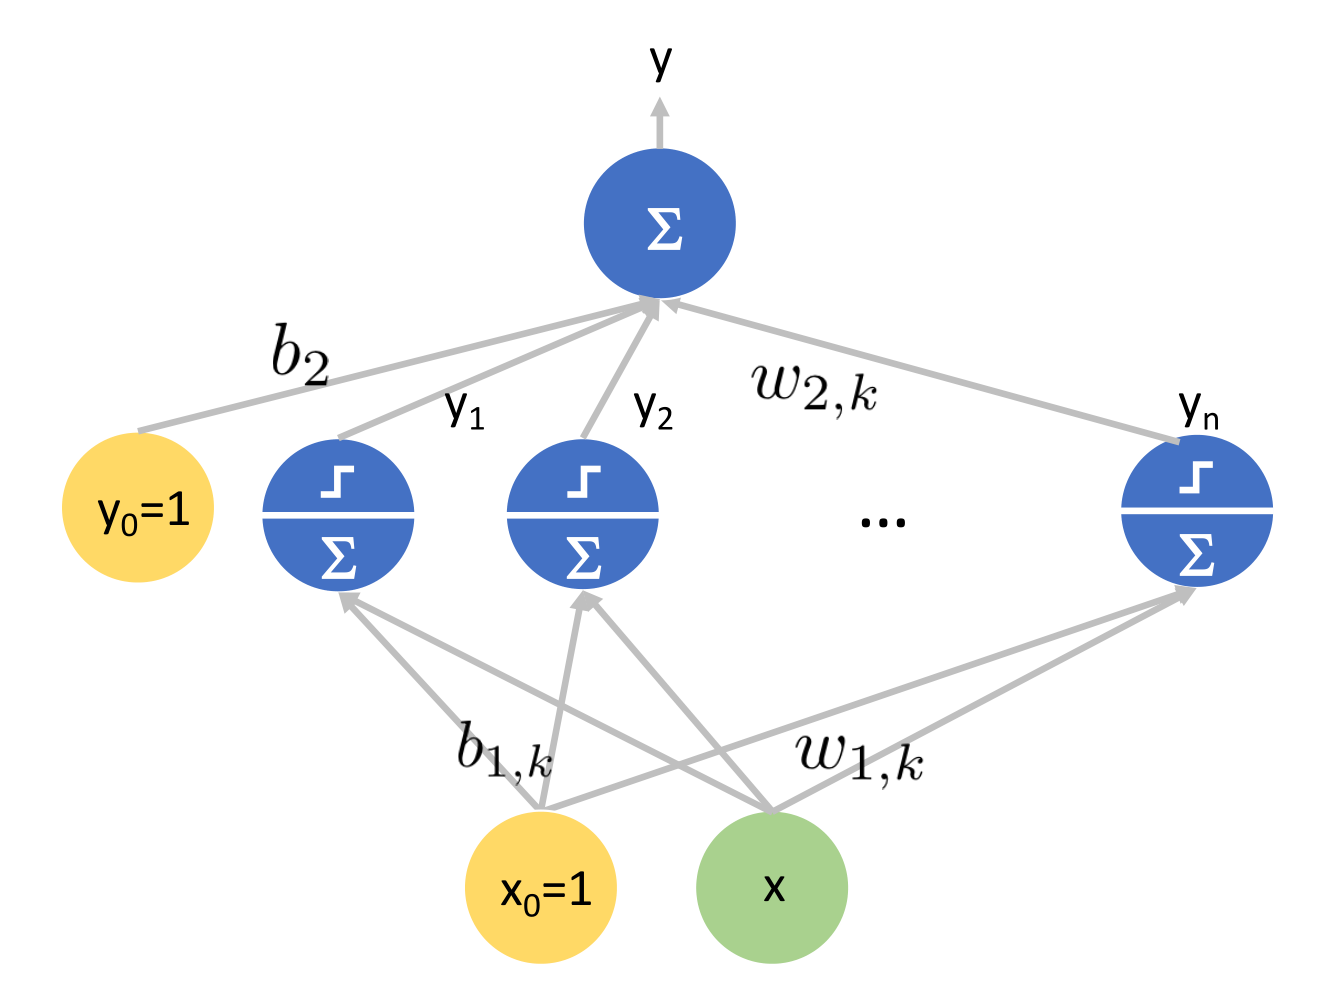
\includegraphics[width=\linewidth,keepaspectratio]{1d_function_approximation}
\end{minipage}

\vspace{1em}
\noindent
For convenience the sigmoids with the position of the ste $s = -\frac{b}{w}$ are re-parametrised so that $\sigma(w\cdot x + b) = \sigma(w\cdot(x-s))$. With the parameter $w$ the slope of the step is controlled, that is the larger $w$ the steeper the step, as indicated in the figure on the left.

\begin{figure}[H]
	\centering
	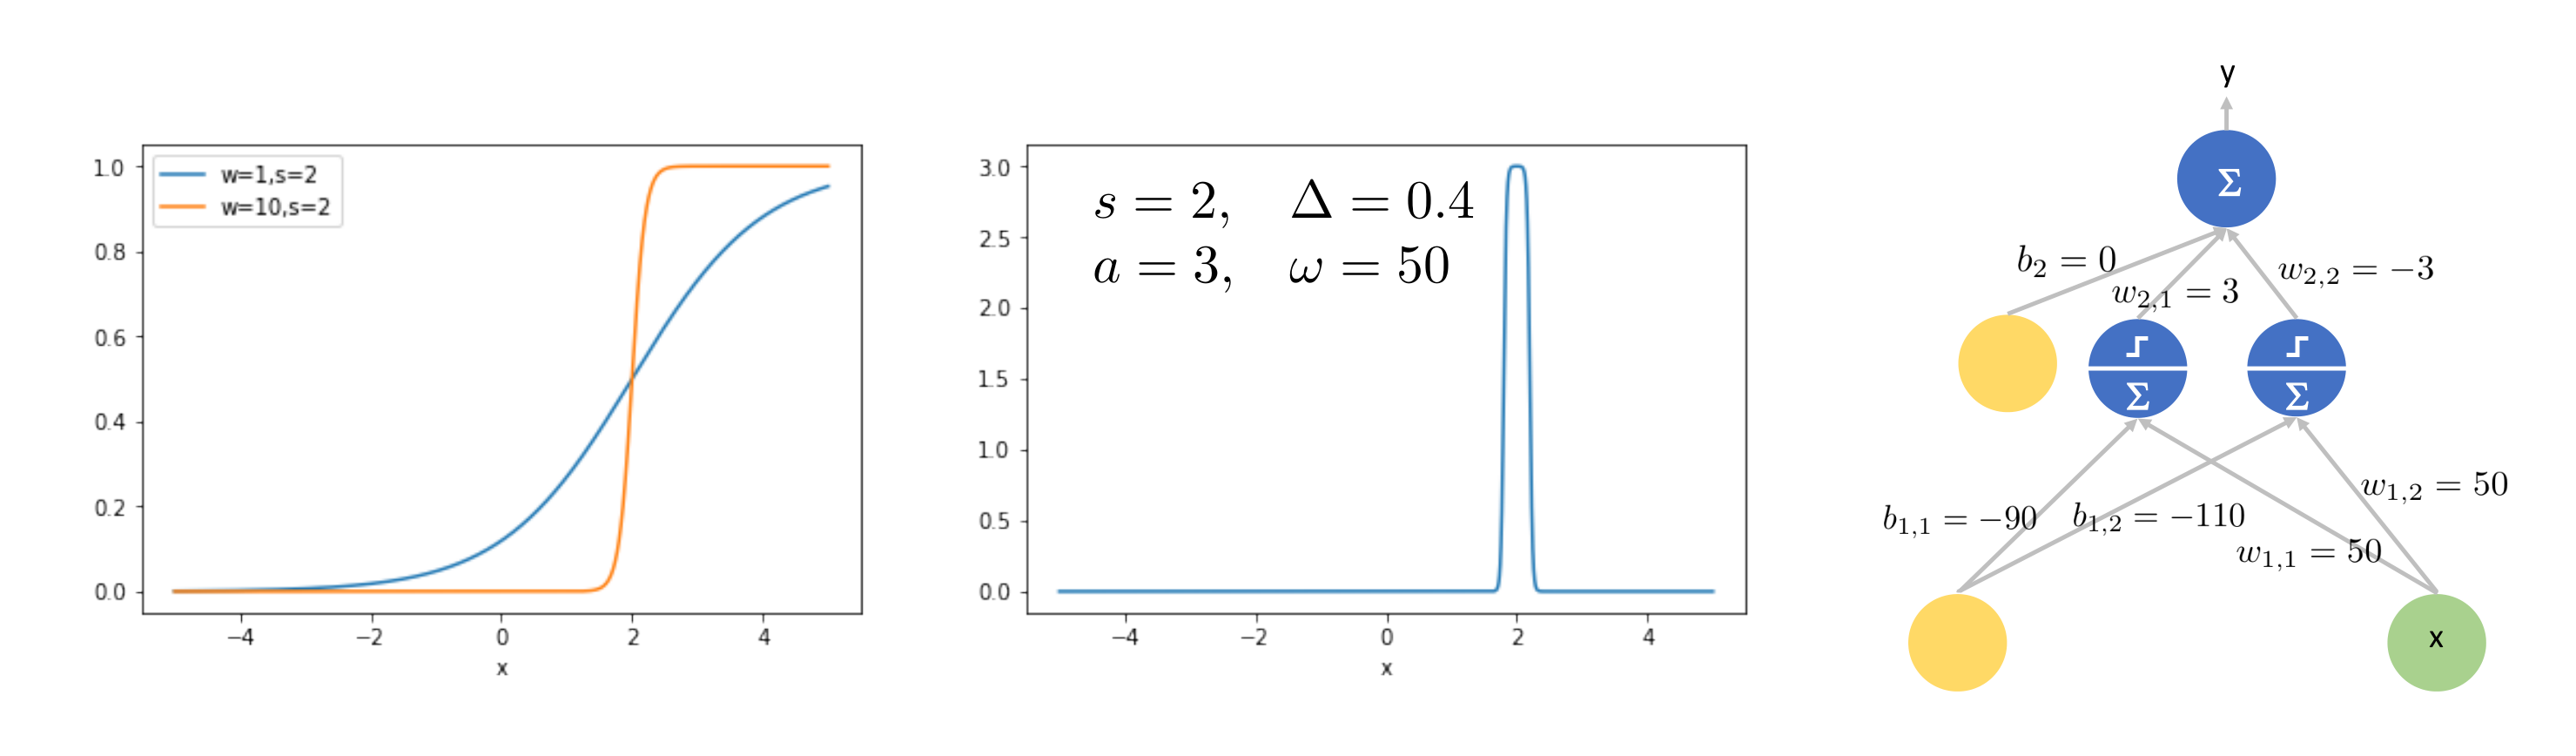
\includegraphics[width=0.8\linewidth,keepaspectratio]{1d_function_approximation_example}
\end{figure}

By combining two such step functions a peak at location s with width $\Delta$ is easily created
\begin{equation*}
	\phi(x;s,a,\Delta,w) = a\left(\sigma(w\cdot(x-s+\frac{\Delta}{2})) - \sigma(w\cdot(x-s-\frac{\Delta}{2}))\right)
\end{equation*}

\subsubsection{Generalisation to Arbitrary Functions}

The scheme for $1d$ input and $1d$ output can easily be generalised to $nd$ input and $md$ output.

\paragraph{Problems} For improving the accuracy when modelling with step-functions, more and more neurons are needed and many parameters need to be determined. In problems with high-dimensional input, an exponentially growing number of neurons is needed.

Accordingly, more data sampled on a sufficiently fine grid is needed. With growing dimensionality in the input  this becomes infeasible. This is known as curse of dimensionality.

If just the available data is used and the data between points is interpolated with step functions, the training data is significantly overfitted.

The theorem does not provide a scheme for efficiently learning the parameters from available limited data.

\section{Overfitting and Generalisation}

\subsection{Overfitting}
\begin{figure}[tbh]
	\centering
	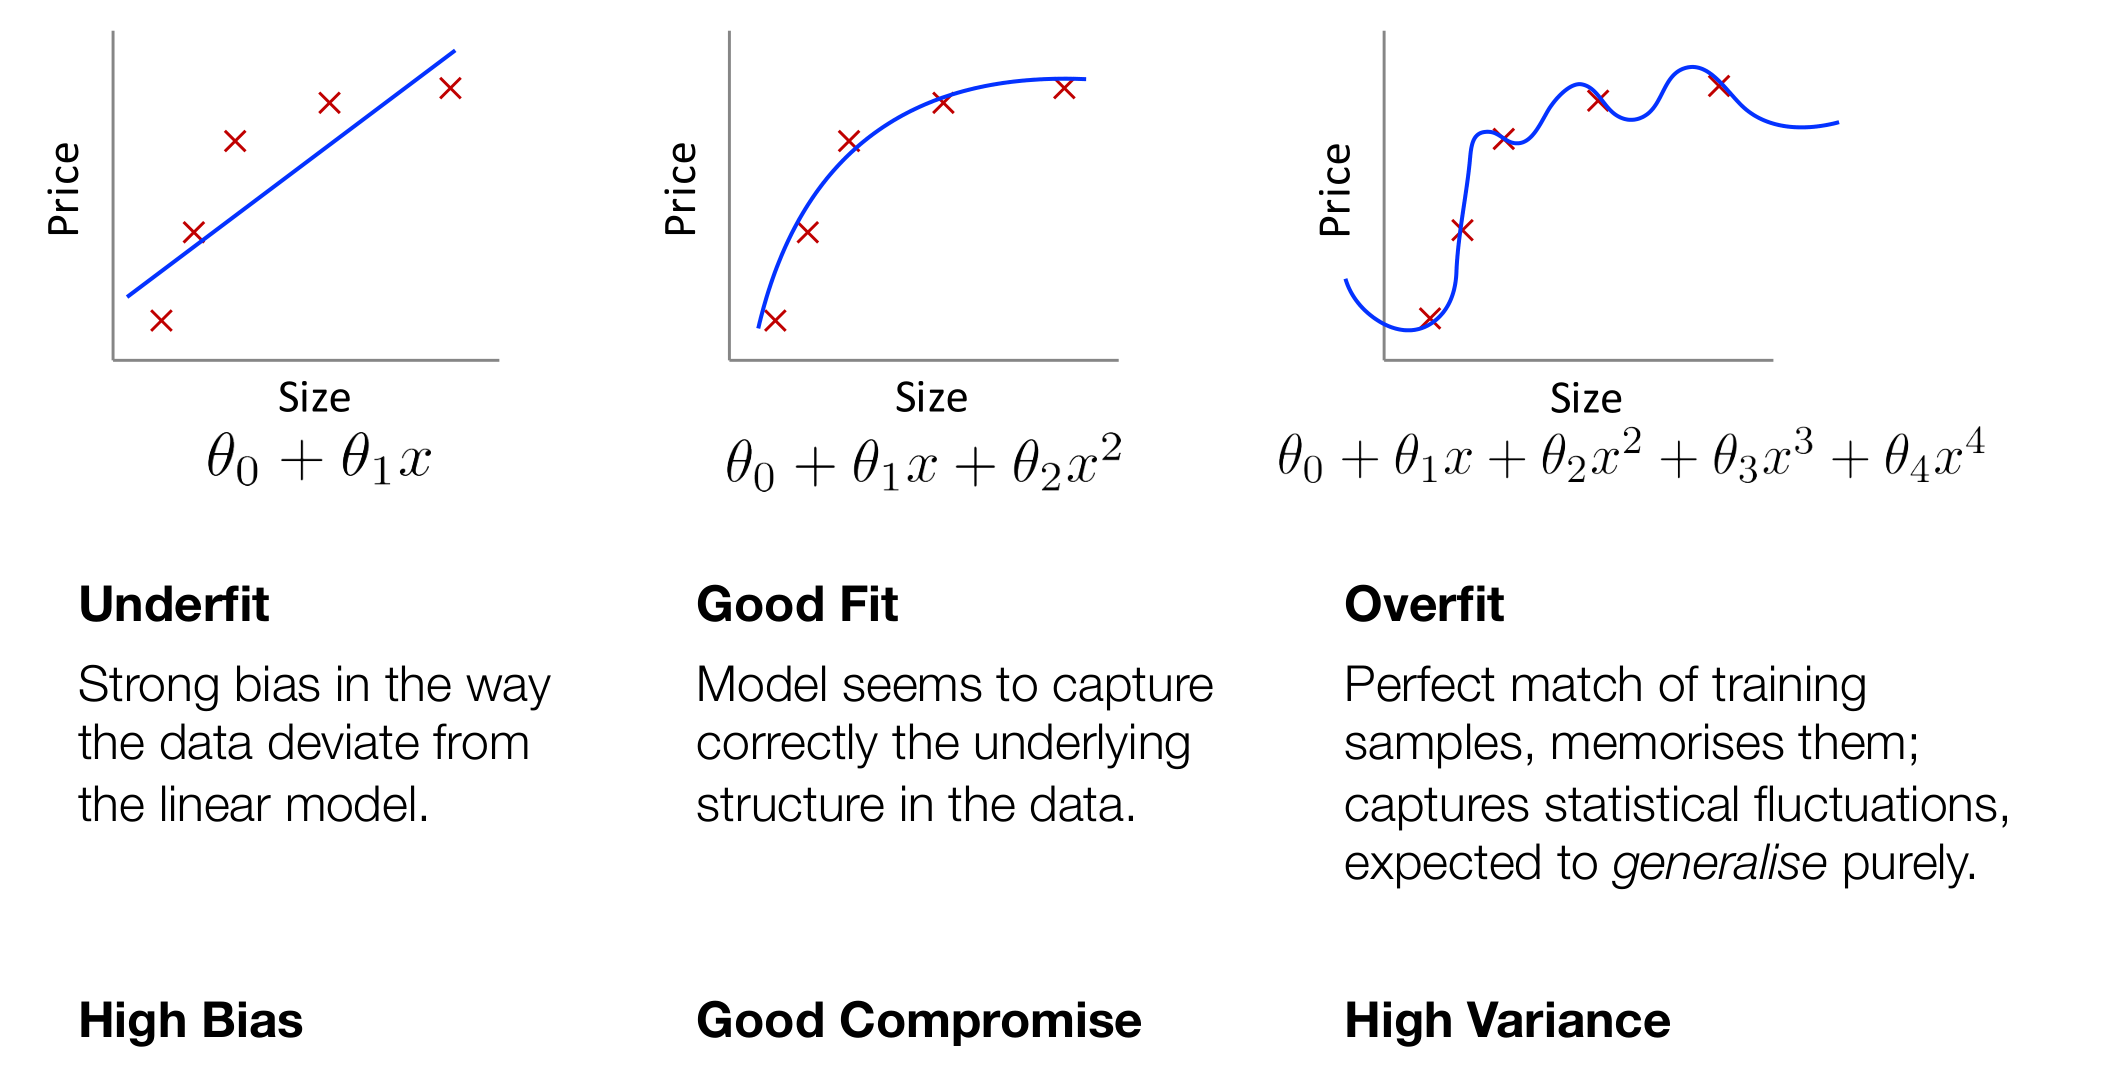
\includegraphics[width=\linewidth,keepaspectratio]{img/data_overfitting_example}
	\caption{An example of data being progressively more overfitted}
	\label{fig:dataoverfittingexample}
\end{figure}

\paragraph{Guiding Principle} Occam's Razor: Among competing hypothesis that explain known observations equally well the simplest is the best.

\subsubsection{Characterisation of Overfitting}
Overfitting occurs when the learned hypothesis (trained model) fits the training data set very well, but fails to generalise to new examples.
Overfitting can occur when
\begin{itemize}
	\item the number of parameters of the model is too large, that is the model being too flexible
	\item the training set is too small in comparison with the dimensionality of the input data, which introduces sampling noise
	\item the training set is too noisy
\end{itemize}

The problem with overfitting is, that the model is likely to detect patterns in the noise itself. These patterns are unlikely to generalise to previously unobserved new inputs. A machine learning algorithm to perform well should thus be able to make the
\begin{enumerate}
	\item training error, also called bias error, small
	\item gap between training and test error, also called variance error, small
	\item bias and variance error comparable in magnitude
\end{enumerate}

\paragraph{How to Examine Overfitting}
Evaluate the performance on the training and the test set for different models with different model complexity, by using different training set sizes and after different numbers of training epochs.

\begin{figure}[H]
	\centering
	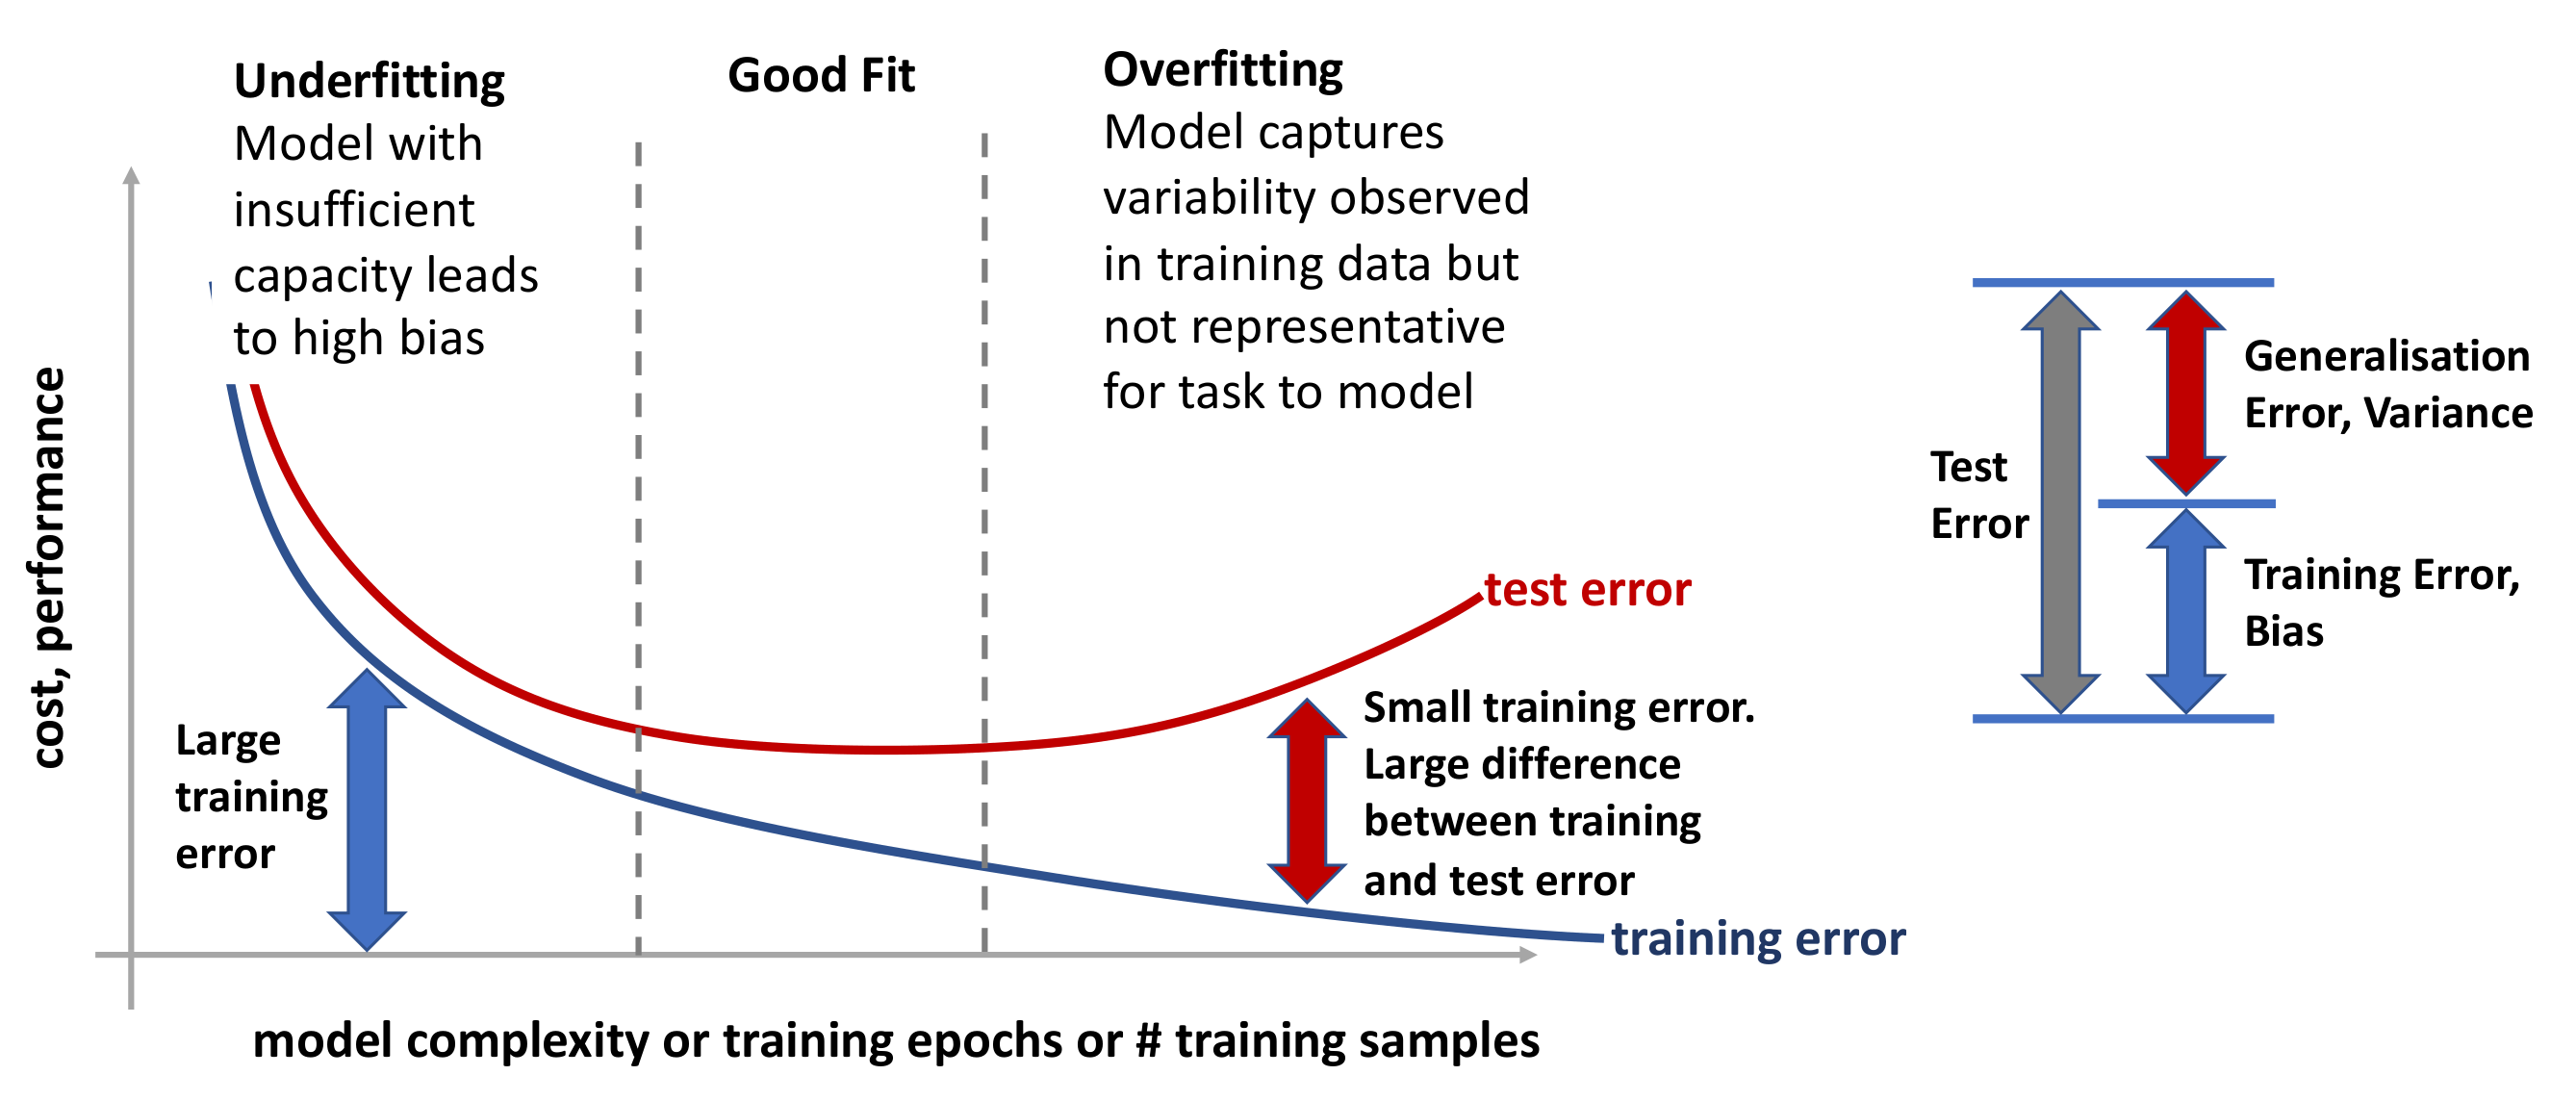
\includegraphics[width=0.9\linewidth,keepaspectratio]{test_training_set_overfitting}
	\caption{Strategies to reduce overfitting}
\end{figure}

\subsection{Model Selection}
The goal of model selection is to select the model with the best performance from a family of models. To achieve this the performance for different model with differing complexity needs to be evaluated, but to avoid overfitting on the test set, we must not use information from the test set to determine the hyper-parameters of the model.

The solution is to further split the original training set into two subsets, a training set used for training the models, and a validation set used for evaluating the performance and selection of the model and hyper-parameters.

\subsubsection{Hyper-Parameters}

Hyper-Parameters specify higher level properties of the mapping function (model) and the learning process. These parameters are not trainable (not determined by optimising the cost on the training set), but optimised on the validation set.

\vspace{1em}
\noindent
Examples of hyper-parameters are
\begin{itemize}
	\item Learning Rate
	\item Batch Size
	\item Number of hidden layers
	\item Number of neurons in a layer
	\item Number of epochs
\end{itemize}

\subsection{Training, Validation, Test Split}

\begin{tabularx}{\linewidth}{c X c || c }
	& & \multicolumn{2}{c}{typical split ratio} \\
	& & small datasets & large datasets\\
	\hline
	\textbf{Training Set} & Subset of \emph{trustable} data used to train the model & 60\% & 98\%\\
	\hline
	\textbf{Validation Set} & Subset of \emph{trustable} data used to select models, for example by selecting the best hyper-parameters of the model & 20\% & 1\%\\
	\hline
	\textbf{Test Set} & Subset of \emph{trustable} data used to measure the performance of the finally selected model & 20\% & 1\%\\
	\hline
\end{tabularx}

Trustable means in this context
\begin{itemize}
	\item composed of data acquired under the same conditions
	\item data with the same characteristics (range of value, distribution, sparseness)
	\item dataset sufficiently large to have confidence in the parameter estimates or evaluation metrics
\end{itemize}

\subsubsection{Selecting a Split Ratio}
Considering different split ratios for a given fixed dataset, it is expected that
\begin{itemize}
	\item the \textbf{training cost or training error} increases with a higher split ratio\\
		\emph{it gets more difficult to perfectly fit a model with more data}
	\item the \textbf{validation cost or validation error} decreases with a higher split ratio, the validation becomes very wiggly for large split ratios\\
		\emph{the model trained with more data is expected to capture more details about the underlying problem}
\end{itemize}

\begin{figure}[H]
	\centering
	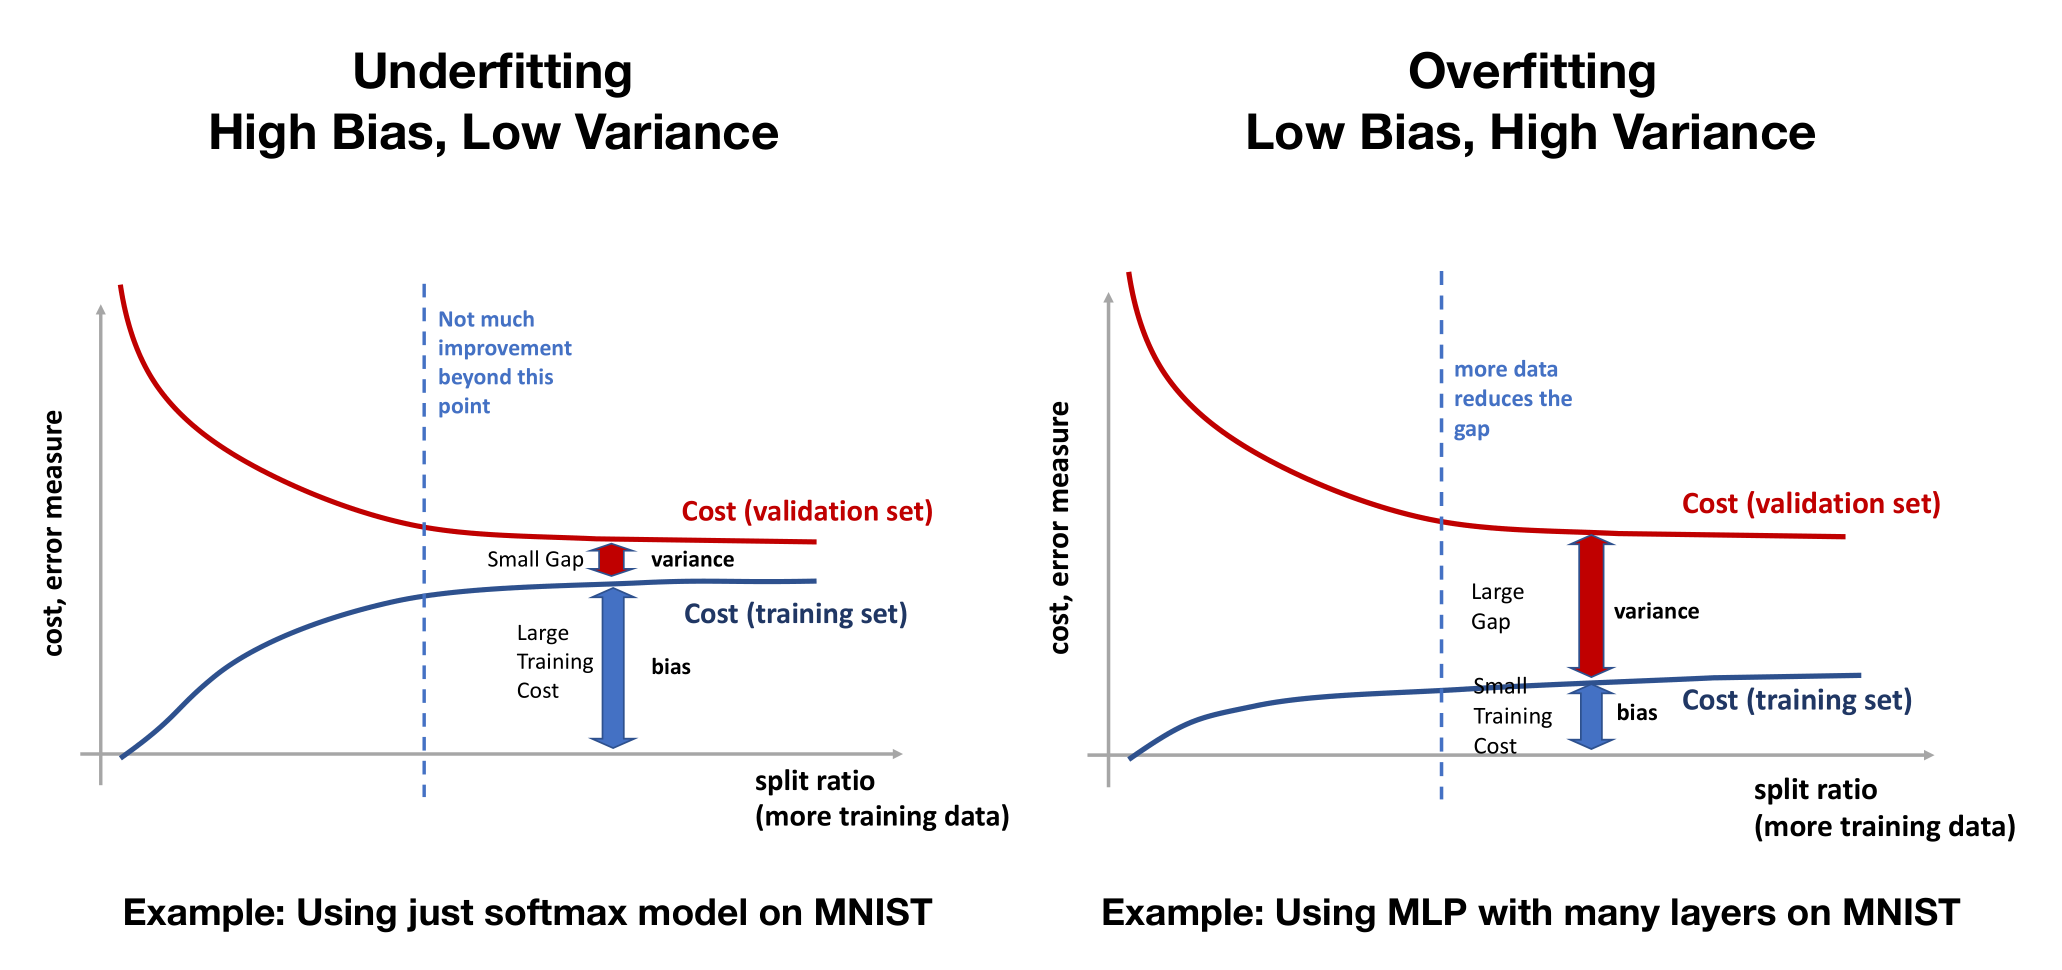
\includegraphics[width=0.9\linewidth, keepaspectratio]{learning_curve_analysis}
	\caption{Analysis of different learning curves}
	\label{fig:learningcurveanalysis}
\end{figure}

\begin{figure}[H]
	\centering
	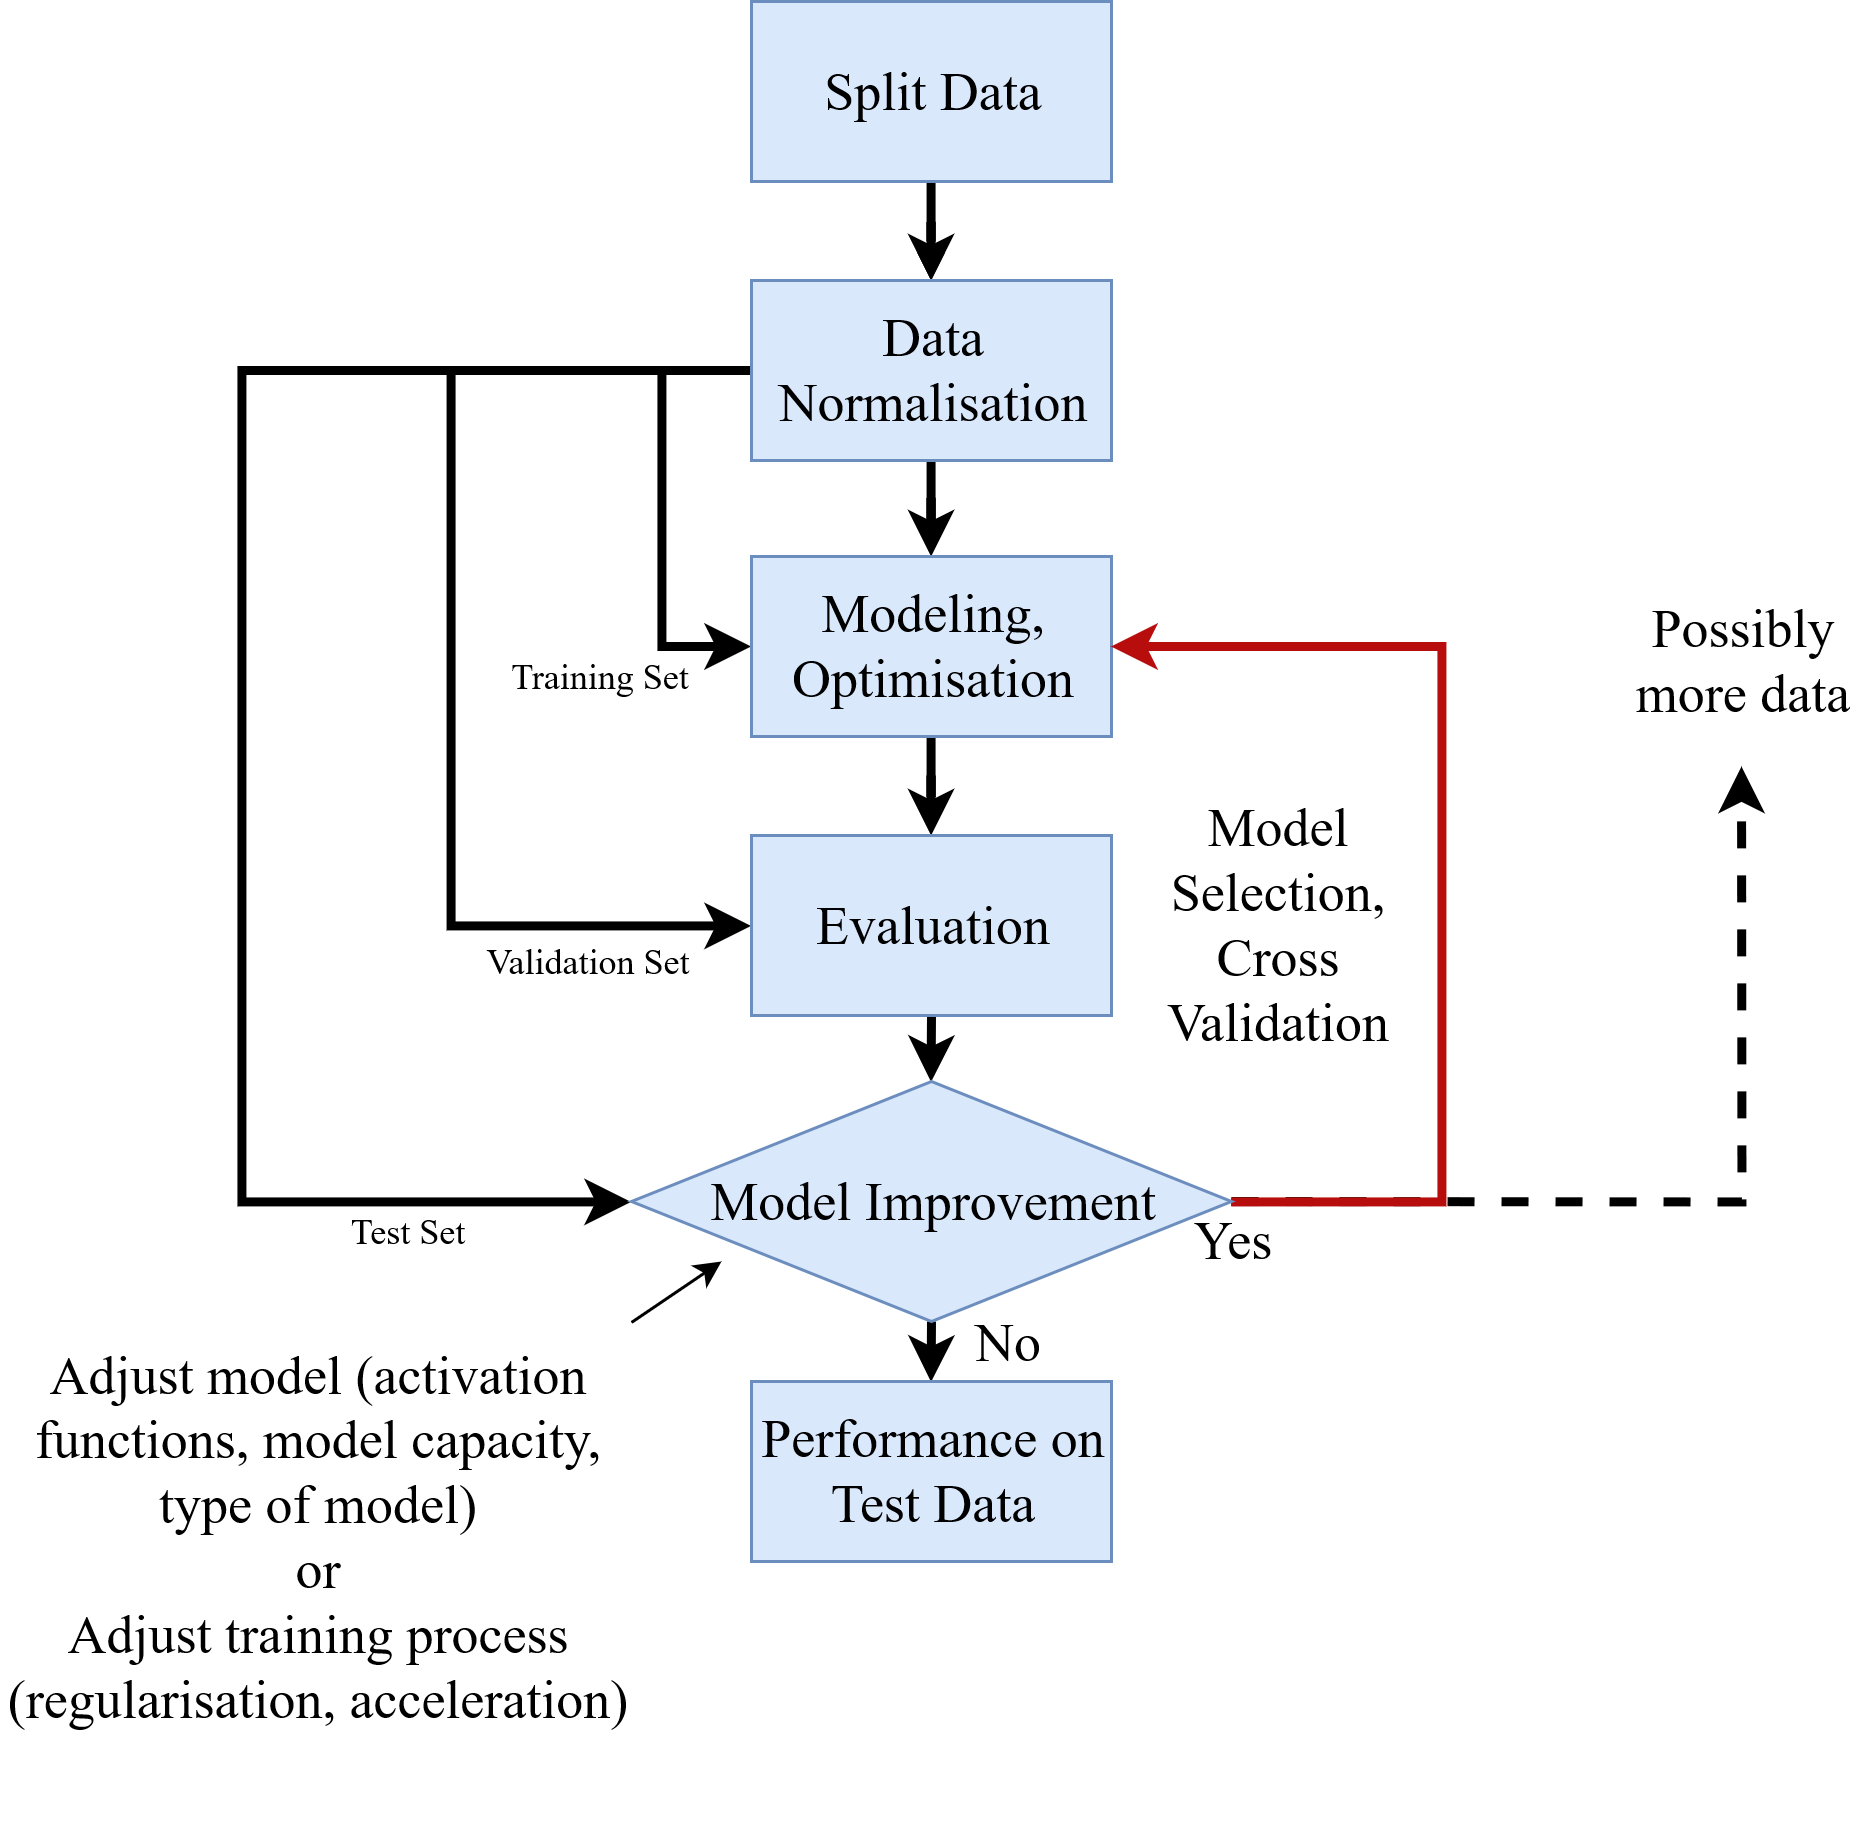
\includegraphics[width=0.6\linewidth]{img/standard_process_machine_learning}
	\caption{The general process used in Machine Learning}
	\label{fig:standardprocessmachinelearning}
\end{figure}

\subsection{k-fold Cross Validation}
Procedure for making efficient use of the data for more robust estimation of validation set performance, particularly useful if data is scarce.

\paragraph{Algorithm}
\begin{itemize}
	\item Randomly shuffle the dataset.
	\item Split dataset into test set ($D_{test}$) and the rest ($D_0$)
	\item Split $D_0$ into $k$ equally sized folds. \emph{Typical choice} $k = \{5,10\}$
	\item For each fold:
	\begin{itemize}
		\item Use the selected fold as validation set and the remaining folds as training set.
		\item Fit the model on the remaining folds.
		\item Evaluate the fitted model with the selected validation fold.
		\item Retain the evaluation score (performance)
	\end{itemize}
	\item Report the performance as average of retained evaluation scores.
\end{itemize}

\paragraph{Integrated into Model Selection Process}
\begin{itemize}
	\item Select the model, the hyper-parameters leading to the best performance
	\item Train with the combined training and validation set
	\item Report its performance on the basis of the test set
\end{itemize}

\begin{figure}[tbh]
	\centering
	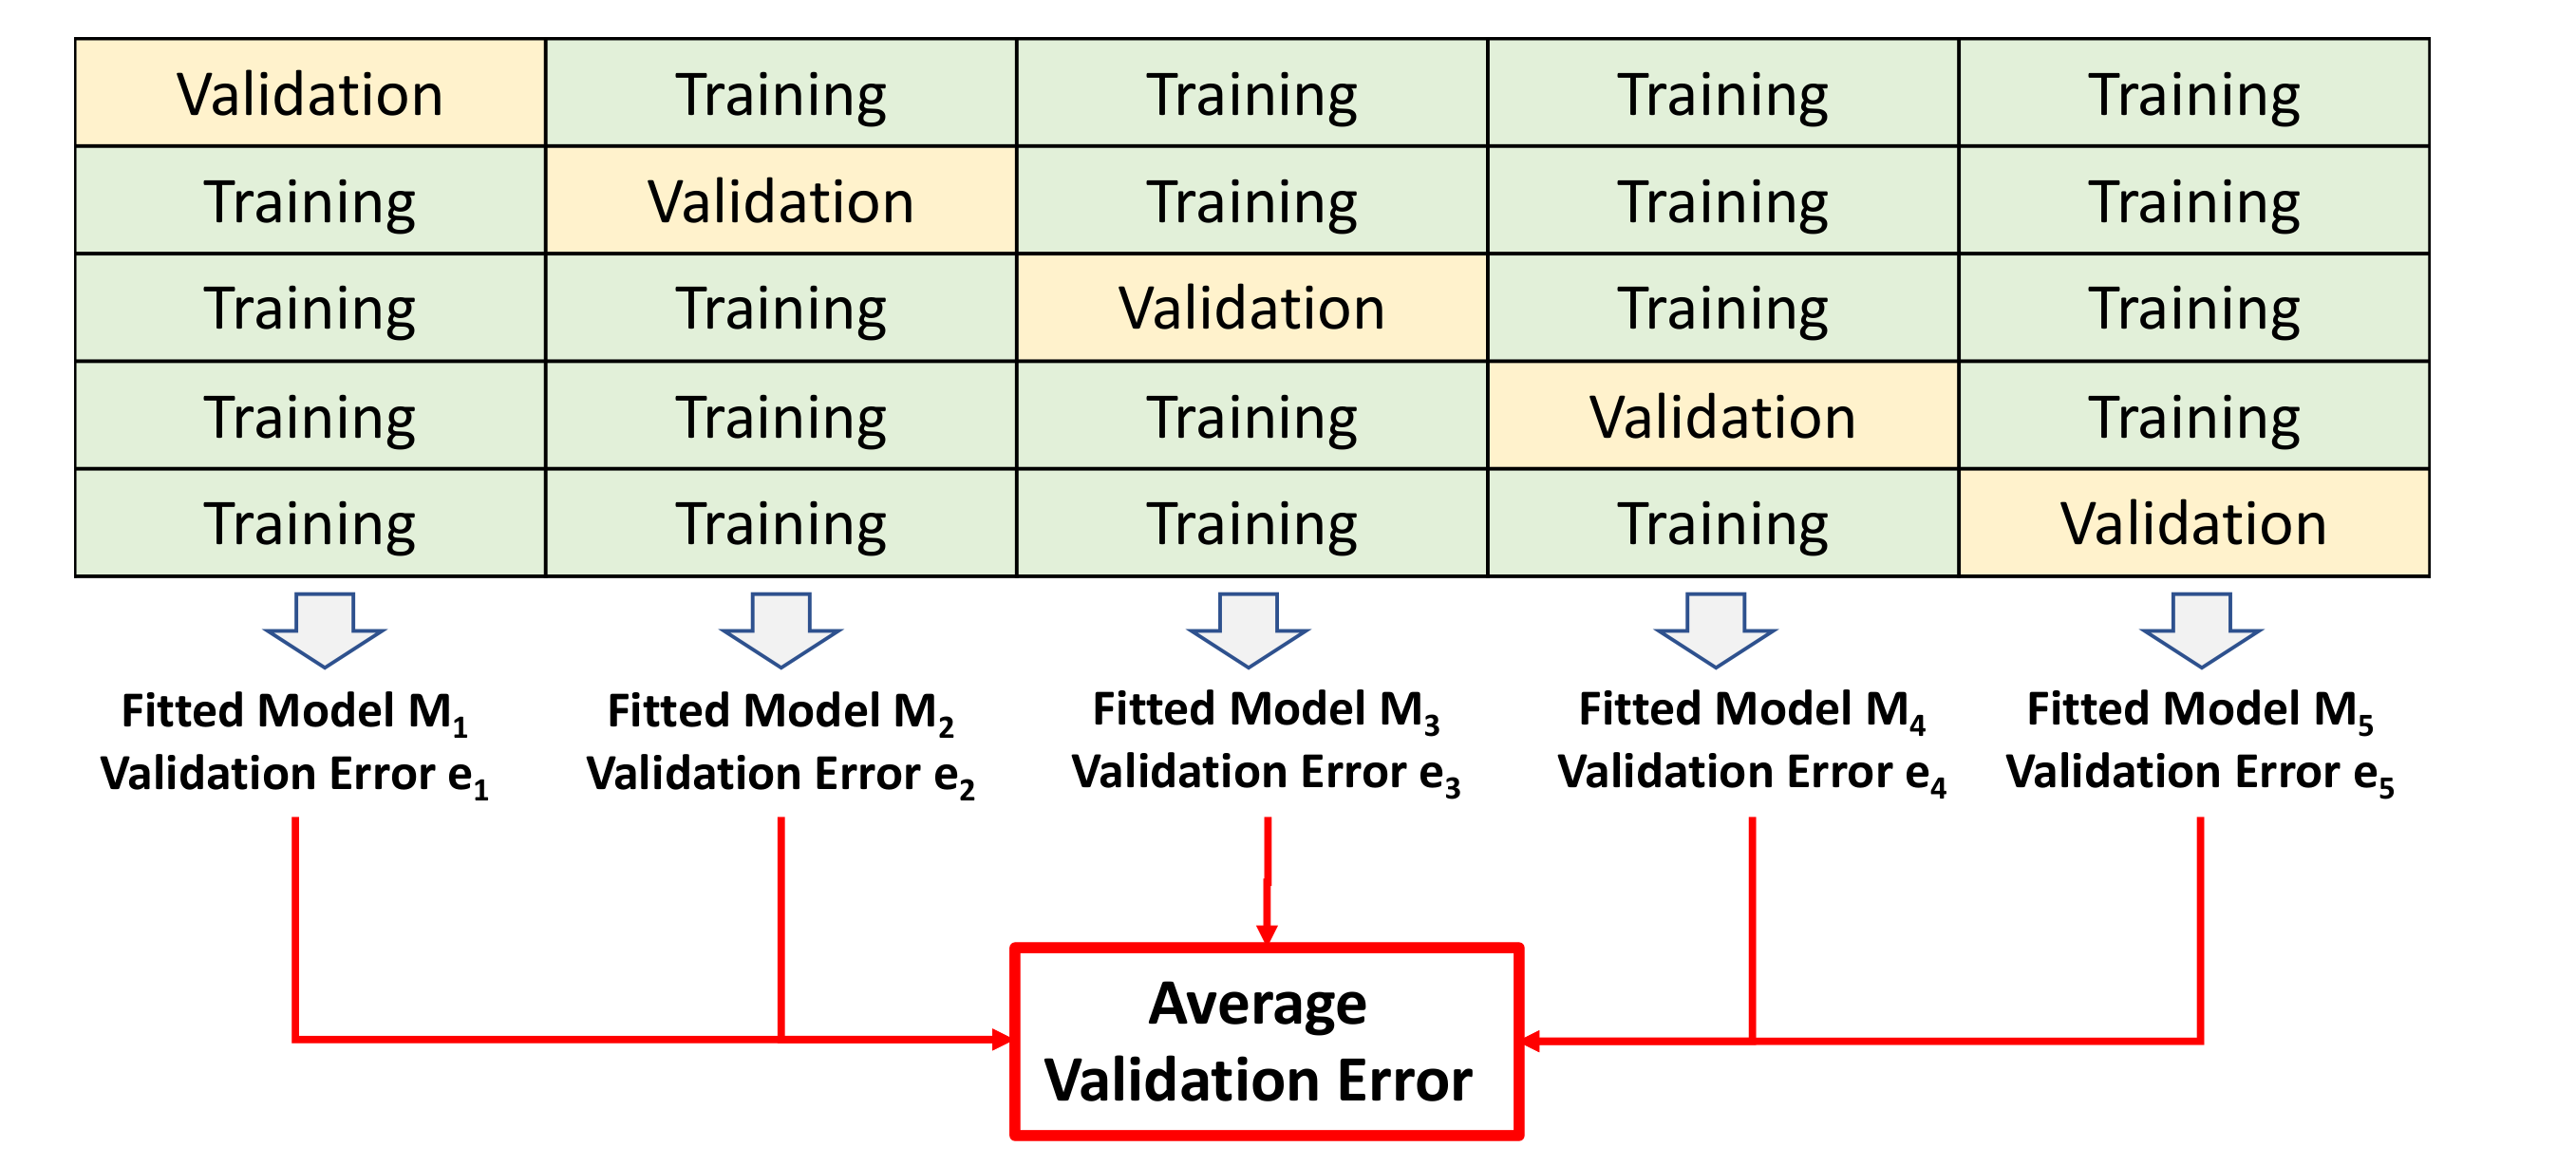
\includegraphics[width=0.8\linewidth, keepaspectratio]{k_fold_cross_validation}
	\caption{Visualisation of k-fold cross validation}
	\label{fig:kfoldcrossvalidation}
\end{figure}

\subsubsection{Benefits of Cross Validation}

\begin{figure}[H]
	\centering
	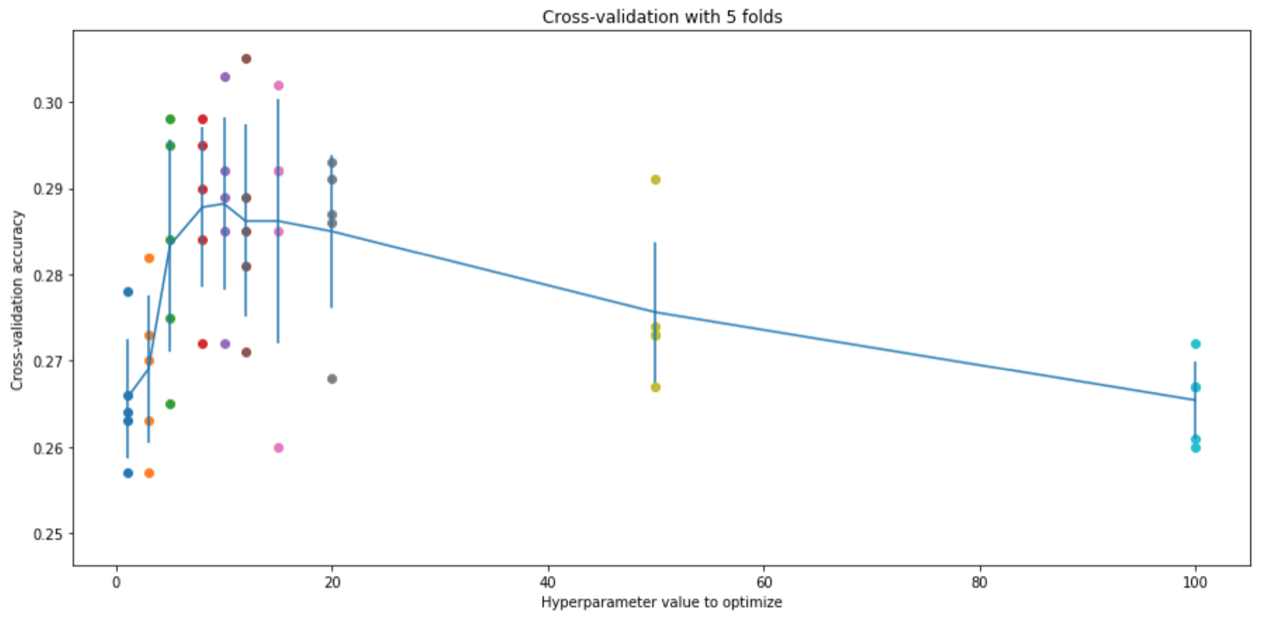
\includegraphics[width=0.6\linewidth]{img/k_fold_cross_validation_benefits}
\end{figure}

For selected hyper-parameter values, the performance for each of the five folds is computed. The spread on a given hyper-parameter value shows the sensitivity of the performance metric on the split of the data and it gives a feeling about the confidence of the performance estimates.

\section{Performance Measures}

\subsection{Confusion Matrix}

\begin{minipage}{0.5\textwidth}
	A confusion matrix measures the test performance of a classification system on a per-class basis by indicating the number of samples of actual class a predicted as class $b$. The rows relate to the actual class labels a and the columns to the predicted class labels $b$.
\end{minipage}
\begin{minipage}{0.5\textwidth}
	\centering
	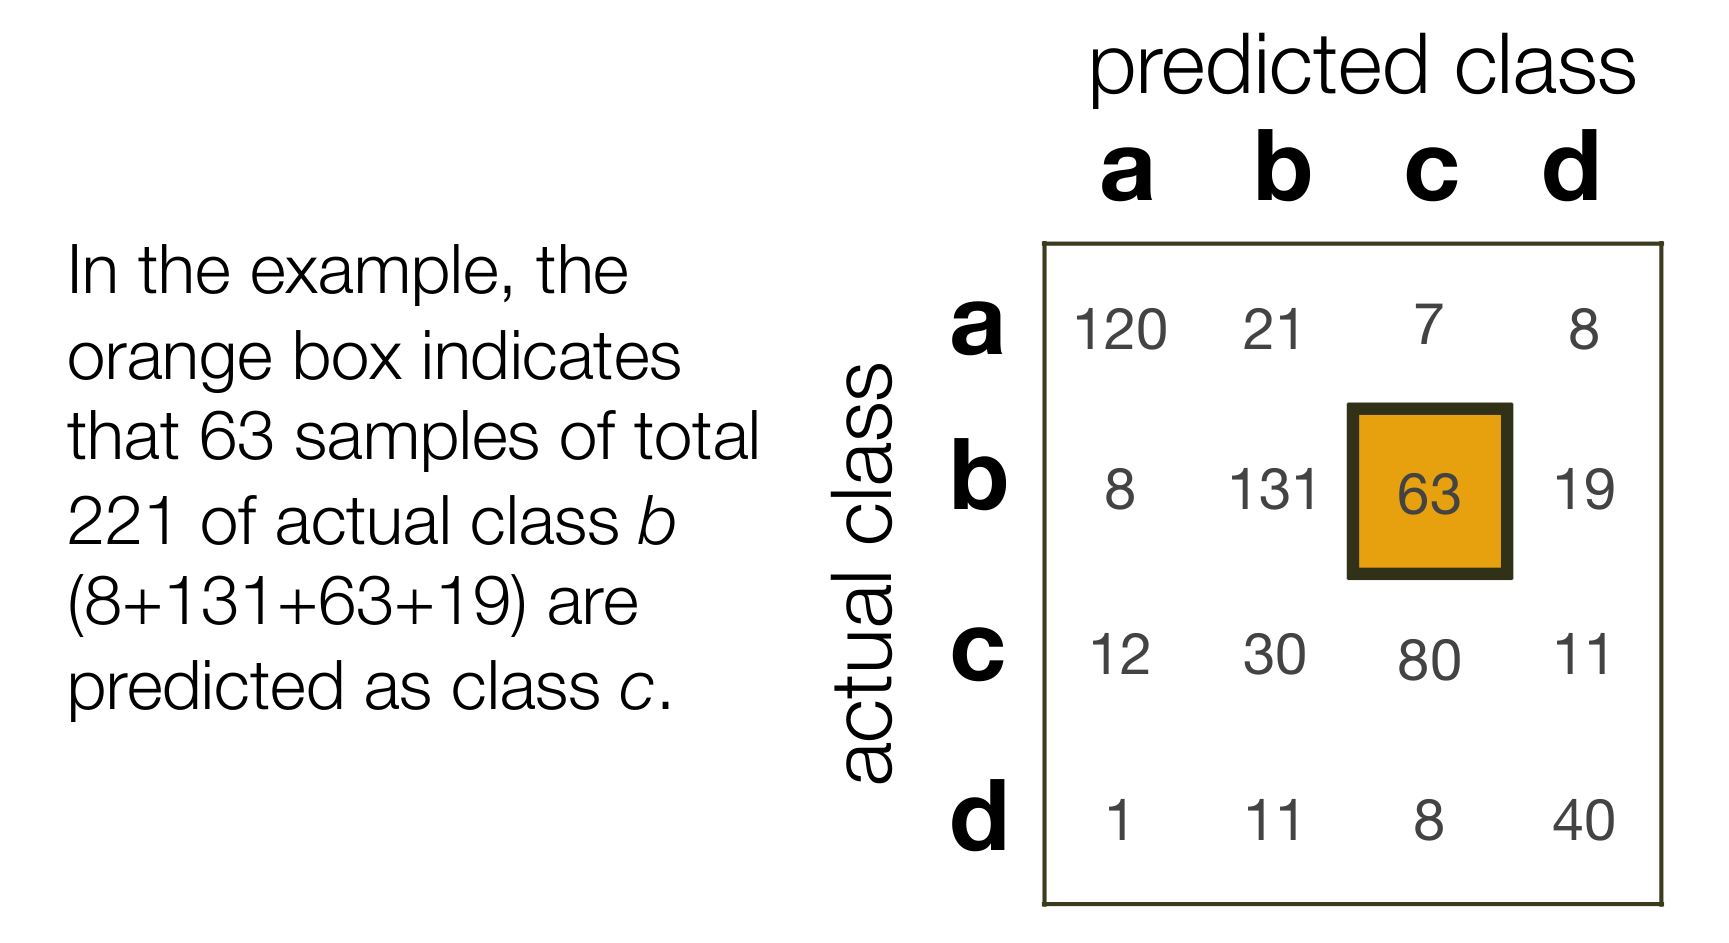
\includegraphics[width=\linewidth,keepaspectratio]{confusion_matrix}
\end{minipage}

\begin{minted}{python}
from sklearn.metrics import confusion_matrix

weights = params['W']
biases = params['b']

ypred_test = np.argmax(predict(weights, biases, x_test), axis=0)

conf_matrix = confusion_matrix(y_test.T, ypred_test.T)
\end{minted}

\begin{figure}[H]
	\centering
	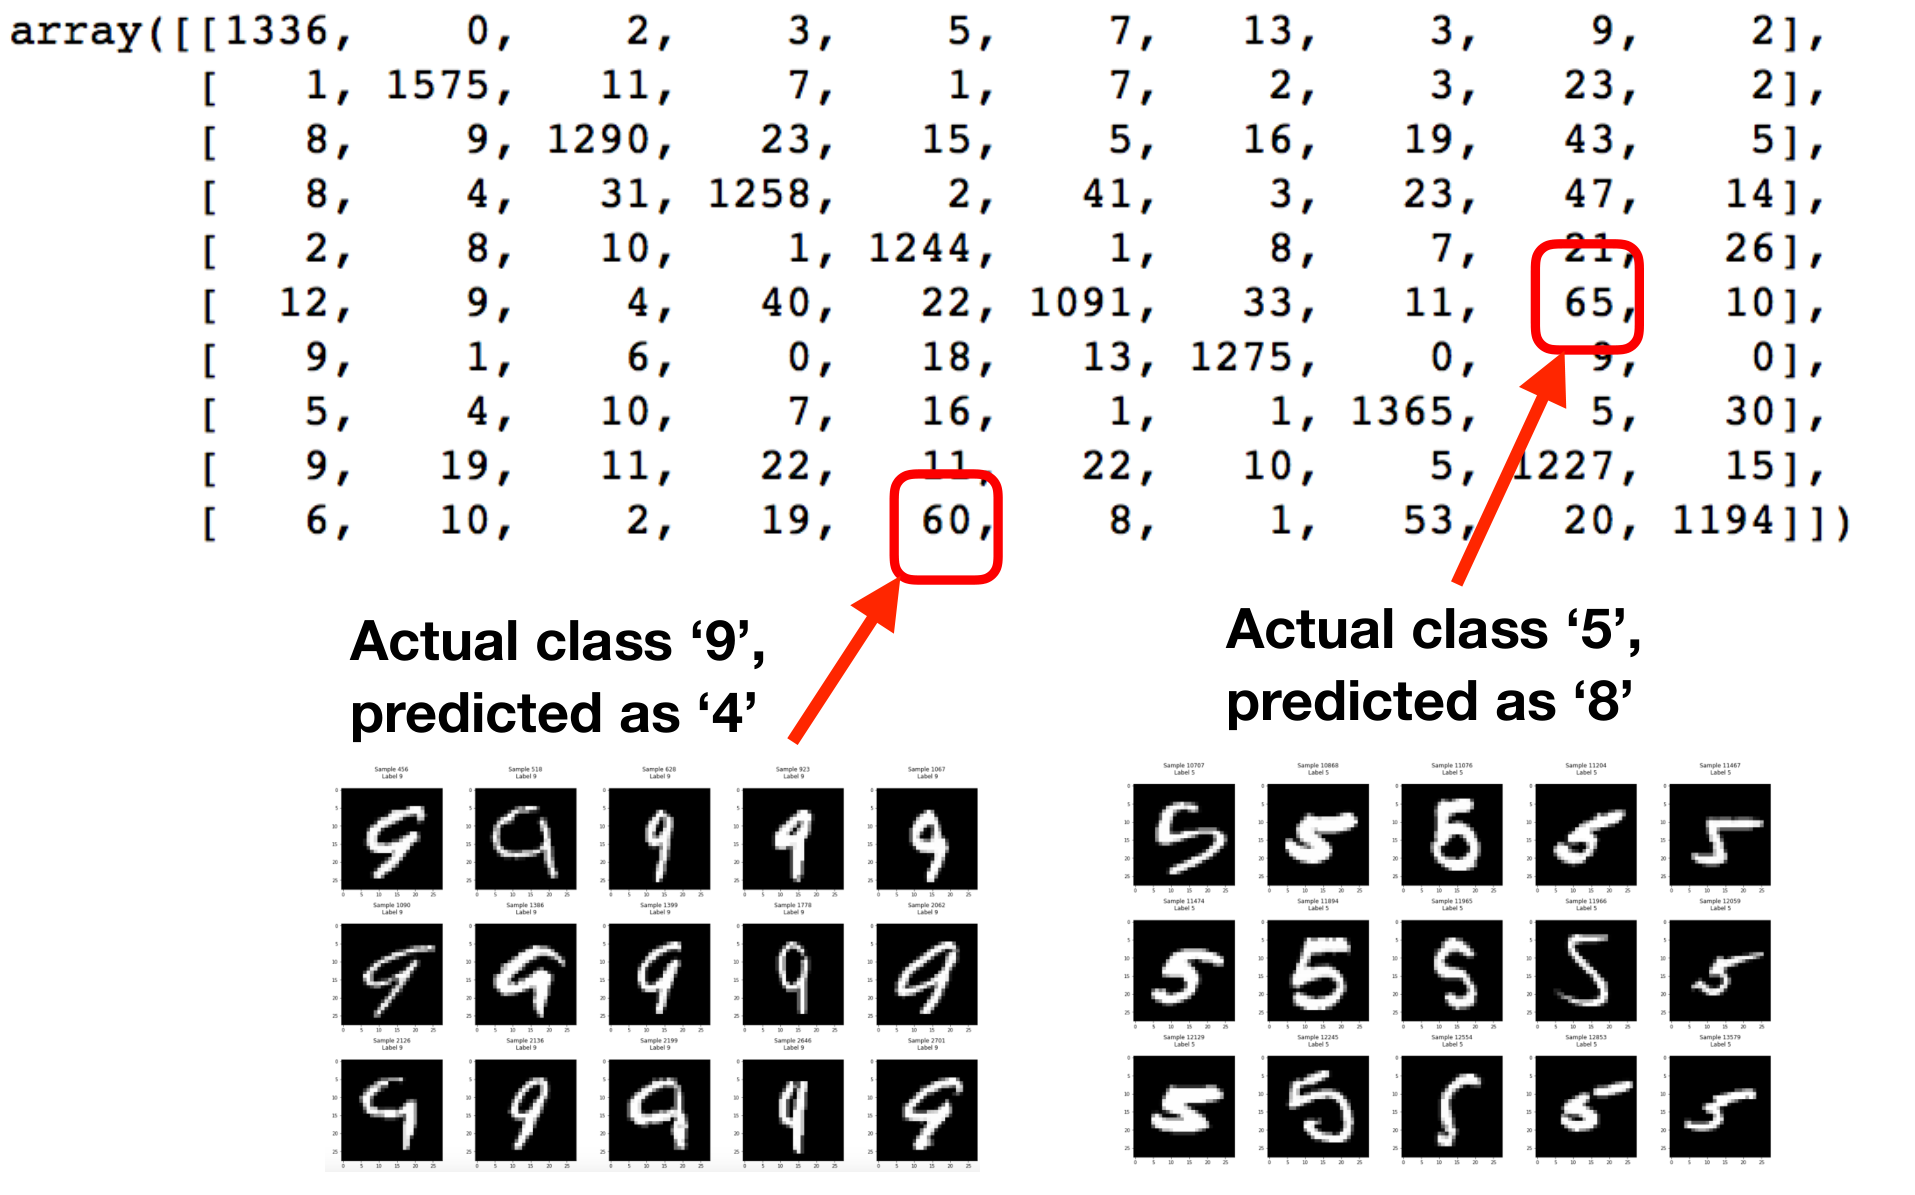
\includegraphics[width=0.8\linewidth,keepaspectratio]{confusion_matrix_output}
\end{figure}

\subsection{Overall Accuracy and Error Rate}

\paragraph{Accuracy} percentage of correct classifications
\begin{equation*}
	\text{accuracy} = \frac{\sum\text{diagonal elements}}{\text{number of samples}}
\end{equation*}

\paragraph{Error Rate} percentage of wrong classifications
\begin{equation*}
	\text{error rate} = 1 - \text{accuracy}
\end{equation*}

\subsection{Confusion Table}

A \textbf{confusion table} is used to measure the classification performance of a two-class system.

\begin{figure}[H]
	\centering
	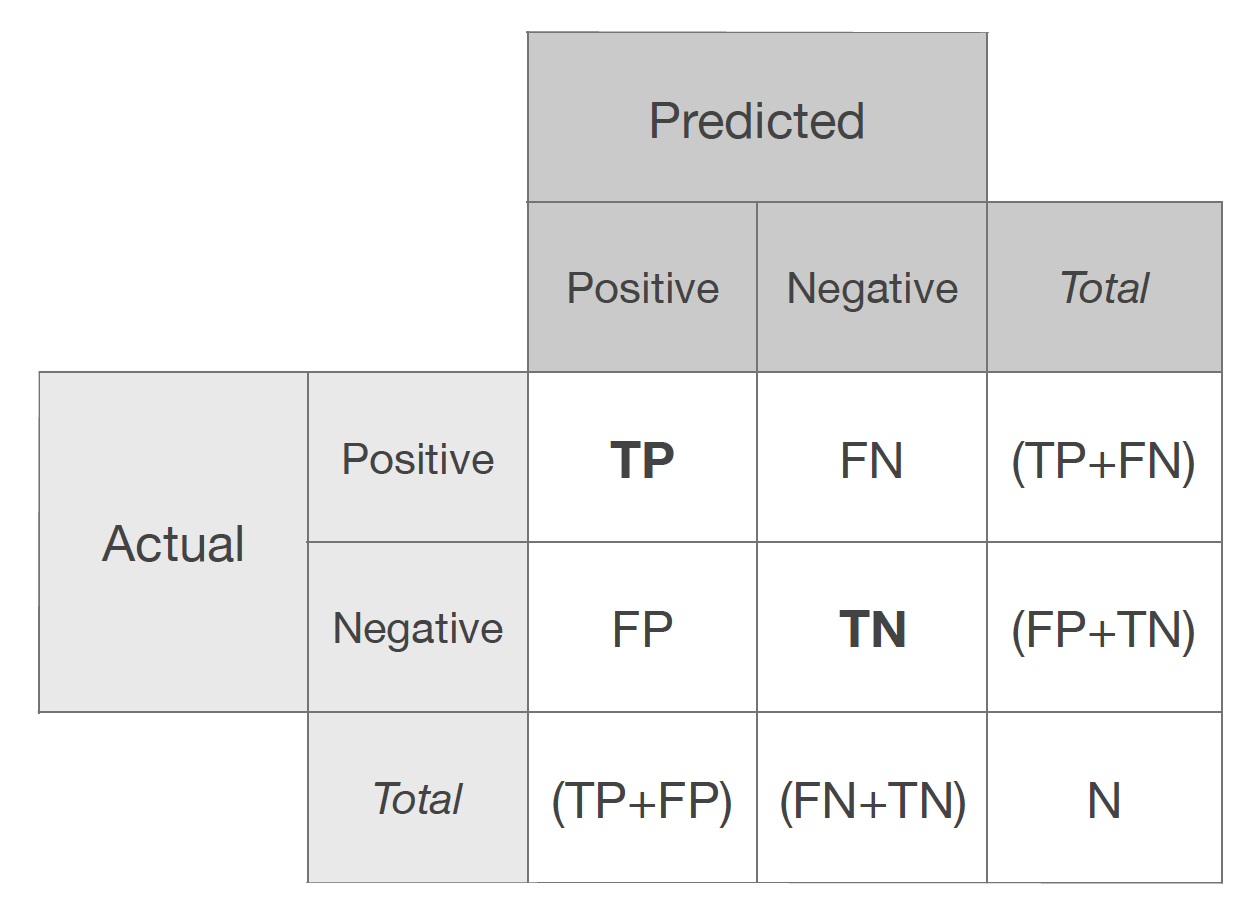
\includegraphics[width=0.4\linewidth]{img/confusion_table}
\end{figure}

\subsection{Class Accuracy}

\begin{minipage}{0.5\textwidth}
	\paragraph{Class Accuracy} percentage of correct classifications considering a given class against the others
	\begin{equation*}
		\frac{TP + TN}{Total}
	\end{equation*}
\end{minipage}
\begin{minipage}{0.5\textwidth}
	\centering
	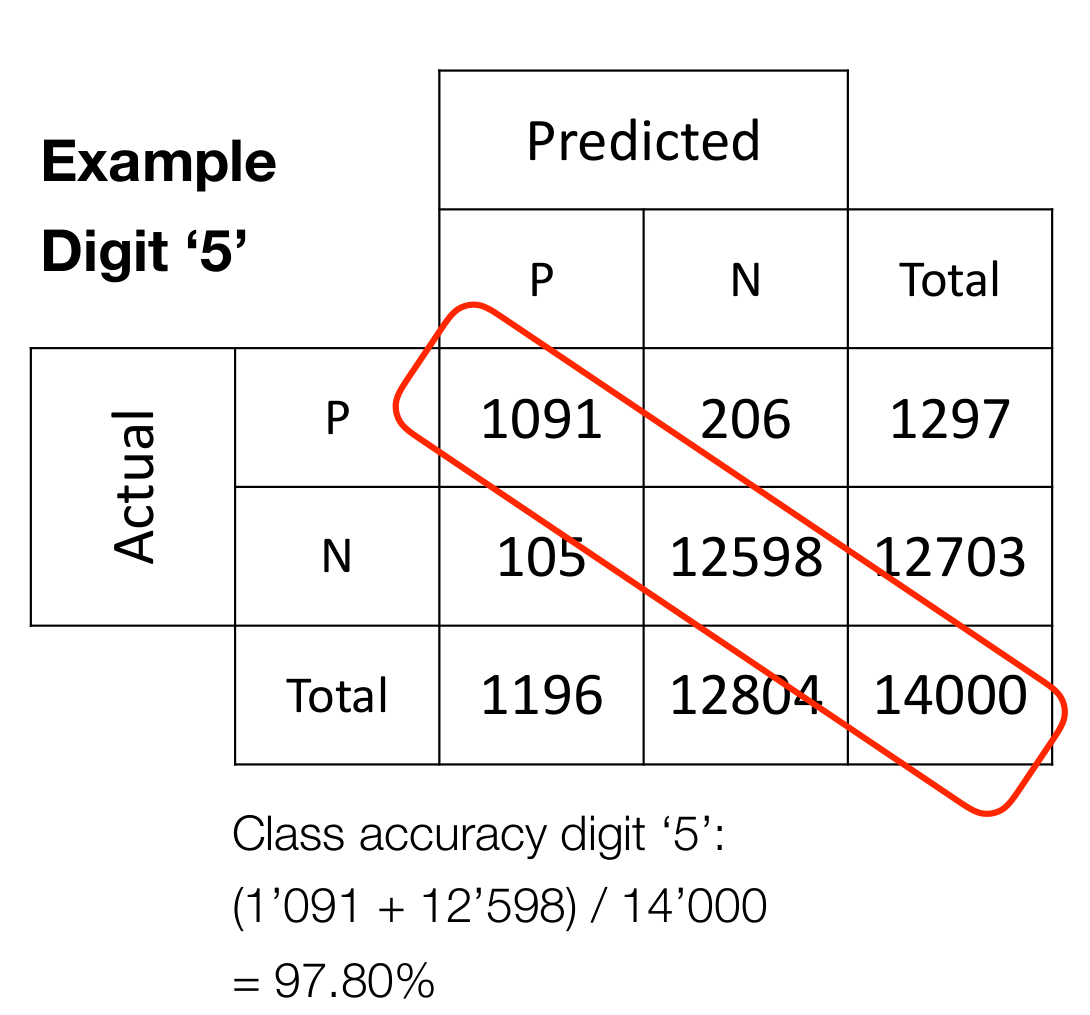
\includegraphics[width=0.8\linewidth,keepaspectratio]{class_accuracy}
\end{minipage}

\subsection{Per Class Sensitivity or Recall}

\begin{minipage}{0.5\textwidth}
	\paragraph{Class Sensitivity or Recall} percentage of correct classification for a given class
	\begin{equation*}
	\frac{TP}{TP+FN}
	\end{equation*}
\end{minipage}
\begin{minipage}{0.5\textwidth}
	\centering
	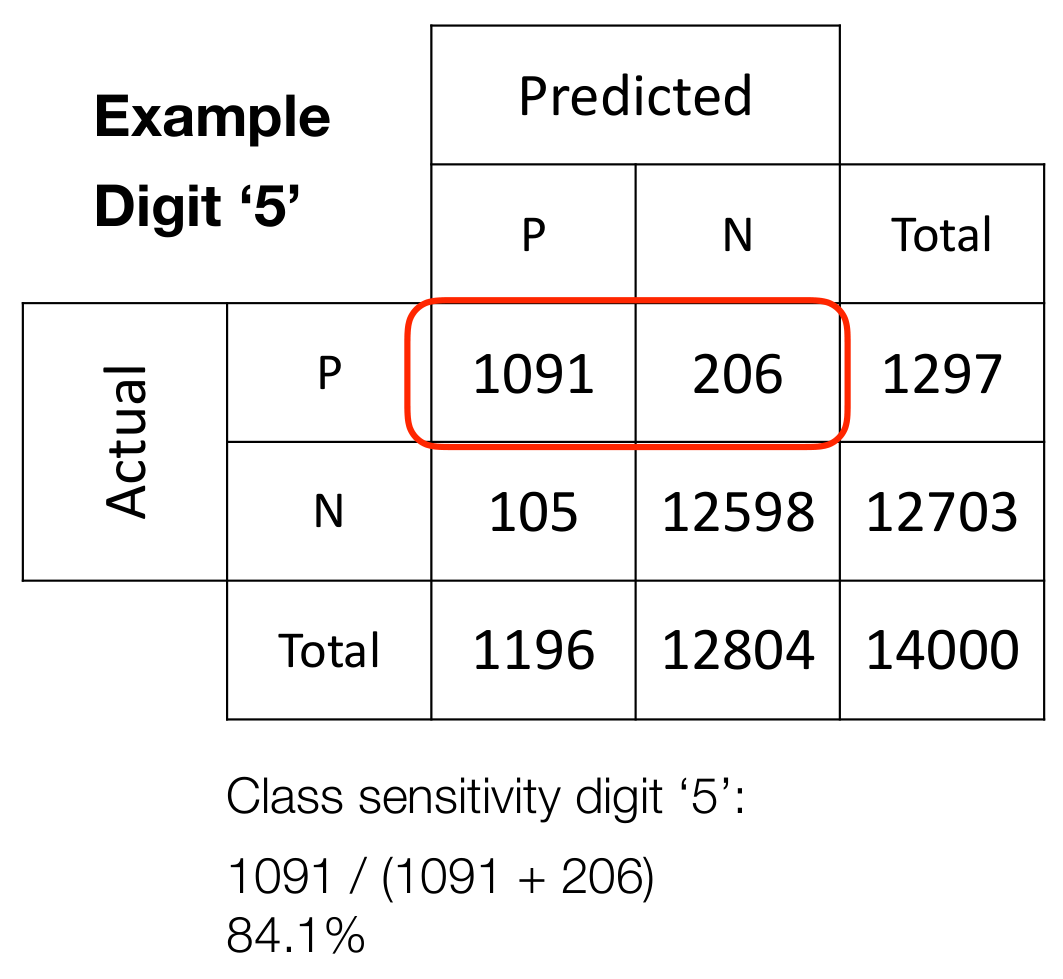
\includegraphics[width=0.8\linewidth,keepaspectratio]{class_recall}
\end{minipage}

\subsection{Class Precision}

\begin{minipage}{0.5\textwidth}
	\paragraph{Class Precision} percentage of correct classification in the predicted outputs for a given class
	\begin{equation*}
	\frac{TP}{TP+FP}
	\end{equation*}
\end{minipage}
\begin{minipage}{0.5\textwidth}
	\centering
	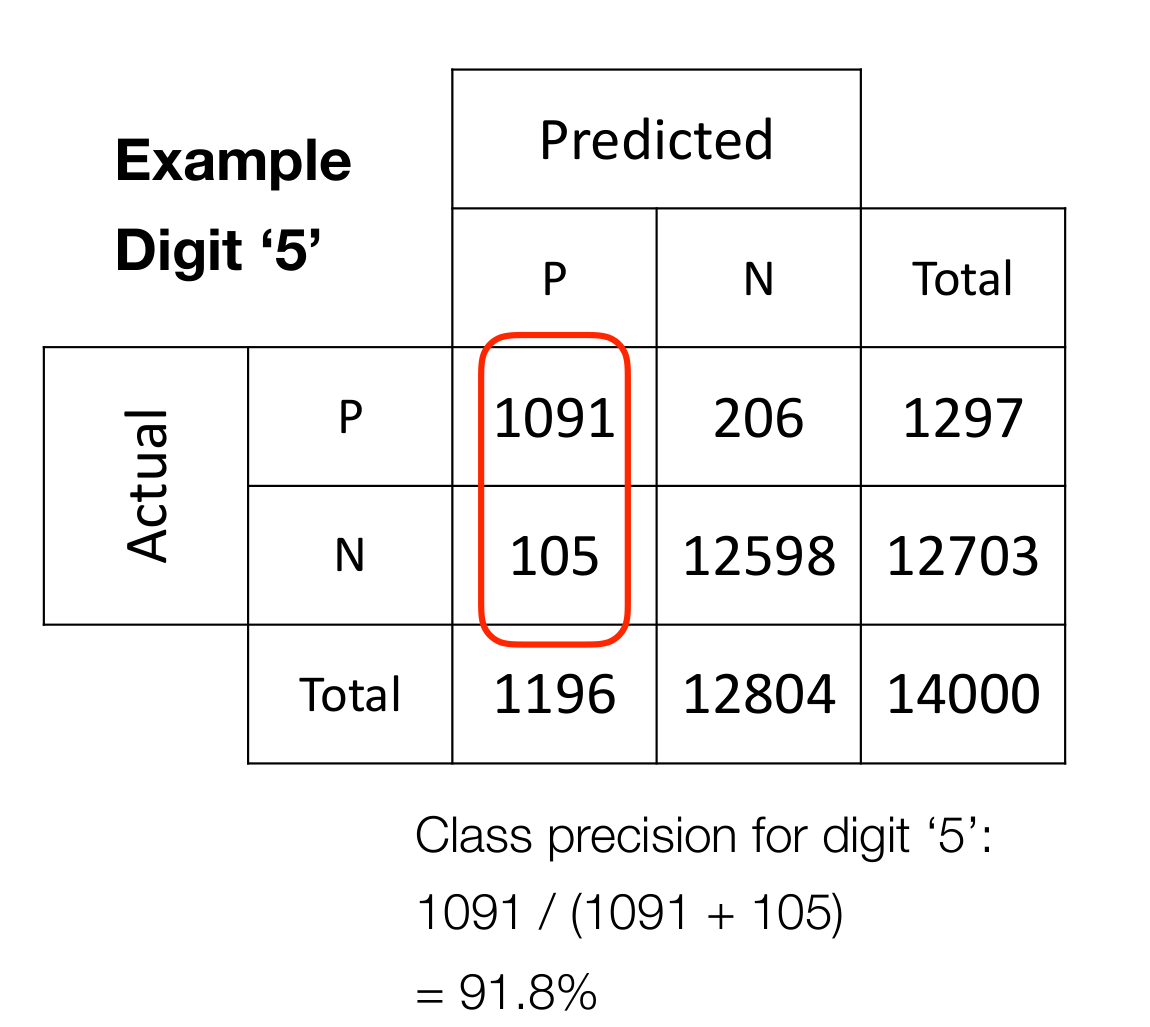
\includegraphics[width=0.8\linewidth,keepaspectratio]{class_precision}
\end{minipage}

\subsection{F-Score}

\begin{minipage}{0.5\textwidth}
	\paragraph{F-Score or F1-Score} harmonic mean of recall and precision
	\begin{equation*}
	\frac{1}{\frac{1}{2}\left(\frac{1}{\text{recall}} + \frac{1}{\text{precision}} \right)} = \frac{TP}{TP + \frac{FP + FN}{2}}
	\end{equation*}
\end{minipage}
\begin{minipage}{0.5\textwidth}
	\centering
	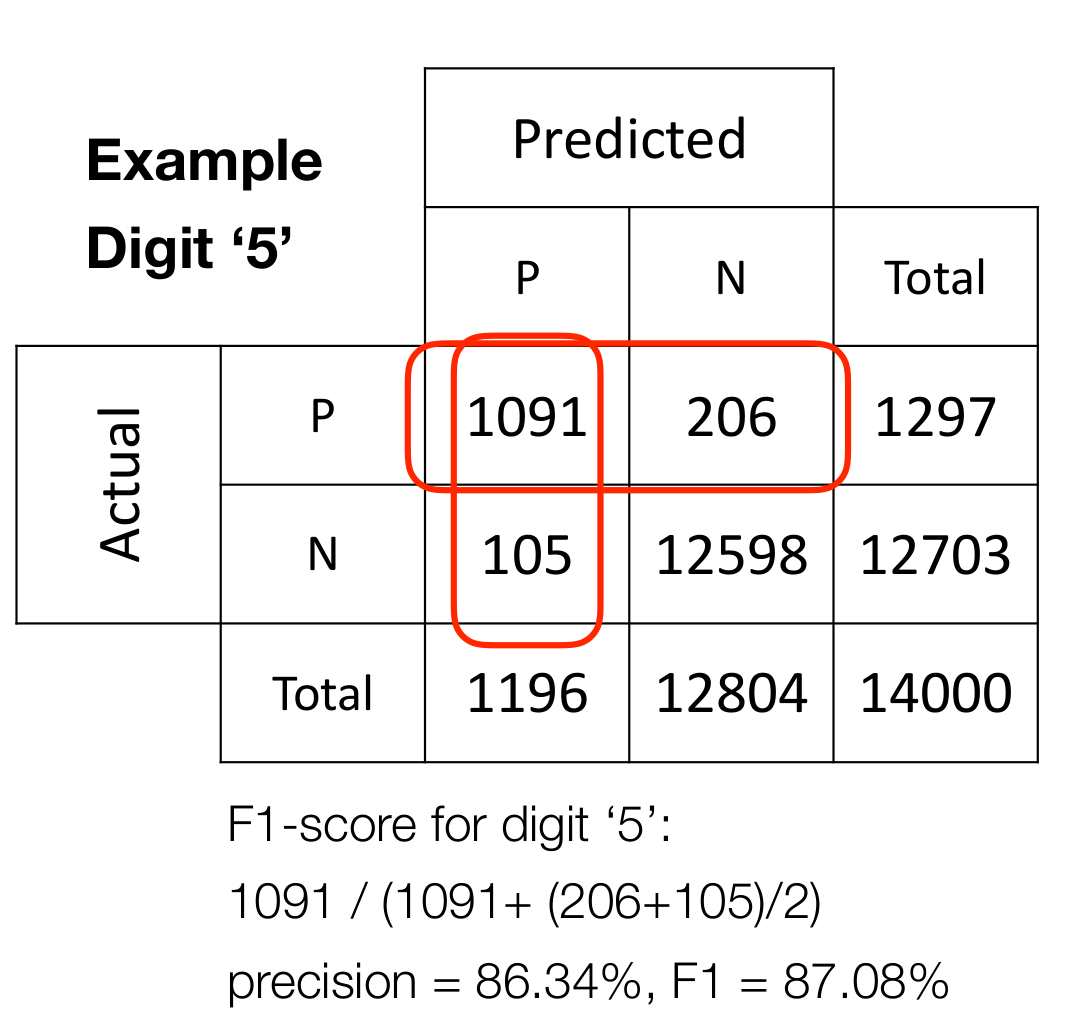
\includegraphics[width=0.8\linewidth,keepaspectratio]{f1_score}
\end{minipage}

\subsection{System Performance Metrics}
\noindent
\begin{minipage}{\textwidth}
	\renewcommand{\arraystretch}{1.5}
	\centering
	\begin{tabularx}{\linewidth}{|l|X|}
		\hline
		\textbf{System Accuracy} & Average Class Accuracy\\
		\hline
		\textbf{System Recall} & Average Class Recall\\
		\hline
		\textbf{System Precision} & Average Class Precision\\
		\hline
		\textbf{System F1-Score} & Harmonic Mean of System Precision and System Recall\\
		\hline
	\end{tabularx}
\end{minipage}

\section{Curse of Dimensionality}

In classical machine learning there is a local smoothness assumption of the function the model tries to learn. This means that this function does not vary much locally and stays approximately constant in small regions. This assumption allows to generalise to variations in small regions from closely located training examples. Training examples are needed in all the regions of interest. If no or only few examples are available in a given region, no confident predictions can be made. This assumption works fine if the dimensionality of the data is not too high, but fails in typical Deep Learning applications when dealing with image, speech or language data.

"...when the dimensionality increases, the volume of the space increases so fast that the available data become sparse. This sparsity is problematic for any method that requires statistical significance. In order to obtain a statistically sound and reliable result, the amount of data needed to support the result often grows exponentially with the dimensionality."

\subsection{Representation of Variational Characteristics}
Goal is to find a good representation for the variational characteristics observed in the data as needed by the underlying task. Typically, the patterns found in the data and its variational degrees of freedom are expected to be well represented on a much lower dimensional manifold.

\begin{theorem}
	The \textbf{core idea in Deep Learning} is
	\begin{itemize}
		\item the assumption that the data was generated by the composition of factors or features, potentially at multiple levels in a hierarchy
		\item learning involves discovering a set of underlying factors of variation that can be described in terms of other, simpler underlying factors arranged in a hierarchy
	\end{itemize}
\end{theorem}

\section{Computational Graphs}
A computational graph is a directed graph where
\begin{itemize}
	\item nodes correspond to operations or input variables
	\item edges correspond to inputs of an operation which can originate from input variables or outputs of other operations.
\end{itemize}

\noindent
Two types of input variables: Input data and model parameters.

\begin{figure}[tbh]
	\centering
	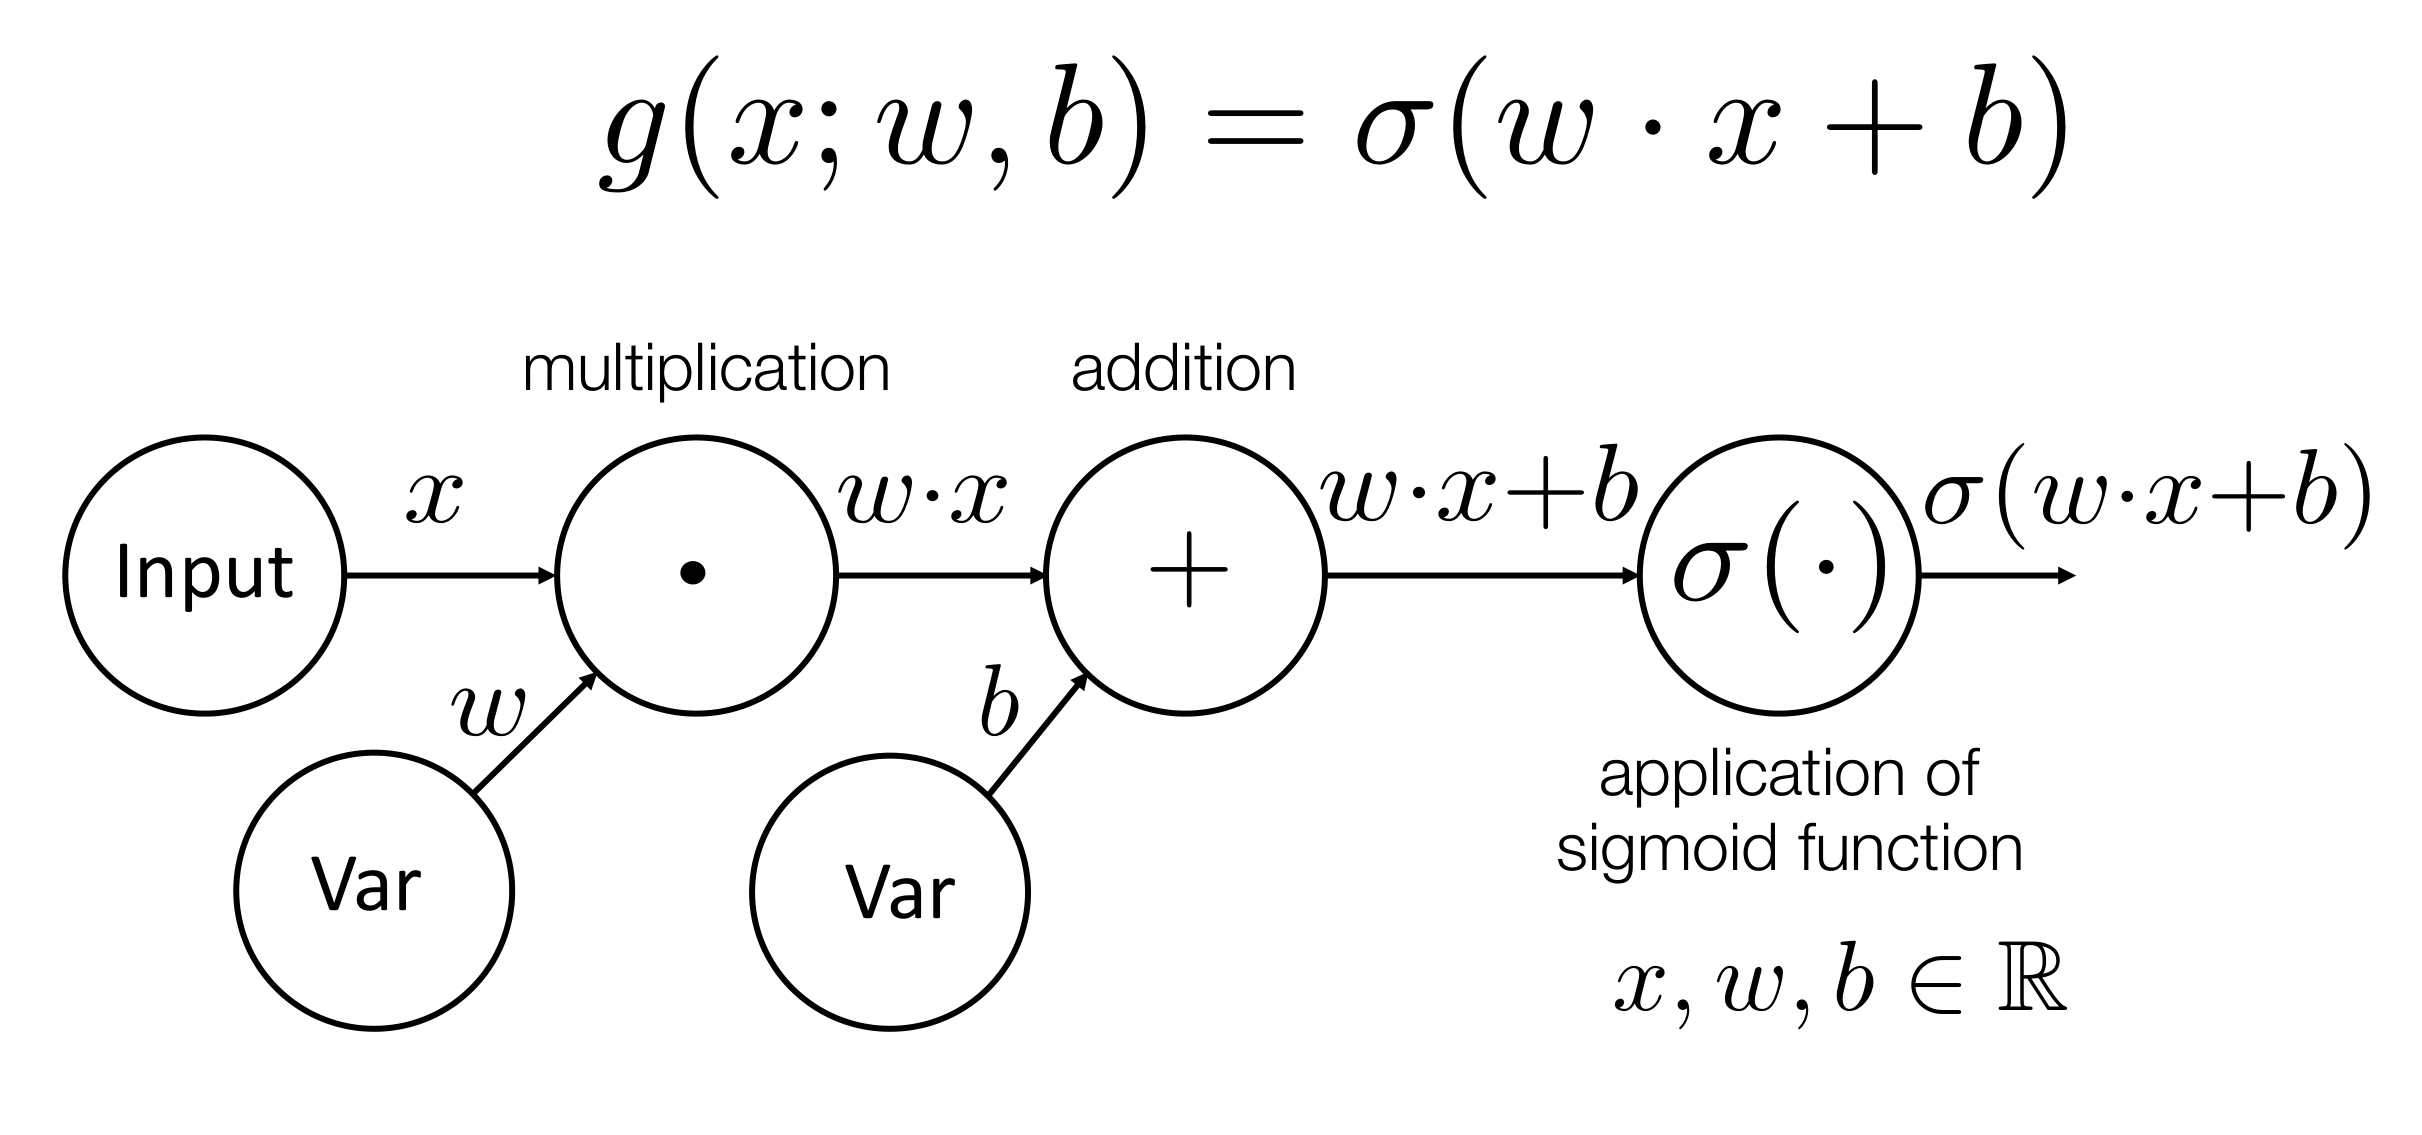
\includegraphics[width=0.6\linewidth]{computational_graph}
	\caption{Example of a computational graph}
	\label{fig:computationalgraph}
\end{figure}

Neural networks can be considered as a special form of computational graphs. Inputs into and outputs out of the nodes are multi-dimensional arrays called \emph{tensors}: scalars, 1d vectors, 2d matrices and higher rank objects.

\begin{figure}[tbh]
	\centering
	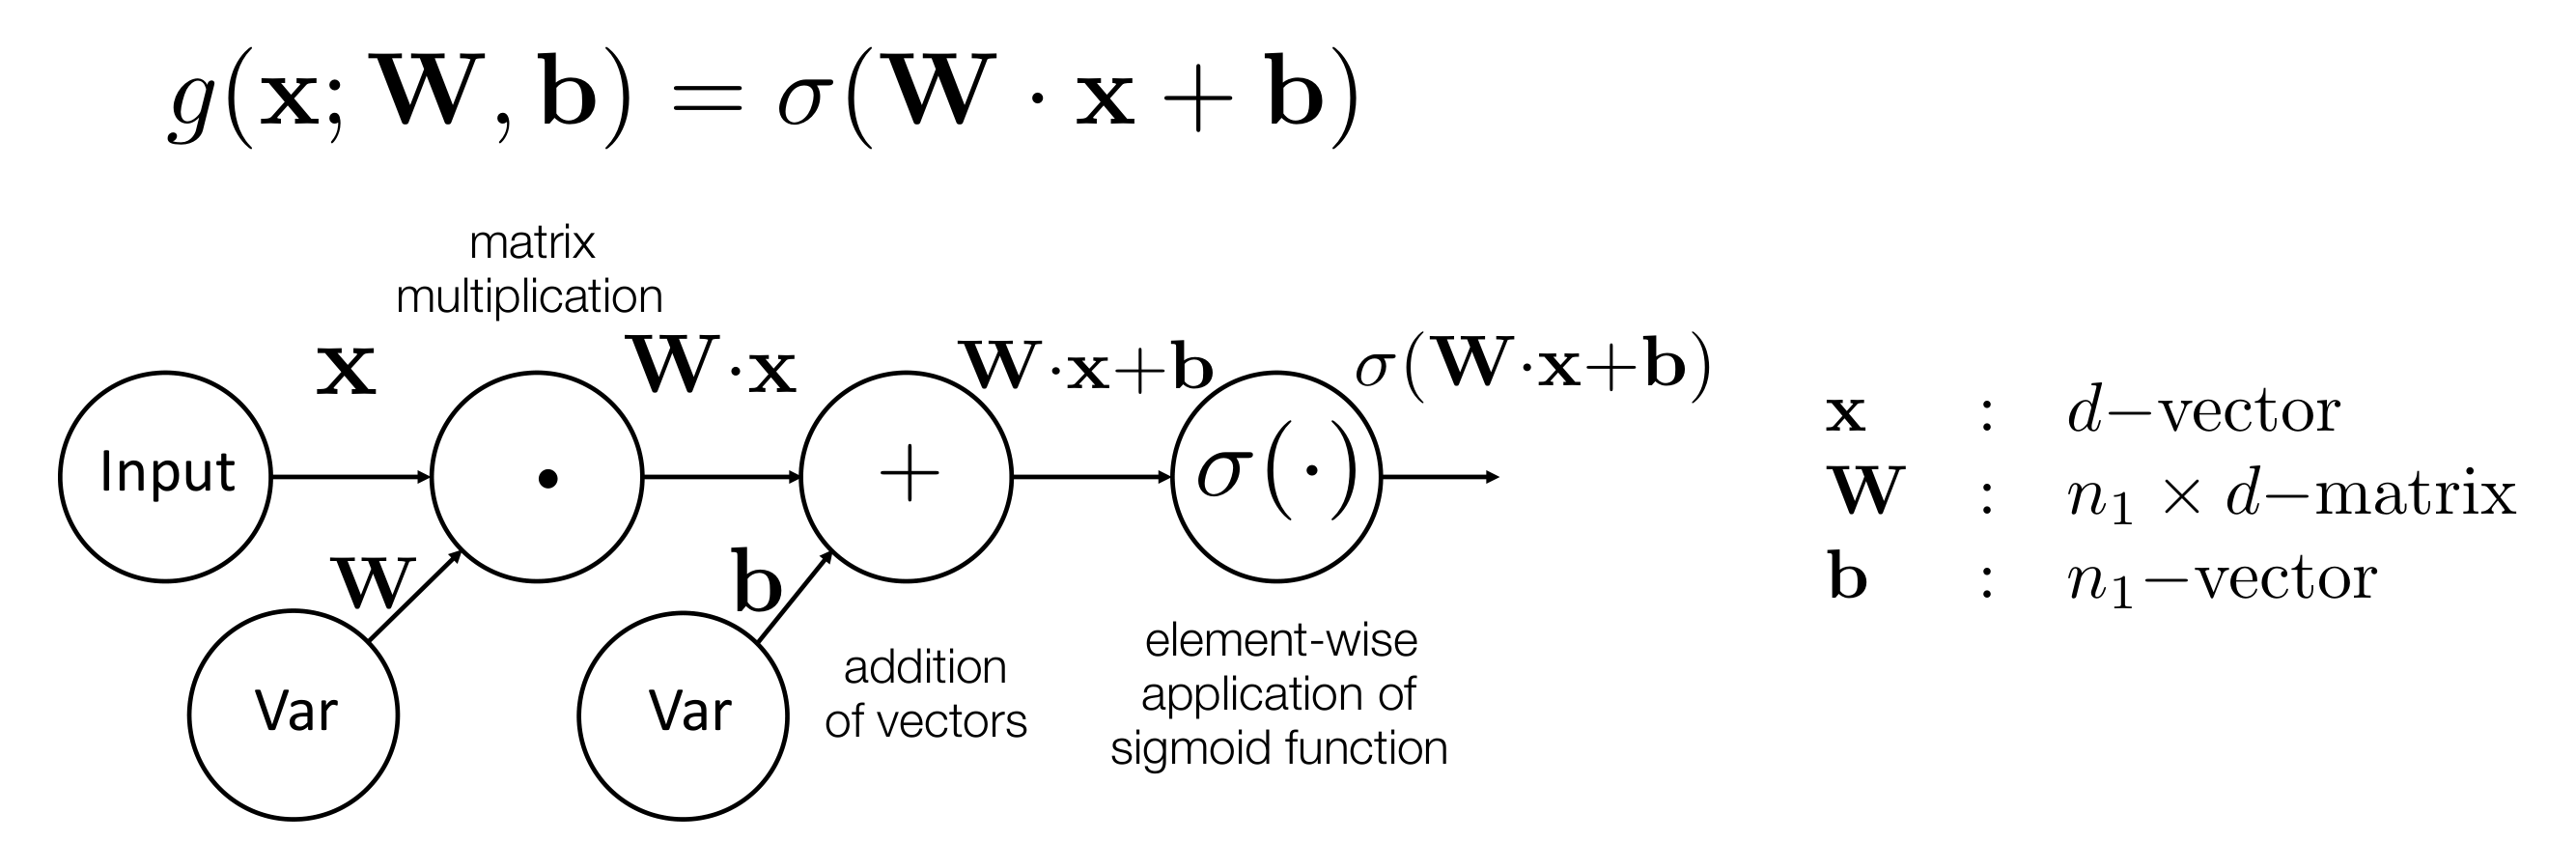
\includegraphics[width=0.6\linewidth]{img/computational_graph_output_layer}
	\caption{Computational graph for a network with just an output layer}
	\label{fig:computationalgraphoutputlayer}
\end{figure}

The operations of a single layer (affine transformation and application of activation function) can be collapsed into a single node. Layers are the abstraction level most Deep Learning frameworks use to define the architecture of a Deep Learning model.

\begin{minted}{python}
import tensorflow as tf
mnist = tf.keras.datasets.mnist

(x_train, y_train), (x_test,y_test) = mnist.load_data()
x_train, x_test = x_train/255.0, x_test/255.0

model = tf.keras.models.Sequential(
	[
		tf.kears.layers.Flatten(input_shape = (28,28)),
		tf.kears.layers.Dense(512, activation=tf.nn.relu),
		tf.kears.layers.Dropout(0.2),
		tf.kears.layers.Dense(10, activation=tf.nn.softmax)
	]
)
\end{minted}

\subsection{Multi-Layer Perceptron}
Represents function that computes from a sample $\textbf{x}^{(i)}$ of $n_x = n_0$ input features (represented by an $n_x$-vector) an output vector $\widehat{\textbf{y}}^{(i)}$.

\begin{figure}[H]
	\centering
	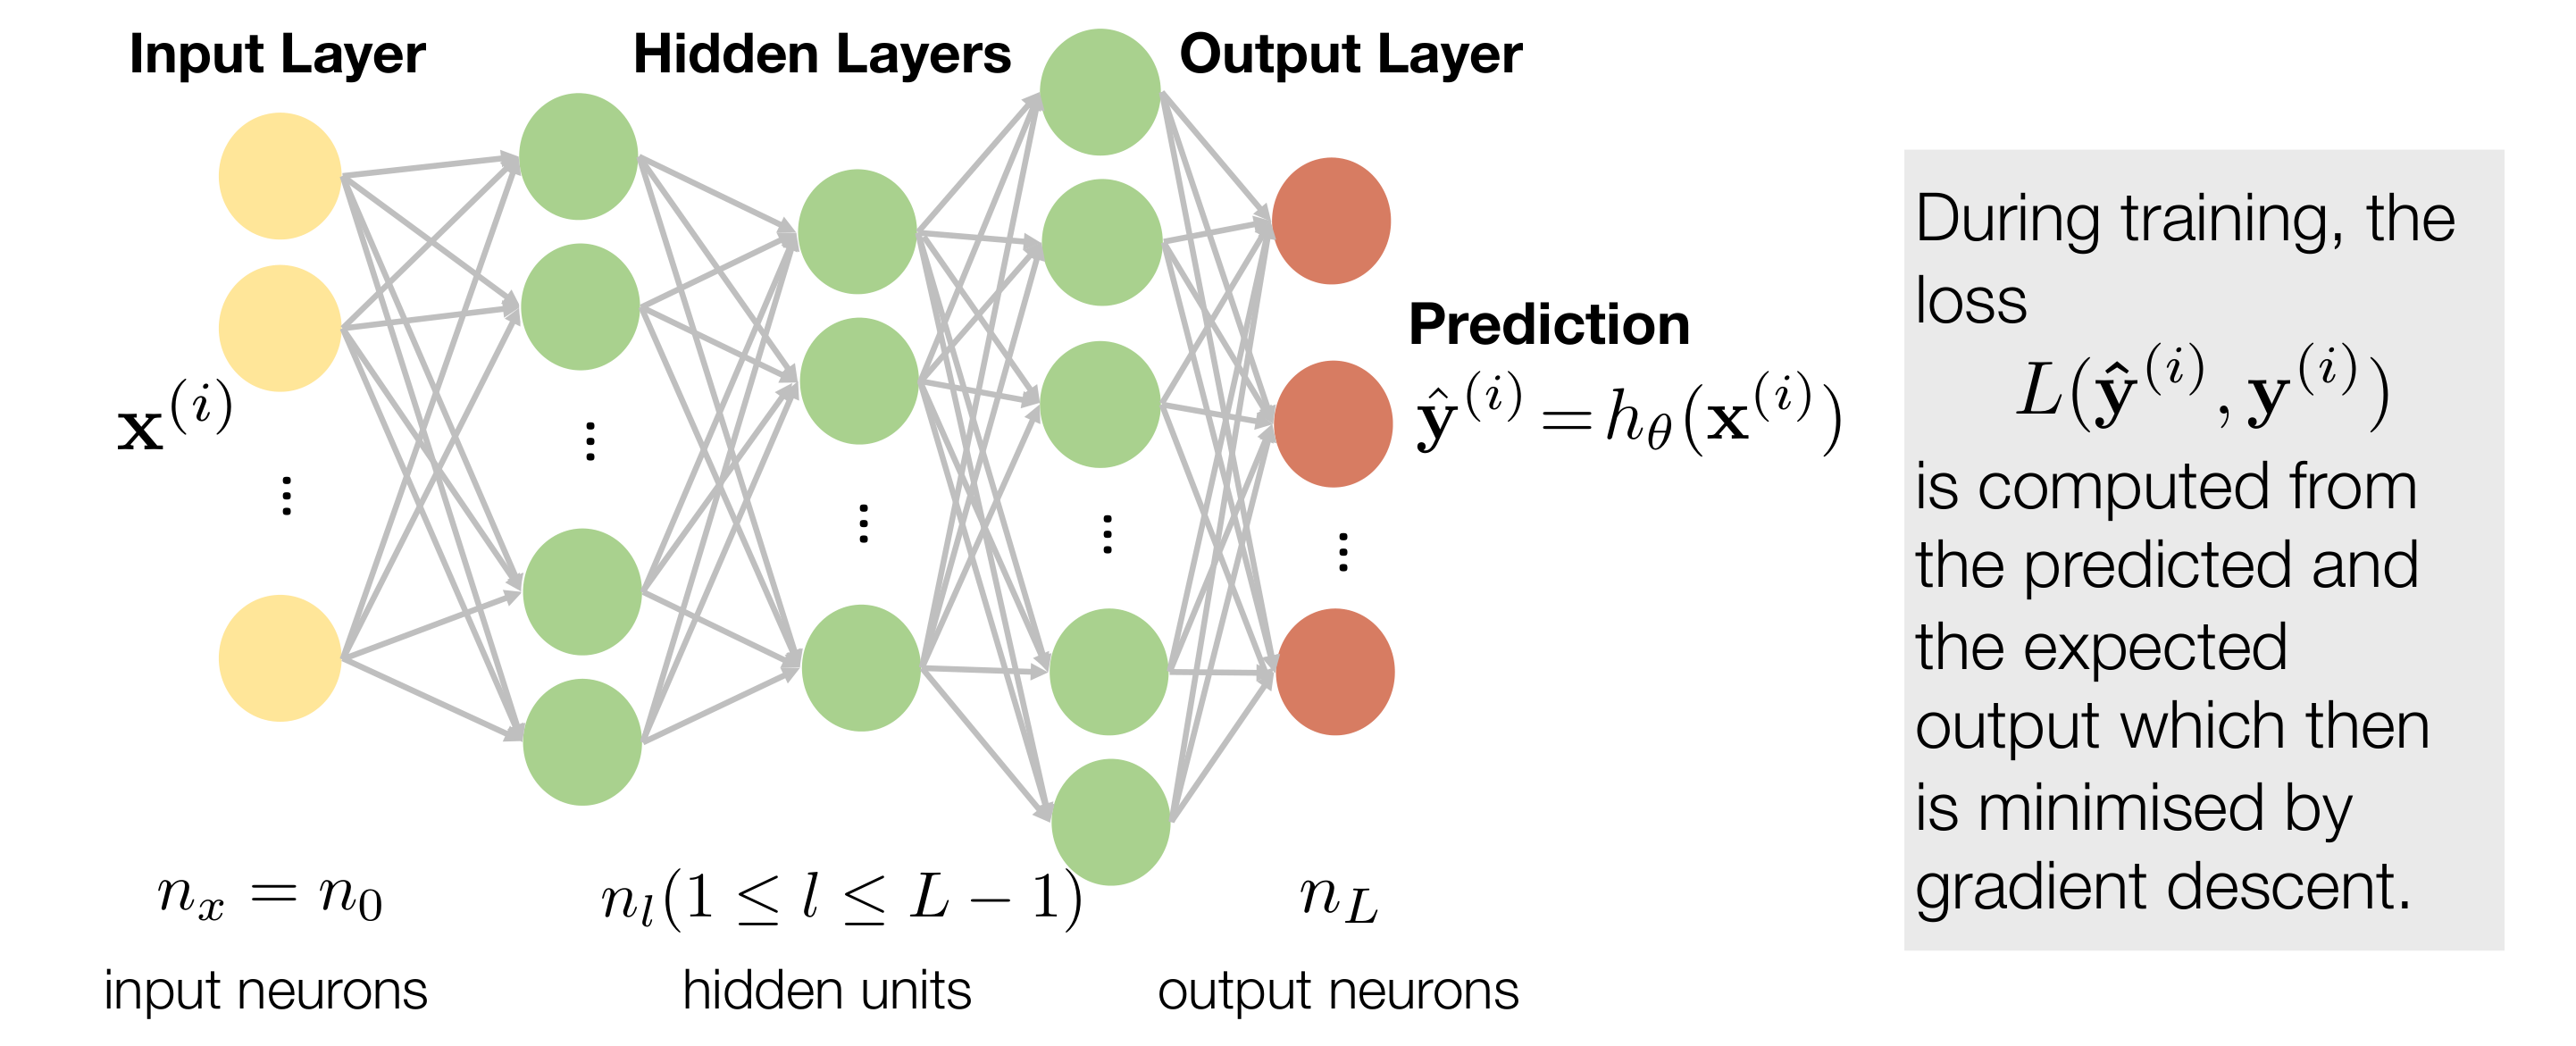
\includegraphics[width=0.8\linewidth]{mlp_graph}
	\caption{The nodes represent neural units which operate on output originating from many other units and produce scalar output}
	\label{fig:mlpgraph}
\end{figure}

\subsection{Unit-/Layer-Wise Representation}

\noindent
\begin{figure}[H]
	\centering
	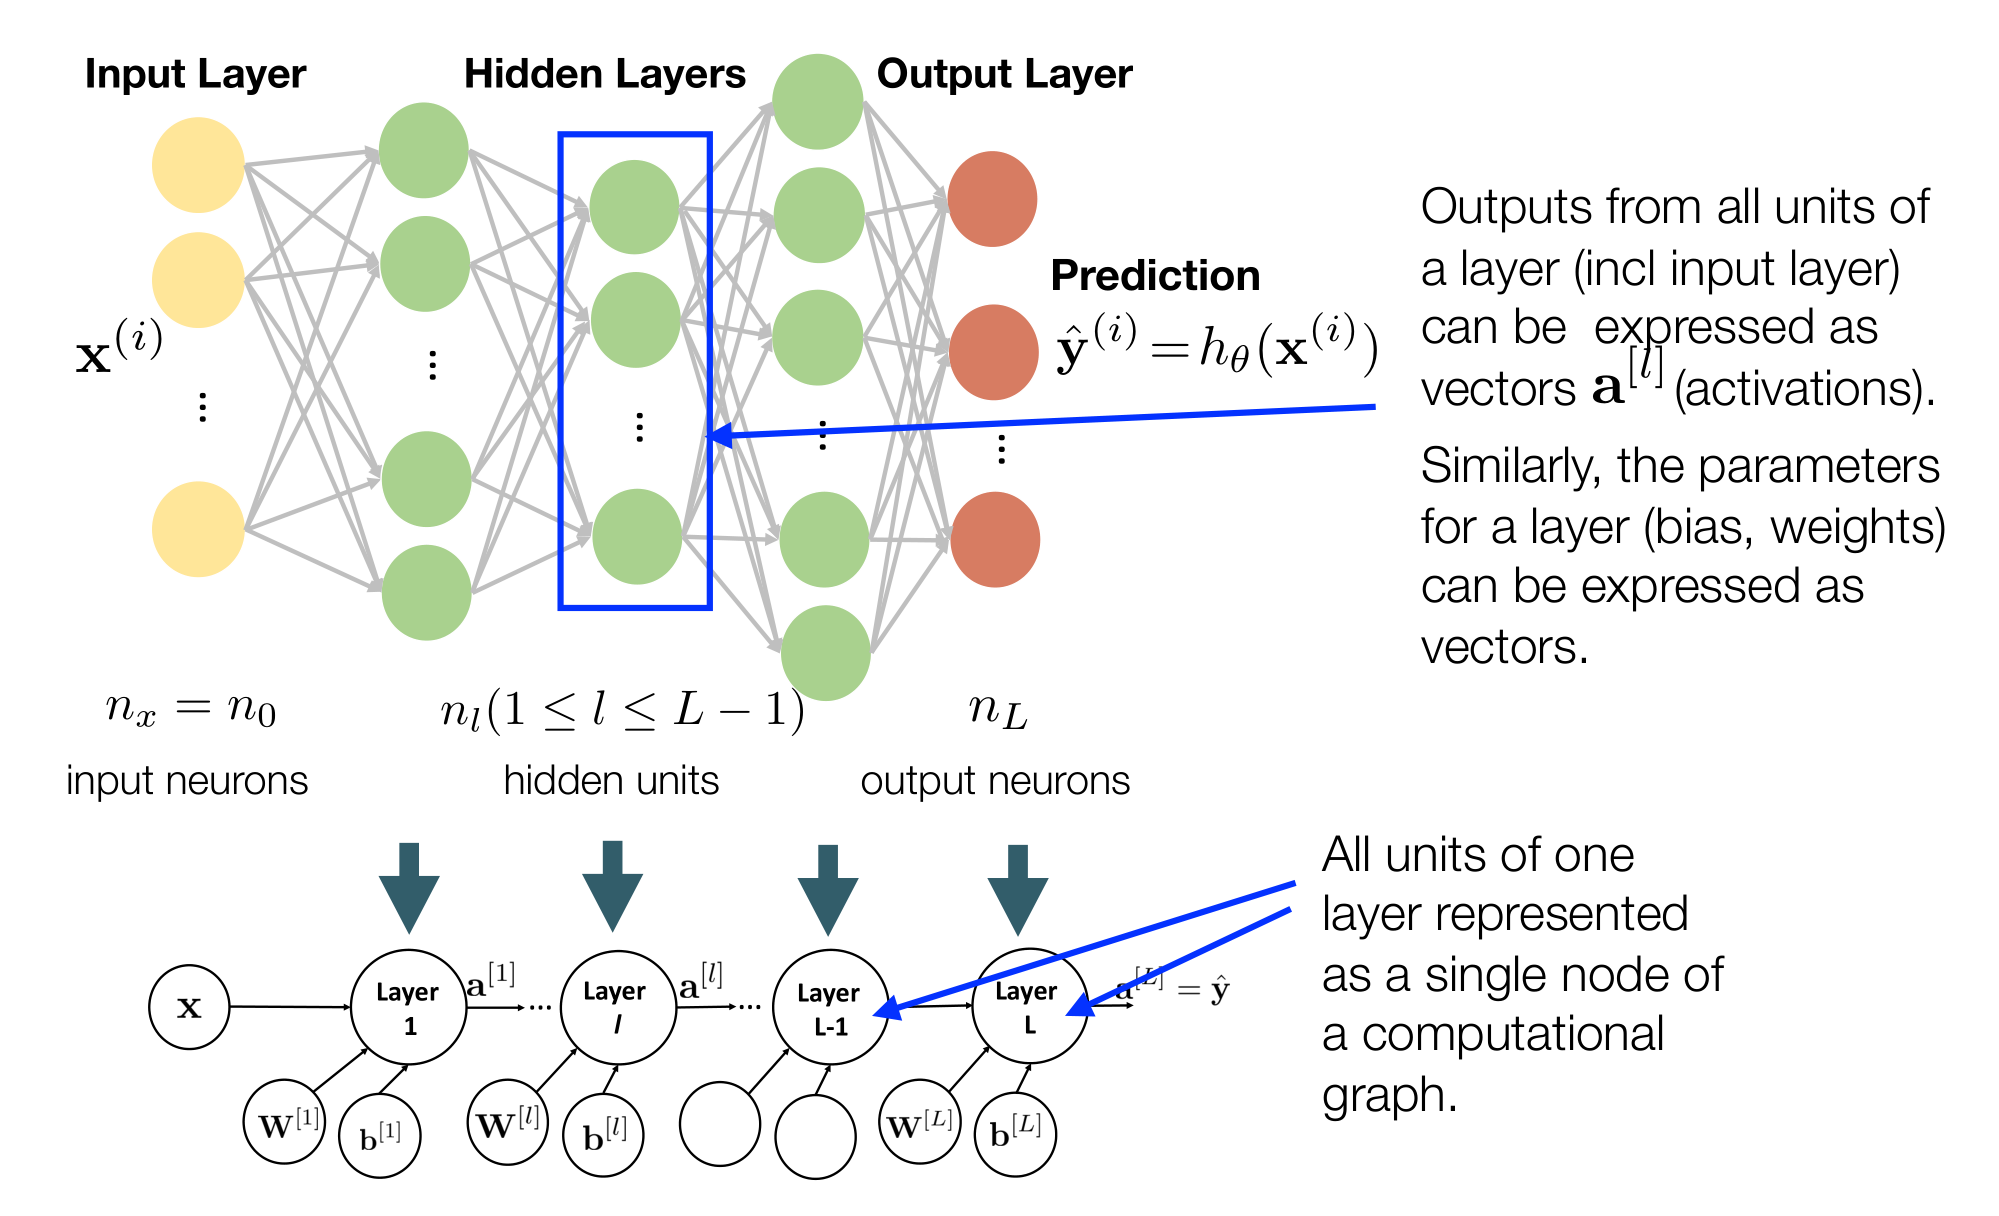
\includegraphics[width=0.9\linewidth]{mlp_layer_graph}
\end{figure}

\subsection{Notations for Layer in an MLP}

\noindent
\begin{figure}[H]
	\centering
	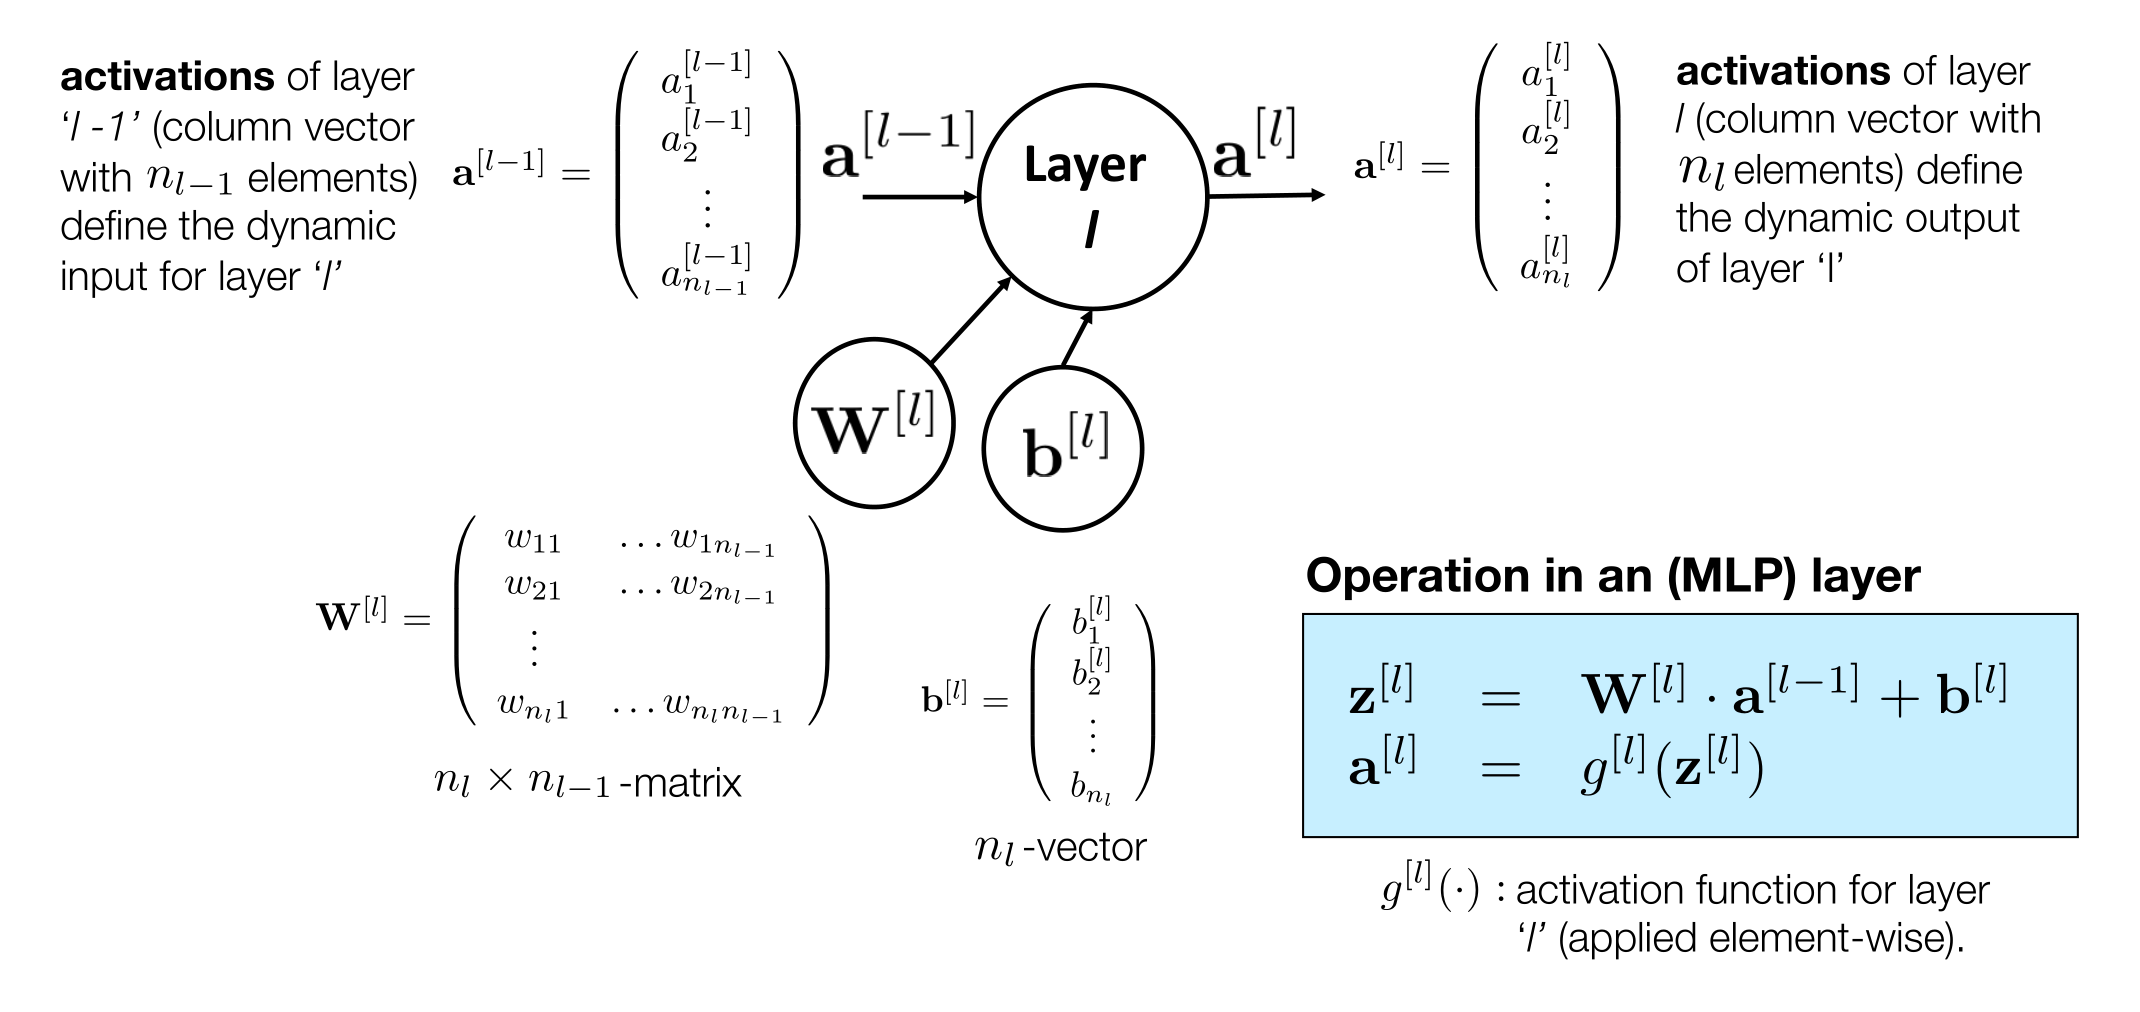
\includegraphics[width=0.9\linewidth]{mlp_layer_notations}
\end{figure}

Forward Propagation chains the calculations of activations in a MLP.

\begin{align*}
	z^{[1]} &= \textbf{W}^{[1]}\cdot\textbf{a}^{[0]} + \textbf{b}^{[1]}\\
	\textbf{a}^{[1]} &= g^{[1]}(\textbf{z}^{[1]})\\
	z^{[2]} &= \textbf{W}^{[2]}\cdot\textbf{a}^{[1]} + \textbf{b}^{[2]}\\
	\textbf{a}^{[2]} &= g^{[2]}(\textbf{z}^{[2]})\\
	\vdots\\
	z^{[L]} &= \textbf{W}^{[L]}\cdot\textbf{a}^{[L-1]} + \textbf{b}^{[L]}\\
	\textbf{a}^{[L]} &= g^{[L]}(\textbf{z}^{[L]})\\
	L(\widehat{\textbf{y}},\textbf{y}) &= \textbf{a}^{[L]}
\end{align*}

\subsection{Computing the Output of the MLP with Vectors}

Vectorise over the samples in a (mini-)batch. This will allow for efficient parallelisation on GPU. Put the input samples $\textbf{x}^{(i)}$ as columns in a $n_x\times m$ - matrix:
\begin{equation*}
	\textbf{X} = \textbf{A}^{[0]} = \begin{pmatrix}
	\vdots & \vdots & & \vdots\\
	\textbf{x}^{(1)} & \textbf{x}^{(2)} & \cdots & \textbf{x}^{(m)}\\
	\vdots & \vdots & & \vdots\\
	\end{pmatrix}
\end{equation*}

\noindent
The same for the activations and logits in the layer $l=1,...,L$ ($n_l\times m$ - matrices)

\begin{align*}
	\textbf{A}^{[l]} &= \begin{pmatrix}
		\vdots & \vdots & & \vdots\\
		\textbf{a}^{[l](1)} & \textbf{a}^{[l](2)} & \cdots & \textbf{a}^{[l](m)}\\
		\vdots & \vdots & & \vdots\\
	\end{pmatrix}\\
	\textbf{Z}^{[l]} &= \begin{pmatrix}
	\vdots & \vdots & & \vdots\\
	\textbf{z}^{[l](1)} & \textbf{z}^{[l](2)} & \cdots & \textbf{z}^{[l](m)}\\
	\vdots & \vdots & & \vdots\\
	\end{pmatrix}	
\end{align*}

\noindent
Then the equations for layer $l=1,...,L$ can then be written in a very compact manner
\begin{align*}
	\textbf{Z}^{[l]} &= \textbf{W}^{[l]}\cdot\textbf{A}^{[l-1]} + \textbf{b}^{[l]}\\
	\textbf{A}^{[l]} &= g^{[l]} (\textbf{Z}^{[l]})
\end{align*}

\subsection{Chain Rule of Calculus}
Rule to compute the derivative of a function with a nested structure, represented as a chain of function evaluations. According to the chain rule, the change is given by the product of the changes in the nested components. Thus a progressive calculation of inner derivatives can be done

\begin{align*}
	L(x) &= f(g(h(k(x))))\\
	\underbrace{dL}_{\text{change in target}} &= \frac{\partial f}{\partial g}\cdot\frac{\partial g}{\partial h}\cdot\frac{\partial h}{\partial k}\cdot\frac{\partial k}{\partial x}\cdot \underbrace{dx}_{\text{change in input variable}}\\
	&=f'(g(h(k(x)))) \times g'(h(k(x))) \times h'(k(x)) \times k'(x)
\end{align*}

\subsubsection{Example of the Chain Rule}
\begin{align*}
	f(x) &= \sqrt{1+x^2},\quad g(z) = \sqrt{z},\quad h(x) = 1+x^2\\
	f(x) &= g(h(x))\\
	\frac{df}{dx}(x) &= \underbrace{\frac{dg}{dz} (z=h(x))}_{\frac{dg}{dz}(z) = \frac{1}{2\sqrt{z}}} \cdot \underbrace{\frac{dh}{dx}(x)}_{\frac{dh}{dx}(x) = 2x}\\
	\frac{df}{dx}(x) &= \frac{dg}{dz}(z)\cdot \frac{dh}{dx} = \frac{1}{2\sqrt{z}} \cdot 2x \overset{z=h(x)}{=} \frac{1}{2\sqrt{1+x^2}} \cdot 2x = \frac{x}{\sqrt{1+x^2}}
\end{align*}

\subsection{Chain Rule in regards to the Computational Graph}
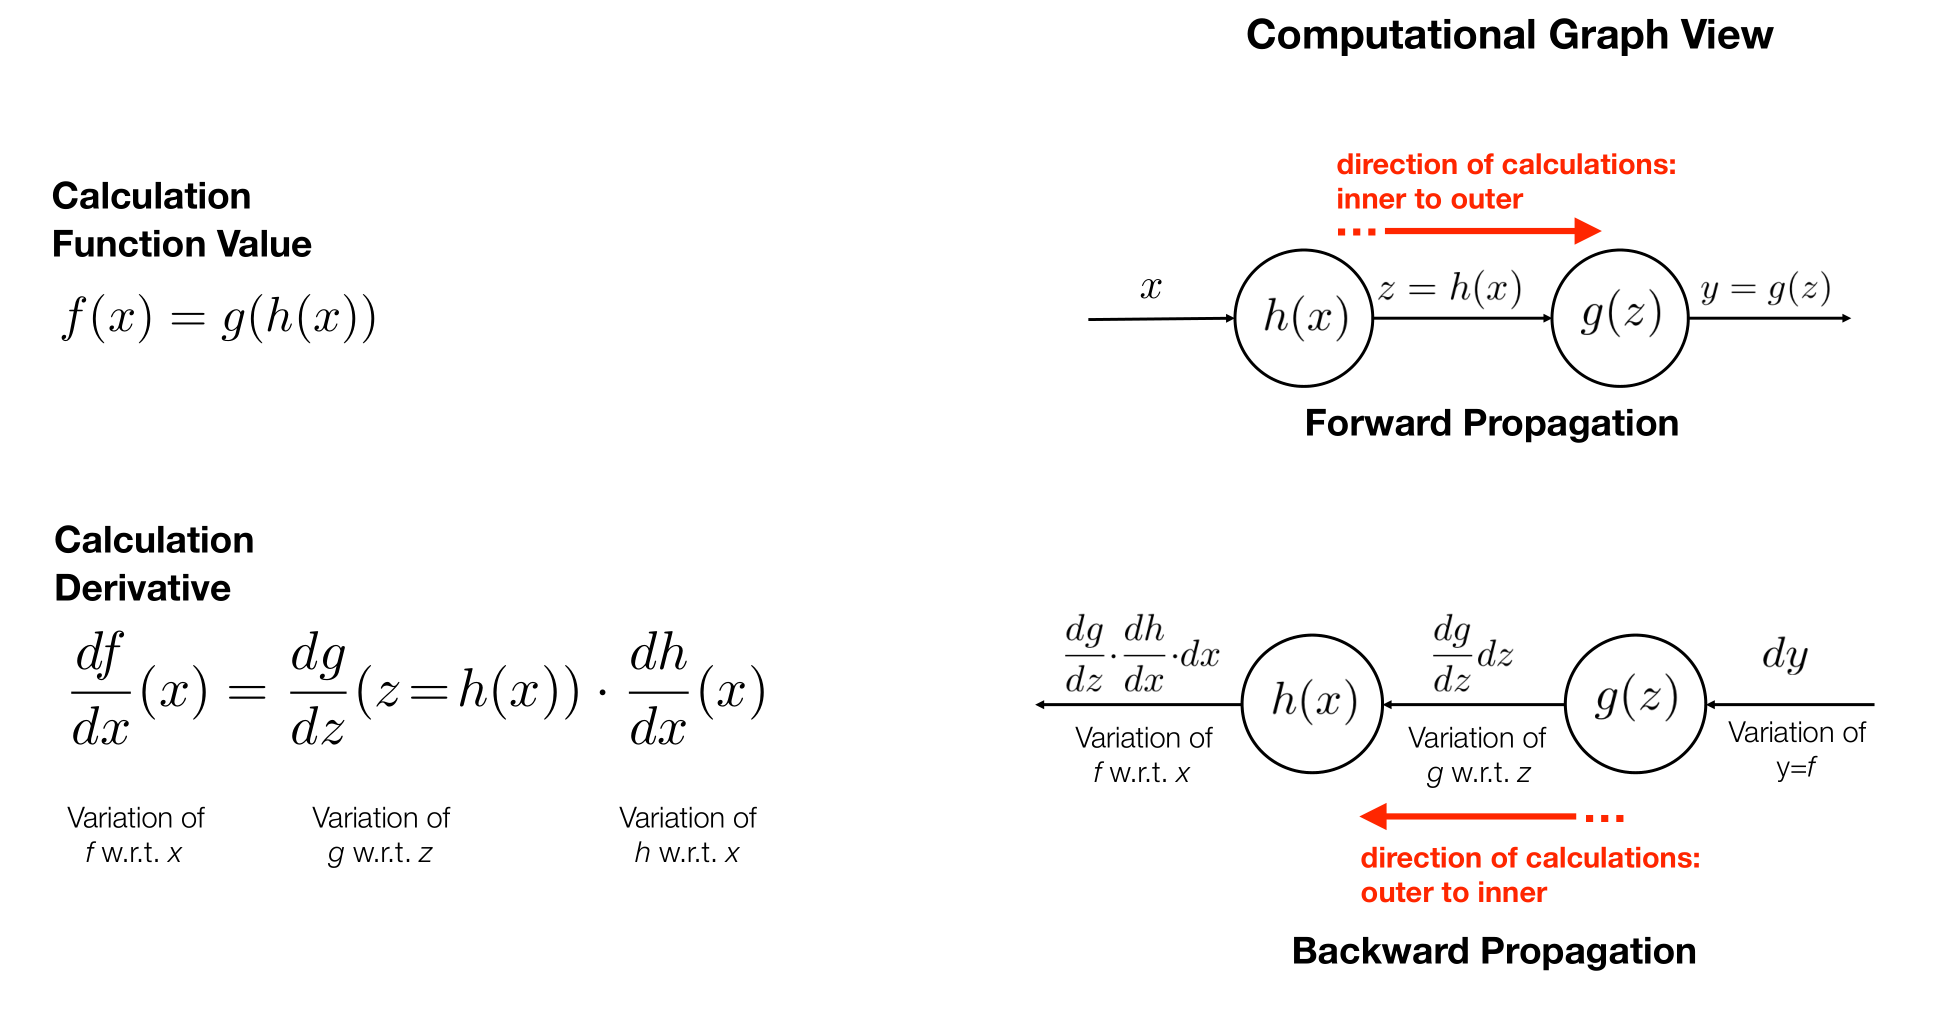
\includegraphics[width=0.8\linewidth]{chain_rule_computational_graph}

\subsection{Backpropagation Contribution per Node}
Steps to compute the change of a function represented by a computational graph with regard to the input variable (derivative):

\noindent
\begin{minipage}{0.6\linewidth}
	Start at the end of the computational graph and progressively walk back through the graph and initialise the result with 1.
	
	At each node, multiply the result obtained so far with the derivative of the node function with regard to the node input.
\end{minipage}
\begin{minipage}{0.4\linewidth}
	\centering
	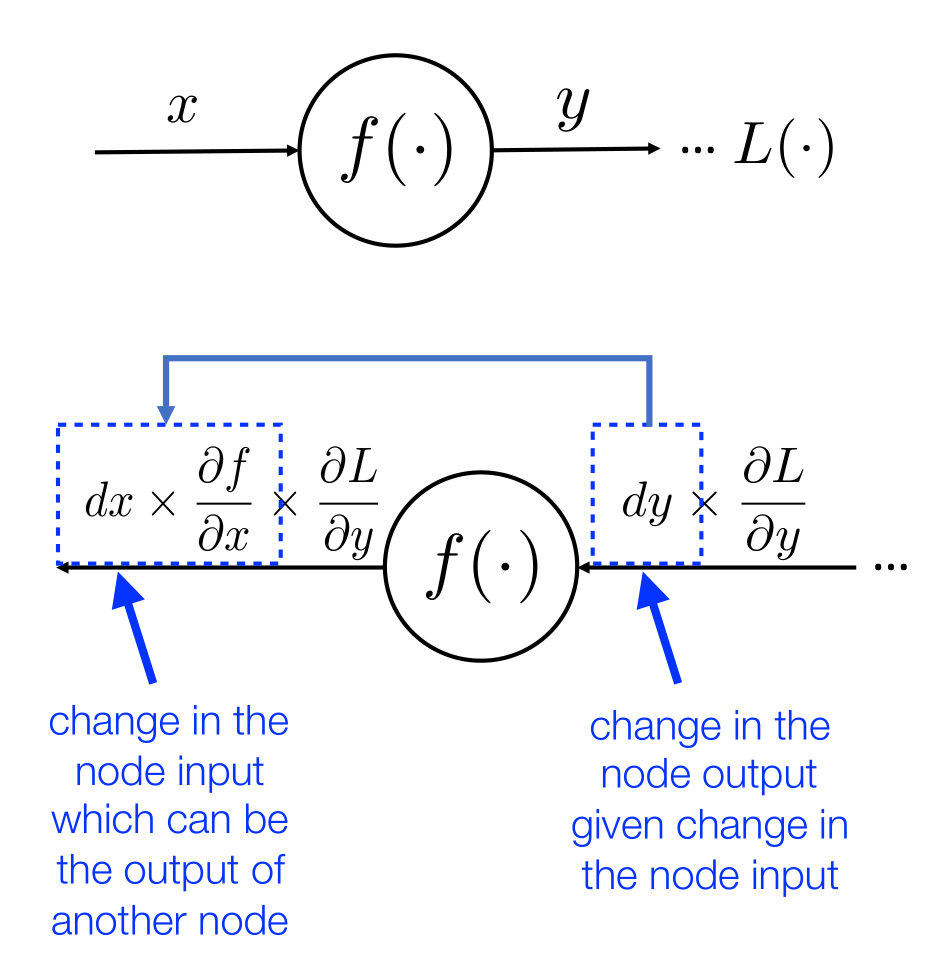
\includegraphics[width=\linewidth]{img/backprop_contrib_node}
\end{minipage}

\noindent
\begin{minipage}{0.6\linewidth}
	If the node has multivariate input, then compute the change in the output with regard to the change in each input variable (partial derivarive) separately. Then compute the change in the input variable by further traversing the graph structure in backwards direction.
\end{minipage}
\begin{minipage}{0.4\linewidth}
	\centering
	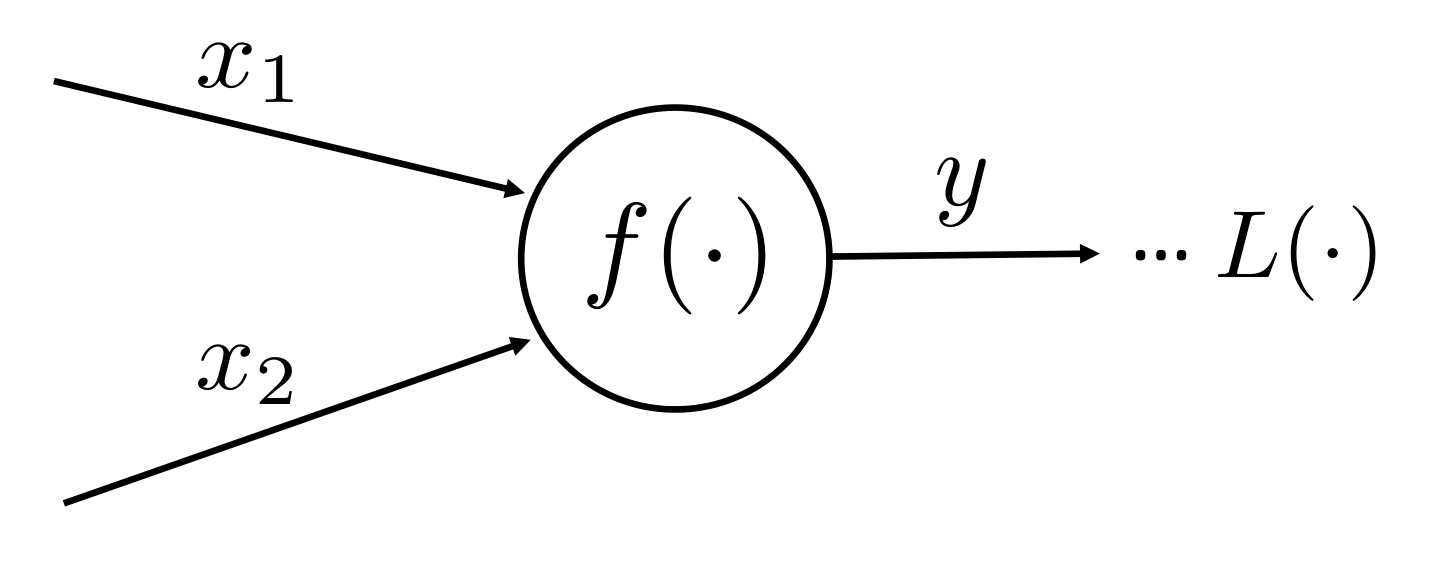
\includegraphics[width=\linewidth]{img/backprop_contrib_node_multivariate}
	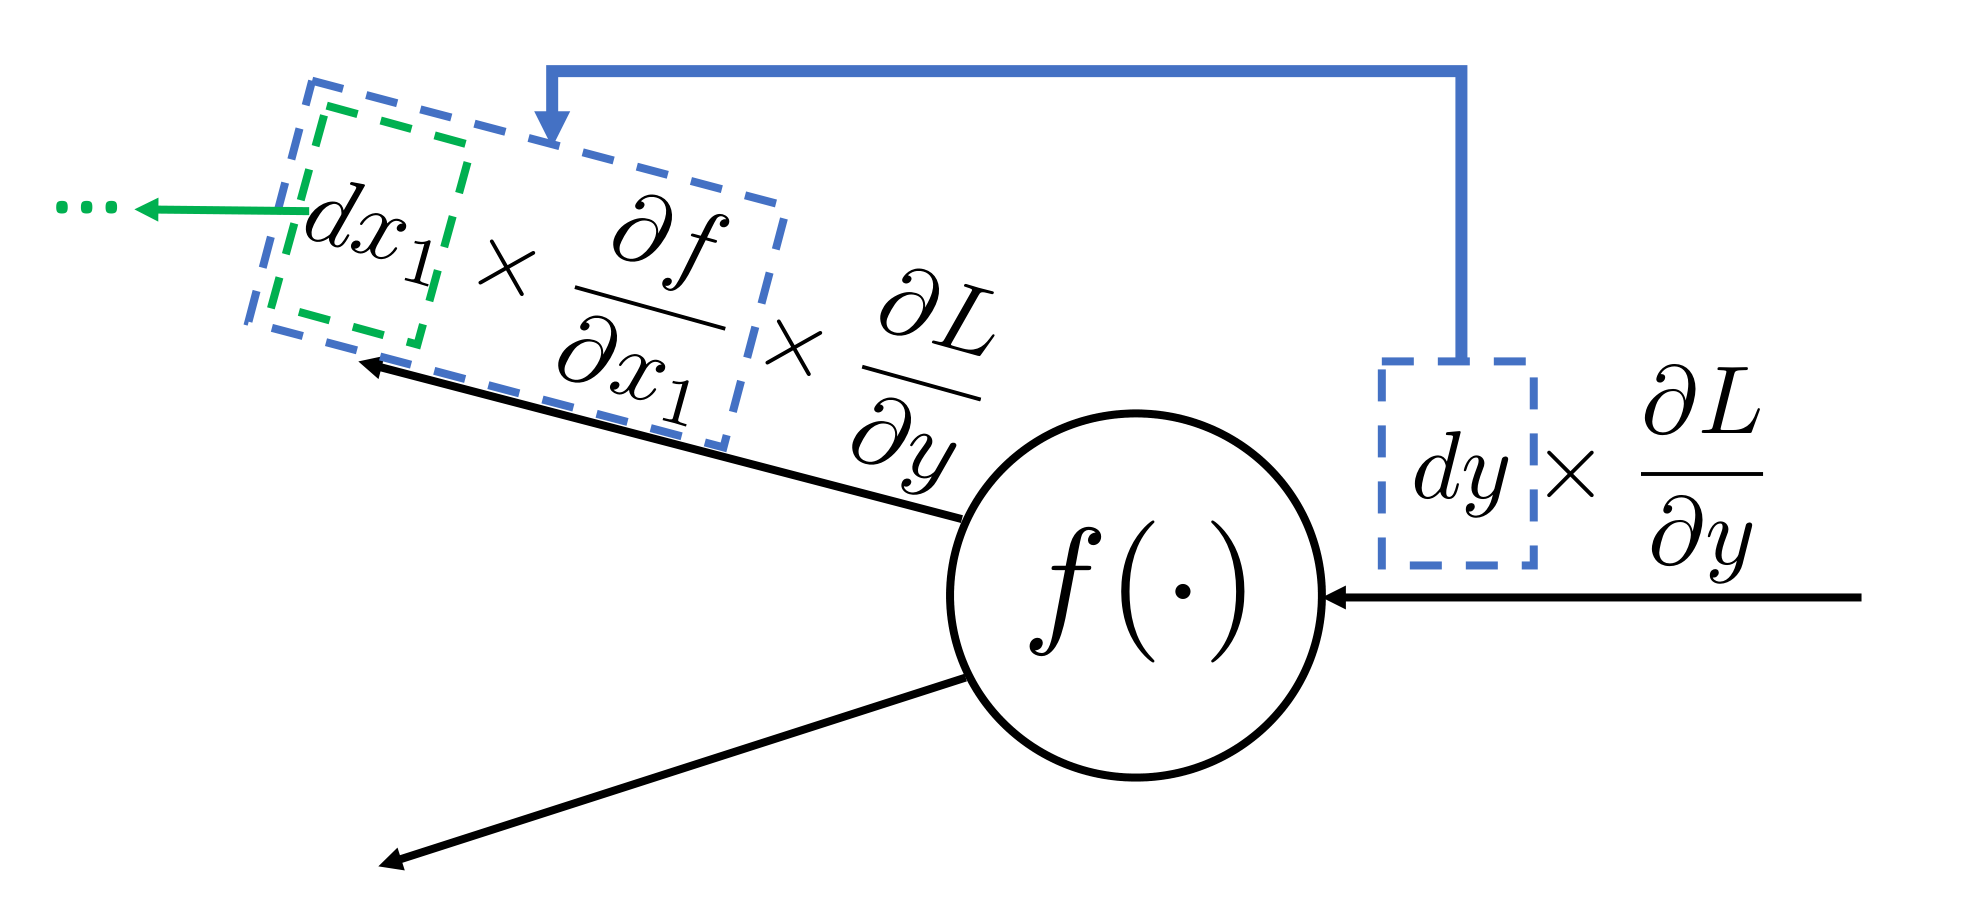
\includegraphics[width=\linewidth]{img/backprop_contrib_node_multivariate2}
\end{minipage}

\noindent
If several paths within the computational graph trace back to the same node (input or intermediary), the contributions from the different paths are summed.

\begin{center}
	\includegraphics[width=0.8\linewidth]{img/backprop_contrib_node_sum}
\end{center}

\subsection{Backpropagation Through a Single Layer}
\paragraph{Forward Propagation} Layer represented by a single node
\begin{center}
	\includegraphics[width=0.8\linewidth]{img/forward_propagation_single_layer}
\end{center}

\paragraph{Backward Propagation} Proper handling of tensor indices ignored
\begin{center}
	\includegraphics[width=0.8\linewidth]{img/forward_propagation_single_layer}
\end{center}

\begin{center}
	\includegraphics[width=0.8\linewidth]{img/backward_propagation_single_layer2}
\end{center}

\begin{equation*}
	\frac{\partial L}{\partial a_k^{[l-1]}} = \sum_{j}\frac{\partial L}{\partial z_j^{[l]}}\frac{\partial z_j^{[l]}}{\partial a_k^{[l]}} \qquad \frac{\partial L}{\partial W_{ki}^{[l]}} = \sum_{j}\frac{\partial L}{\partial z_j^{[l]}}\frac{\partial z_j^{[l]}}{\partial W_{ki}^{[l]}}\qquad\frac{\partial L}{\partial b_k^{[l]}} = \sum_{j}\frac{\partial L}{\partial z_j^{[l]}}\frac{\partial z_j^{[l]}}{\partial b_k^{[l]}}
\end{equation*}

\subsection{Derivatives for Chosen Layers}
\begin{figure}[H]
	\centering
	\includegraphics[width=0.8\linewidth, keepaspectratio]{normal_layer_derivatives}
	\caption{Derivatives for a normal layer (not softmax or cross-entropy)}
	\label{fig:normallayerderivatives}
\end{figure}

\begin{figure}[H]
	\centering
	\includegraphics[width=0.8\linewidth, keepaspectratio]{output_layer_derivatives}
	\caption{Derivatives for softmax and cross-entropy layers}
	\label{fig:outputlayerderivatives}
\end{figure}

\subsection{Vectorised Formulation of Forward and Backward Propagation}

\paragraph{Forward Propagation}
\begin{align*}
	\textbf{Z}^{[L]} &= \textbf{W}^{[l]}\cdot\textbf{A}^{[l-1]}+\textbf{b}^{[l]}\\
	\textbf{A}^{[l]} &= g^{[l]} \textbf{Z}^{[l]}
\end{align*}

\paragraph{Backward Propagation}
\begin{align*}
	\frac{\partial L}{\partial \textbf{A}^{[l-1]}} &= \frac{\partial L}{\partial \textbf{Z}^{[l]}}\frac{\textbf{Z}^{[l]}}{\partial \textbf{A}^{[l-1]}} = (\textbf{W}^{[l]})^T\cdot\frac{\partial L}{\partial \textbf{Z}^{[l]}}\\
	\frac{\partial L}{\partial \textbf{W}^{[l]}} &= \frac{\partial L}{\partial \textbf{Z}^{[l]}} \cdot \frac{\partial \textbf{Z}^{[l]}}{\partial \textbf{W}^{[l]}} = \frac{\partial L}{\partial \textbf{Z}^{[l]}}(\textbf{A}^{[l-1]})^T\\
	\frac{\partial L}{\partial \textbf{b}^{[l]}} &= \frac{\partial L}{\partial \textbf{Z}^{[l]}} \cdot \frac{\partial \textbf{Z}^{[l]}}{\partial \textbf{b}^{[l]}} = \text{sum}\left(\frac{\partial L}{\partial \textbf{Z}^{[l]}}, \text{axis}=1\right)\\
	\frac{\partial L}{\partial \textbf{Z}^{[l]}} &= \frac{\partial L}{\partial \textbf{A}^{[l]}}\cdot\frac{\partial \textbf{A}^{[l]}}{\partial \textbf{Z}^{[l]}} = \frac{\partial L}{\partial \textbf{A}^{[l]}} \ast g^{[l]}\textquotesingle(\textbf{Z}^{[l]})
\end{align*}

$\ast$: element-wise multiplication

\subsubsection{A Simple Numerical Example}

\includegraphics[width=\linewidth,keepaspectratio]{forward_backward_propagation_numerical_example}

\subsection{Advantages of Computational Graphs}
\begin{enumerate}
	\item Intuitive interpretation of gradient backpropagation
	\item We can easily define new nodes using the forward/backward pattern
	\item Node composition or factorisation: any complex learning architecture can be composed from atomic nodes. No need to compute complex global gradient
	\item The loss functions can actually be seen as extra nodes in the graph
\end{enumerate}

Meta-nodes like the Sigmoid can be composed of multiple atomic nodes, or equivalently, a sub-graph composed of nodes can be re-implemented in a single node if an analytic form of the gradients can be computed.

\section{Keras}
Keras is a high-level open-source neural networks API, written in Python and capable of running on top of \textbf{TensorFlow}, \textbf{CNTK}, or \textbf{Theano}. It was developed with a focus on enabling fast experimentation.

A \textbf{model} is the way Keras organises the layers of neurons, it is differentiated between the sequential and the functional model. The sequential model corresponds to a regular stack of feed-forward layers. The functional API allows to define \textbf{graphs} of layers and is used to construct non-sequential architectures. It is typically used to allow for independent networks to diverge or merge.

Dense layers represent fully connected layers of neurons in Keras, they are added as follows:
\begin{minted}{python}
model.add(tf.keras.layers.Dense(H, input_shape=(D,), activation='relu'))
# The input shape is inferred from the output shape of the preceding layer
model.add(tf.keras.layers.Dense(n_classes, activation='sigmoid'))
\end{minted}

\subsubsection{Complex Example}
\begin{minted}[linenos, breaklines]{python}
import tensorflow as tf

model = tf.keras.models.Sequential()
model.add(tf.keras.layers.Dense(10, input_shape=(D,), use_bias=False, activation='relu'))

# Print the model parameters
model.summary()

# Define custom Optimiser
sgd = tf.keras.optimizers.SGD(learning_rate=0.5)

# Prepare the model for training with MSE cost function and SGD Optimiser, train on accuracy of the model
model.compile(optimizer=sgd, loss='mse', metrics=['accuracy'])

# Train the model
history1 = model.fit(x_train, y_train, batch_size=N, epochs=40)
# Show test fit
model.evaluate(x_test, y_test, verbose=2)
\end{minted}

\begin{figure}[tbh]
	\centering
	\includegraphics[width=0.5\linewidth,keepaspectratio]{keras_model_example}
	\caption{The model in the example}
	\label{fig:kerasmodelexample}
\end{figure}

\subsection{Functional API of Keras}
The \textbf{sequential} model of Keras corresponds to a regular stack of layers while the \textbf{functional} API is used for non sequential architectures. The functional API allows for multiple paths in the computational graph through layer sharing, multiple inputs, and multiple outputs.

Unlike the Sequential model, one must create and define a stand-alone Input layer that specifies the shape of input data. The input layer takes a shape argument that is a tuple that indicates the dimensionality of the input data. When input data is one-dimensional, such as for a MLP, the shape must explicitly leave room for the shape of the mini-batch size. Therefore, the shape tuple is always defined with a hanging last dimension when the input is one-dimensional. 

The layers in the model are connected pairwise. This is done by specifying where the input comes from when defining each new layer. A callable syntax is used, such that once the layer is created, the layer from which the input is taken is specified through a call.

A Model is declared with its inputs and its outputs that are both tensors defining the inputs and outputs of the computational graph.

\begin{minted}[breaklines]{python}
H = 300 # number of neurons
D = X_train.shape[1] # dimension of input - 784 for MNIST

#Keras functional API, note the dangling last dimension in the input shape
visible = Input(shape=(D,)) # func api, input is declared
# visible layer is passed through the callable syntax
hidden1 = Dense(H, activation='relu')(visible)
output = Dense(n_classes, activation='softmax')(hidden1)
model2 = Model(inputs=visible, outputs=output)
model2.summary()
\end{minted}

\subsubsection{Python \mintinline{python}{callable} syntax}
Objects are callable when the class definition includes a \mintinline{python}{__call__} method. It allows to call the object as we would call a method with the syntax \mintinline{python}{obj()}.

\subsubsection{CNN Multiple Paths Example}

\begin{minipage}{0.6\linewidth}
	\begin{minted}[breaklines,fontsize=\tiny]{python}
# Shared Input Layer
from tensorflow.keras.utils import plot_model
from tensorflow.keras.models import Model
from tensorflow.keras.layers import Input, Dense, Dropout
from tensorflow.keras.layers import Flatten, Conv2D
from tensorflow.keras.layers import MaxPooling2D, concatenate

# input layer
visible = Input(shape=(28,28,1))
# first feature extractor
conv1 = Conv2D(32, kernel_size=3, activation='relu')(visible)
drop1 = Dropout(0.2)(conv1)
pool1 = MaxPooling2D(pool_size=(2, 2))(drop1)
flat1 = Flatten()(pool1)
# second feature extractor
conv2 = Conv2D(32, kernel_size=6, activation='relu')(visible)
drop2 = Dropout(0.2)(conv2)
pool2 = MaxPooling2D(pool_size=(2, 2))(drop2)
flat2 = Flatten()(pool2)
# merge feature extractors
merge = concatenate([flat1, flat2])
# interpretation layer
hidden1 = Dense(100, activation='relu')(merge)
# prediction output
output = Dense(10, activation='softmax')(hidden1)
model4 = Model(inputs=visible, outputs=output)
# summarize layers
print(model4.summary())
# plot graph
plot_model(model4, to_file='shared_input_layer.png')
	\end{minted}
\end{minipage}
\begin{minipage}{0.4\linewidth}
	\begin{center}
		\includegraphics[width=\linewidth]{img/keras_funcitonal_api_multiple_path_cnn}
	\end{center}
\end{minipage}

\subsubsection{Multiple Inputs}
Such graphs are useful to merge different modalities, such as multiple images of the same object, stereo speech recordings, or different parameters of an acquisition device.

\subsubsection{Callbacks}
Callback are functions to be applied at given stages of the training procedure. Callbacks can be used to get a view on internal states and statistics of the model during training.  Some are automatically applied in the fit() method such as BaseLogger and History.
\begin{minted}[breaklines, fontsize=\small]{python}
B = 128
E = 10
checkpoint = ModelCheckpoint('model-{epoch:03d}.h5', verbose=1, monitor='val_accuracy',save_best_only=True, mode='auto')
model5.compile(loss='categorical_crossentropy', optimizer='rmsprop', metrics=['accuracy'])
log = model5.fit(X_train, Y_train, batch_size=B, epochs=E, verbose=1, validation_data=(X_test, Y_test), callbacks=[checkpoint])
\end{minted}

\subsubsection{Best Practices}
\begin{itemize}
	\item \textbf{Use Consistent Variable Names}\quad Use same variable name for input (visible) and output layers (output), hidden layers (hidden1, hidden2)
	\item \textbf{Review Layer Summary}\quad Always print the model summary and review the layer outputs to ensure that the model was connected together as you expected
	\item \textbf{Review Graph Plots}\quad Create a plot of the model graph and review it to ensure that everything was put together as you intended
	\item \textbf{Name the layers}\quad Assign names to layers that are used when reviewing summaries and plots of the model graph
	\item \textbf{Use Callbacks}\quad Use callbacks to save the best models from epochs to epochs as a safety against interrupt and overfitting
\end{itemize}

\section{Regularisation and Faster Optimisers}

\subsection{Vanishing and Exploding Gradients}
There were some difficulties in training deep neural nets in 2007 with the given techniques that were available. These difficulties were mitigated through various improvements, important contributions were made from Glorot, Bengio, Ioffe, Szegedy and others.

These aim at avoiding the saturation regions of the activation functions at early stages of the training by stabilising the variance when propagating forward and backward, and choosing more suitable activation functions that differ from the sigmoid.

In the so-called saturation regions the gradients are close to zero and become even smaller when they are back-propagated. This means that learning comes to a standstill. The suggested solution was to use suitably initialised parameters with the "Glorot" or "Xavier" initialisation and a non-sigmoidal activation function.

\subsubsection{Reason for Vanishing Gradients}

When backpropagating through the neural network the chain rule of calculus is used, this means we have a product term with derivatives of the neuron's activation function.
\begin{align*}
	\frac{\partial L}{\partial w^{[l]}} &= a^{[l-1]}\cdot g'\left(z^{[l]}\right)\cdot \left(\prod_{k=l+1}^{L}w^{[k]}g'(z^{[k]})\right)\cdot\frac{\partial L}{\partial a^{[l]}}\\
	\frac{\partial L}{\partial b^{[l]}} &= g'\left(z^{[l]}\right)\cdot \left(\prod_{k=l+1}^{L}w^{[k]}g'(z^{[k]})\right)\cdot\frac{\partial L}{\partial a^{[l]}}
\end{align*}

This product term is responsible for gradients to shrink to zero or becoming too large.
\begin{equation*}
	\sigma'(z) = \sigma(z)(1-\sigma(z))
\end{equation*}
This product term gets small or very small for large values of z (label correct or completely wrong). The problem can be alleviated through
\begin{itemize}
	\item \textbf{Parameter Initialisation} Properly initialise the weights so that the logits z do not grow too large in magnitude
	\item \textbf{Batch Normalisation, Gradient Clipping} Make sure that the weights do not grow too large in magnitude during training
	\item \textbf{Suitable Activation Functions} Use activation functions that cannot saturate
\end{itemize}

\subsection{Xavier/He Initialisation}
\begin{itemize}
	\item \textbf{Randomly initialise weights} to break symmetries at start of the learning
	\item \textbf{Initialise weights at proper scale} to keep the variance stable across layers, ideally in forward and backward propagation. Properly scaling the width of the distribution depends on the random distribution used to generate the weights and activation function (refer to figure \ref{fig:activationfunctiondistributions}).
\end{itemize}

\begin{figure}[tbh]
	\centering
	\includegraphics[width=0.6\linewidth, keepaspectratio]{activation_function_distributions}
	\caption{Different distribution for activation functions}
	\label{fig:activationfunctiondistributions}
\end{figure}

\subsubsection{Parameter Initialisation in Keras}
\begin{figure}[H]
	\centering
	\includegraphics[width=0.7\linewidth]{parameter_initialisation_in_keras}
	\caption{Example initialisation of parameters in Keras}
	\label{fig:parameterinitialisationinkeras}
\end{figure}

\subsection{Batch Normalisation}
Idea introduced by Ioffe and Szegedy to normalise the input to each layer per mini-batch just before applying the activation function, estimate mean and standard deviation used for the normalisation from the current mini-batch. Afterwards, let the model learn the optimal scale and mean of the inputs for each layer.

It proves very effective for improving the stability of the training, and significantly reduces the problem of coordinating updates across many layers. It also limits the amount to which parameter updates in earlier layers can affect the distribution of values the later layers see, and can be applied to any input or hidden layer in the network.

Ioffe and Szegedy  recommend to apply batch normalisation to the inputs to the activation function, that is the logits $z_k^{[l]}$.
\paragraph{Normalisation per Mini-Batch}
\begin{equation*}
	\left(Z_{\text{norm}}^{\{r\},[l]}\right)_{k,i} = \frac{Z_{k,i}^{\{r\},[l]}-\mu_{k}^{\{r\},[l]}}{\sigma_{k}^{\{r\},[l]} + \epsilon}
\end{equation*}
\paragraph{Scaling and Shifting}
\begin{equation*}
\left(\widehat{Z}_{\text{norm}}^{\{r\},[l]}\right)_{k,i} = \gamma_k^{[l]}\left(Z_{\text{norm}}^{\{r\},[l]}\right)_{k,i} + \beta_k^{[l]}
\end{equation*}
$\gamma_k^{[l]}$ and $\beta_k^{[l]}$ are parameters to be learned and optimised.

\subsection{Non-Saturating Activation Functions}
Avoid S-shaped activation functions that flatten out at larger z-magnitudes, such as ReLU, LeakyReLU or ELU

\subsection{Gradient Clipping}
Counter \emph{exploding gradients} by simply clipping gradients in length during back-propagation. Intuition provided by I. Goodfellow: Deep networks often have extremely steep regions resembling cliffs - as a result of the composite structure of the operations where weights get multiplied. At the cliffs, the gradient can be become very large.

\begin{figure}[H]
	\centering
	\includegraphics[width=0.6\linewidth, keepaspectratio]{exploding_gradients_intuition}
	\caption{The first update steps lead towards the minimum, but overshoots and gets into the "cliff region" where the gradients explode away from the minimum (I. Goodfellow "Deep Learning")}
	\label{fig:explodinggradientsintuition}
\end{figure}

\section{Advanced Optimisation Methods}
\subsection{Overview on Optimisers}
\paragraph{Stochastic Gradient Descent} Vanilla GD (BGD, MBGD, SGD)
\begin{minted}{python}
tf.optimizers.SGD(learning_rate=0.1)
\end{minted}
\paragraph{Momentum, Nesterov} Allows to surpass flat regions or saddle points — like a ball that keeps on rolling down if it has an initial speed when entering flat regions
\begin{minted}{python}
tf.optimizers.SGD(learning_rate=0.01, momentum=0.9, nesterov=True)
\end{minted}
\paragraph{RMS Prop} Adaptively adjusts the learning rate to incorporate differences in the steepness along different directions in parameter space
\begin{minted}{python}
tf.optimizers.RMSProp(learning_rate=0.01)
\end{minted}
\paragraph{Adam} Combination of Momentum / Nesterov and RMSprop, state of the art right now, but active field of research
\begin{minted}{python}
tf.optimizers.Adam(learning_rate=0.001*lr)
\end{minted}

\subsubsection{Momentum, Nesterov}
It's a modified schme for computing the gradient, with a notion of a momentum encoded within. Algorithm: Compute an exponentially decaying moving average of past gradients and move in the direction of the moving average.
\begin{align*}
	\textbf{m} &\leftarrow \beta_1 \textbf{m} +\alpha\nabla J(\theta)\\
	\theta &\leftarrow \theta - \textbf{m}
\end{align*}
$\beta_1$ is the 'momentum' hyper-parameter which controls the decay and the friction (large friction and fast decay with small values of $\beta_1$ and vice versa, a good default is $\beta_1 = 0.9$).

With the Nesterov scheme the algorithm gets modified, which is considered to be efficient
\begin{align*}
	\textbf{m} &\leftarrow \beta_1 \textbf{m} +\alpha\nabla J(\theta + \beta_1\textbf{m})\\
	\theta &\leftarrow \theta - \textbf{m}
\end{align*}

\subsubsection{Adam Optimisation}
Combines Momentum and RMS Prop and is currently considered as the de facto standard.
\begin{align*}
	\textbf{m} &\leftarrow \beta_1 \textbf{m} + (1-\beta_1)\nabla J(\theta)\\
	\textbf{s} &\leftarrow \beta_2 \textbf{s} + (1-\beta_2)\nabla J(\theta)\odot\nabla J(\theta)\\
	\widehat{\textbf{m}} &= \frac{\textbf{m}}{1-\beta_1}\\
	\widehat{\textbf{s}} &= \frac{\textbf{s}}{1-\beta_2}\\
	\theta &\leftarrow \theta - \alpha\frac{\widehat{\textbf{m}}}{\sqrt{\widehat{\textbf{s}}+\epsilon}}\odot\nabla J(\theta)
\end{align*}
$\odot$: Symmetric Tensor Product, Element-wise operations are adopted for the squared gradient, the division and square-root in the update step. Initialise $\textbf{m}$ and $\textbf{s}$ to 0. In order to avoid that at the beginning these terms are systematically smaller in magnitude, the steps 3\&4 are applied.

\begin{tabularx}{\linewidth}{X c c}
	Hyper-Parameter & Symbol & Default Value\\
	Learning Rate & $\alpha$ & 0.9\\
	Momentum & $\beta_1$ & 0.9\\
	RMS Decay & $\beta_2$ & 0.999\\
	Numerical Stabilisation & $\epsilon$ & $10^{-8}$
\end{tabularx}

\subsubsection{Learning Schedule}
Instead of adapting the learning rate in accordance with information collected during the optimisation process along the trajectory in parameter space, the learning rate may be manually adjusted in the different phases of learning (~epochs or update steps). Typically, a higher learning rate is used at the start and then reduced
\begin{center}
	\includegraphics[width=0.8\linewidth,keepaspectratio]{learning_schedule_schemes}
\end{center}

\subsection{Regularisation}
Regularisation is a mean to avoid overfitting. I. Goodfellow:

"Regularisation is any modification to a learning algorithm that is intended to reduce its generalisation error but not its training error."


\paragraph{Regularisation Methods}
\begin{itemize}
	\item \textbf{Weight Penalty} Constraints on parameters (length of parameter vector, number of parameters) to give preference to simple models
	\item \textbf{Dropout} Randomly drop (neutralise) neurons during training steps to make the solution less dependent on individual neurons
	\item \textbf{Early Stopping} Stop training at the minimum of the cost function on the validation set
	\item \textbf{Data Augmentation} Generate more training data with additional characteristics (symmetries) the solution should have
\end{itemize}

\subsubsection{Weight Penalty}
The loss function is modified to give preference to smaller or fewer weights.

\begin{equation*}
	J = J_{\text{data}} + J_{\text{reg}}
\end{equation*}
$J_{\text{data}}$: \textbf{Performance term}\quad how far differs the prediction on the data from the ground truth, $J_{\text{reg}}$: \textbf{Regularisation term}\quad limit the weights from becoming too large

\begin{equation*}
	\textbf{J} = \textbf{J}_0 + \lambda\cdot\Omega(\textbf{W})\qquad(\lambda\geq0)
\end{equation*}
\noindent
$\textbf{J}_0$: Original Loss Function, $\lambda$: Regularisation Parameter, $\Omega(\textbf{W})$: Penalty term that favours models with smaller and fewer weights.

Two forms of penalties are popular
\begin{tabularx}{\linewidth}{X l}
	$L_1$-Regularisation & $ \Omega(\textbf{W}) = \norm{\textbf{W}}_1 = \sum_{l,k,j}\norm{W_{kj}^{[l]}} $\\
	$L_2$-Regularisation & $ \Omega(\textbf{W}) = \norm{\textbf{W}}_2^2 = \sum_{l,k,j}\norm{W_{kj}^{[l]}}^2 $\\
\end{tabularx}

For optimisation with gradient descent, the derivatives of the loss are modified by the penalty term in a direction to make the loss and the penalty term smaller.

\begin{figure}[tbh]
	\centering
	\includegraphics[width=0.6\linewidth,keepaspectratio]{img/L1_L2_regularisation}
	\caption{Illustration of L1 and L2 regularisation}
	\label{fig:l1l2regularisation}
\end{figure}

\subsubsection{Dropout}
Most popular regularisation technique for deep neural networks, and highly succesfull: Even state-of-the-art neural networks get a 1-2\% accuracy increase simply by adding dropout.
\begin{itemize}
	\item At each training step, each neuron (including input neurons, excluding output neurons) has a probability $p$ (“dropout rate”) of being ignored during this step and having its activations masked
	\item Dropout rate typically set to 50\% for hidden, and 20\% for input units
	\item For testing or in production, neurons don’t get dropped, but weights or outputs are corrected (since weights are trained including the dropout rate)
\end{itemize}

The implications of using Dropout are that simpler models with less units are considered during training, models learn to be less dependent on single units and units cannot co-adapt with their neighbouring units, they have to be as useful as possible on their own. As a result a more robust network is obtained that generalises better.

\begin{itemize}
	\item Computationally very cheap\quad Drawing a random binary number for each unit, O(n) additional memory to store these numbers, no additional cost at test time or in production
	\item Very versatile\quad Is not limited to certain architectures or models, and can be combined with other regularisation techniques
	\item Reduced representational capacity\quad As a regularisation technique, dropout reduces the effective capacity of a model. For very large datasets, regularisation implies little reduction in generalisation error, so the computational cost of using dropout and larger models may outweigh the benefit of regularisation
\end{itemize}

\subsubsection{Early Stopping}
Stop training when validation error begins to increase while training error still decreases.

\begin{itemize}
	\item Run optimisation algorithm to train the model and simultaneously compute validation set error
	\item Store a copy of the model parameters as long as the validation set error improves
	\item Iterate until validation set error stops improving
	\item Return the parameters where the smallest validation set error is observed
\end{itemize}

Training time (number of training steps/epochs) is considered as hyper-parameter. Early Stopping controls the \emph{effective capacity} of the model by determining the number of steps it can take to fit the training set, thus restricting the volume in parameter space that can be searched. It's furthermore an efficient, non-intrusive search for this hyper-parameter and is easy to combine with other regularisation techniques.

\section{Convolutional Neural Networks}
The general idea behind CNNs was to define new type of layers and connections that will bring preservation of the spatial structure, hierarchical feature detection, to utilise the fact that objects in images are composed of features that are themselves composed of other features, and to have a robustness to object variabilities such as viewpoint, occlusion and more.

The challenges for image recognition is, amongst others, the intra-class variabilities the model is expected to handle.

\subsection{2D Signal Convolutional Layer}
The idea is to preserve the spatial structure in the original data with specialised layers coming from image processing, called filters or kernels.

\begin{center}
	\includegraphics[width=0.9\linewidth]{img/convolutional_layer_kernel}
\end{center}

The second idea is to \textbf{convolve the filter with the image}, that is to "slide" over the image spatially, computing dot products of the weights of the filter with the window of pixels where the filter is located. The sub-area of an input that influences a component of the output is sometimes called the \textbf{receptive field} of the latter. This produces a \textbf{activation map} that is the result of the convolution of the filter. This sliding of the filter gives us \textbf{translation invariance} regarding to what the filter is sensitive for. Several individual filters can produce several activation maps.

\begin{center}
	\includegraphics[width=0.8\linewidth]{img/convolutional_layer_kernels_stacked}
\end{center}

\subsection{1D Signal Convolutional Layer}

Given $x = (x_1,...,x_W)$ and a convolution kernel of width $u=(u_1,...,u_w)$, the convolution $x\circledast u$ is a vector of size $W-w+1$, with
\begin{equation*}
	(x\circledast u)_i = \sum_{j=1}^{w}x_{i-1+j}\cdot u_j = (x_i, ..., x_{i+w-1})\cdot u
\end{equation*}

Example:
\begin{equation*}
	(1,2,3,4)\circledast(3,2) = (3+4,6+6,9+8) = (7,12,17)
\end{equation*}

Such filter can be differential operators 
\begin{center}
	\includegraphics[width=0.8\linewidth]{img/convolutional_layer_kernels_differential}
\end{center}
or match simple shapes
\begin{center}
	\includegraphics[width=0.8\linewidth]{img/convolutional_layer_kernels_template}
\end{center}

Input images usually have three channels for colour, thus the filters should have the same depth. The activation map have a depth equal to the number of fiters.
\begin{center}
	\includegraphics[width=0.8\linewidth]{img/convolutional_layer_kernels_depth}
\end{center}

\subsection{Stride}
The stride S specifies a step size when moving the filter across the signal. The rationale behind this is to reduce computation, reduce output size and to omit the need for a strong overlap. Some stride values are incompatible with the input size. Frameworks may trigger errors in case of incompatible stride values.

\begin{center}
	\includegraphics[width=0.6\linewidth]{img/convolutional_layer_kernels_stride}
\end{center}

\subsection{Padding}
\begin{minipage}{0.6\linewidth}
	The padding P specifies the size of a zeroed frame added around the input, so that the filter can be applied at the border of the input as well and that a reduction in the dimension between convolutional layers can be avoided.
	
	Condition to obtain an output size equal to the input size:
	\begin{align*}
		P_W &= \frac{w-1}{2}\\
		P_H &= \dfrac{h-1}{2}
	\end{align*}
	$w$: Width of filter, $h$: Height of filter
\end{minipage}
\begin{minipage}{0.4\linewidth}
	\centering
	\includegraphics[width=\linewidth]{img/convolutional_layer_kernels_padding}
\end{minipage}

\subsection{1x1 Convolution}
1x1 convolutions are sometimes used along the depth of the input and compress this depth to the number of filters

\begin{center}
	\includegraphics[width=0.6\linewidth]{img/convolutional_layer_1x1_conv}
\end{center}

\subsection{Output Size and Number of Parameters}

The output size can be computed with
\begin{align*}
	O_W &= \frac{W-w+2P_W}{S_w} + 1\\
	O_H &= \frac{H-h+2P_H}{S_h} + 1
\end{align*}

$(W,H)$: width and height of input, $(w,h)$: width and height of filter, $P$: padding, $S$: stride

The number of parameters in the convolutional layer can be computed with
\begin{equation*}
	N_{\text{parameters}} = \underbrace{w\cdot h\cdot C\cdot D}_{\text{weights}} + \underbrace{D}_{\text{bias}}
\end{equation*}

$C$: number of channels, $D$: number of filters

\begin{figure}[htb]
	\centering
	\includegraphics[width=0.8\linewidth]{img/convolutional_layer_parameters_example}
	\caption{An example with $5\cdot5\cdot3\cdot6+6 = 456$ parameters}
	\label{fig:convolutionallayerparametersexample}
\end{figure}

\subsection{Max Pooling Layer}

Reduces the spatial size of the representation and applies independently to every depth, defined by a stride and size. The rationale behind this layer is that the most significant activations are kept which brings a hierarchical approach, to reduce the amount of computation and control overfitting.

\begin{center}
	\includegraphics[width=0.7\linewidth]{img/convolutional_layer_max_pooling}
\end{center}

\subsection{Other Layers in this Context}
The Dropout layer stays the same, as does the rationale behind it, to prevent overfitting and decrease the generalisation error. The Dense layer, however, can be viewed as a convolutional layer with K filters spanning the full input space and is usually used at the output of the CNN architecture to utilise all the features provided by the previous layer in order to take a decision about a class label.

Typical configuration for an image recognition task is to stack sequences CONV-ReLU-POOL and end with a fully connected Dense layer:
\begin{tabularx}{\linewidth}{|c|c|c|c|c|c|c|c|c|c|c|c|c|c|c|c|}
	\hline
	\rotatebox{90}{CONV}&\rotatebox{90}{ReLU}&\rotatebox{90}{CONV}&\rotatebox{90}{ReLU}&\rotatebox{90}{POOL}&\rotatebox{90}{CONV}&\rotatebox{90}{ReLU}&\rotatebox{90}{CONV}&\rotatebox{90}{ReLU}&\rotatebox{90}{POOL}&\rotatebox{90}{CONV}&\rotatebox{90}{ReLU}&\rotatebox{90}{CONV}&\rotatebox{90}{ReLU}&\rotatebox{90}{POOL}&\rotatebox{90}{DENSE}\\
	\hline
\end{tabularx}

\newpage
\section{CNNs and Hierarchical Features}

The filter parameters are learnt through the training process. The whole system is learning not only to classify but also to extract features.

\begin{figure}[htb]
	\centering
	\includegraphics[width=0.8\linewidth]{img/machine_learning_deep_learning_feature_extraction}
	\caption{Difference in feature extraction in Machine Learning and Deep Learning}
\end{figure}

The deeper a convolutional neural network the bigger the number of filters in the convolutional layers and the smaller the activation maps due to max pooling. The intuitive interpretation of this is that early layers will extract lower-level features while late layers extract higher-level features.

To visualise what happens in these layer, the \textbf{activation maps can be visualised} as images. For a given convolutional layer, consider each filter independent and visualise the corresponding activation map.

\begin{figure}[htb]
	\centering
	\includegraphics[width=0.8\linewidth]{img/activation_maps_convolution_layer}
	\caption{Visualisation of activation maps}
\end{figure}

\subsection{Visualisation of Activation Maps - Code Example}
\begin{minipage}{0.8\linewidth}
	\begin{minted}[breaklines]{python}
test_im1 = X_train[26]
plt.imshow(test_im1.reshape(28,28), cmap='Greys', interpolation='none')
plt.show()
	\end{minted}
\end{minipage}
\begin{minipage}{0.2\linewidth}
	\begin{center}
		\includegraphics[width=\linewidth]{img/activation_maps_input}
	\end{center}
\end{minipage}

\begin{minted}[breaklines]{python}
from tensorflow.keras import models
# extracts the output of the first layer
layer_1st_conv = cnn1.layers[0].output
# creates a model able to return these outputs, given an input
activation_model = models.Model(inputs=cnn1.input, outputs=layer_1st_conv)
# we need to reshape the image (28,28,1) into (1,28,28,1)
# as the network expect a batch of images as input
test_im1 = test_im1.reshape(1,28,28,1)
# returns the first layer activation
first_layer_activation = activation_model.predict(test_im1)
# display 6 of the activations of the 1st conv layer
plt.matshow(first_layer_activation[0, :, :, 0], cmap='Greys')
plt.matshow(first_layer_activation[0, :, :, 1], cmap='Greys')
plt.matshow(first_layer_activation[0, :, :, 2], cmap='Greys')
plt.matshow(first_layer_activation[0, :, :, 3], cmap='Greys')
plt.matshow(first_layer_activation[0, :, :, 4], cmap='Greys')
plt.matshow(first_layer_activation[0, :, :, 5], cmap='Greys')
\end{minted}

\begin{center}
	\includegraphics[width=0.8\linewidth]{img/activation_maps_output}
\end{center}

\subsection{Visualisation Through Maximising Activations with Custom Inputs}
Find \textbf{input images that maximise the activation} of a given neuron
\begin{enumerate}
	\item Start with random image $\textbf{x}$
	\item Forward: compute the activation of a given neuron $a_{i,j}(\textbf{x})$
	\item Backward: perform the backpropagation of the gradient of $a_{i,j}(\textbf{x})$ up to the pixel values $\frac{\partial a_{i,j}(\textbf{x})}{\partial\textbf{x}}$
	\item This gradient gives the information on how to change pixel values to increase the activation of the neuron. Apply the update rule in the form of gradient ascent:
	\begin{equation*}
		x\leftarrow x+ \alpha \frac{\partial a_{i,j}(\textbf{x})}{\partial\textbf{x}} + \text{Regularisation Term}
	\end{equation*}
	\item Iterate from 2. until convergence
\end{enumerate}

\begin{center}
	\includegraphics[width=0.6\linewidth, keepaspectratio]{img/activation_maps_gradient_ascent}
\end{center}

\begin{figure}[tbh]
	\centering
	\includegraphics[width=0.8\linewidth, keepaspectratio]{img/deepvis_all_layers}
	\caption{Input images that maximise the activations for the respective layer for a given class}
	\label{fig:deepvisalllayers}
\end{figure}

\section{Data Augmentation}
\label{sec:DataAugmentation}
\begin{minipage}{0.6\linewidth}
	Overfitting can be caused by having networks with too many parameters that are trained on too few samples. Data augmentation takes the approach of generating artificially more training data from existing training samples. It is similar to bootstrapping in Statistics. For 2D data, this takes the form of affine transformations. The quantity of the distortion is chosen at random.
\end{minipage}
\hspace{1cm}
\begin{minipage}{0.2\linewidth}
	\centering
	\includegraphics[width=\linewidth]{img/data_augmentation_cat_example}
\end{minipage}

\begin{itemize}
	\item \textbf{Rotation} range of degrees
	\item \textbf{Translation} percentage of shift in a range for both directions
	\item \textbf{Flip} may not be applicable for all applications (for example data with text)
	\item \textbf{Shear}
	\item \textbf{Zoom}
	\item \textbf{Colour}
\end{itemize}

Data augmentation can be separated into pre-augmentation and online augmentation
\begin{figure}[H]
	\begin{subfigure}[t]{\linewidth}
		\includegraphics[width=\linewidth]{img/data_augmentation_pre}
		\caption{Pre-augmentation}
	\end{subfigure}
	\begin{subfigure}[b]{\linewidth}
		\includegraphics[width=\linewidth]{img/data_augmentation_online}
		\caption{Online augmentation}
	\end{subfigure}
	\caption{Data augmentation strategies}
\end{figure}

The online data augmentation strategy is implemented in Keras. The needed steps are a) configure the image data genertor, b) instantiate the pipeline on the input data set and c) adjust the training method to use said pipeline.
\begin{minted}{python}
from tensorflow.keras.preprocessing.image import ImageDataGenerator
gen = ImageDataGenerator(
	rotation_range=8,
	width_shift_range=0.08,
	shear_range=0.3,
	height_shift_range=0.08,
	zoom_range=0.08
)

# Declare flow pipeline fed by training and validation images
batches = gen.flow(X_train, Y_train, batch_size=256)
val_batches = gen.flow(X_test, Y_test, batch_size=256)

log = cnn1.fit_generator(
	batches,
	steps_per_epoch=60000//256,
	epochs=50,
	validation_data=val_batches,
	validation_steps=10000//256,
	use_multiprocessing=True
)

# Evaluation done as usual
score1 = cnn1.evaluate(X_test, Y_test, verbose=0)
print('Test loss:', score1[0])
print('Test accuracy:', score1[1])
\end{minted}

\section{Deep CNN Architectures}

% TODO Maybe add LeNet, AlexNet and VGGNet

\subsection{GoogLeNet}
GoogLeNet is a deep neural network with only 22 layers and nine chained "inception" modules, which can be thought of as networks inside the network. The idea why this inception block works is the notion of mixing filter size to allow looking for more or less details from the previous layer depending on the receptive field size. The object of interest could be close or far, with this both possibilities can be covered. The 1x1 convolutional filters are so called \textbf{bottleneck layers} and reduce the depth while preserving the spatial dimensions.

\begin{figure}[tbh]
	\centering
	\includegraphics[width=0.6\linewidth]{img/GoogLeNet_Inception}
	\caption{An inception block of the GoogLeNet architecture}
	\label{fig:googlenetinception}
\end{figure}

\begin{figure}[tbh]
	\centering
	\includegraphics[width=0.8\linewidth]{img/GoogLeNet_full}
	\caption{Full architecture of GoogLeNet}
	\label{fig:googlenetfull}
\end{figure}

\subsection{ResNet}
He et al. observed that increasing the number of layers did not succeed. Their hypothesis was, that the problem lies in the optimisation and that deeper model are difficult to optimise. Their ansatz was to provide a fallback to deeper layers in providing them the option to perform an identity mapping if there are difficulties in converging. The solution they came up with was to fit a residual mapping instead of directly try to fit a desired underlying mapping.

\begin{center}
	\includegraphics[width=0.6\linewidth]{img/heetal_observation}
\end{center}

\begin{figure}[tbh]
	\centering
	\includegraphics[width=0.8\linewidth]{img/residual_mapping}
	\caption{Solution to the deep layer optimisation problem in fitting the residual mapping}
	\label{fig:residualmapping}
\end{figure}

Other optimisations used to go deep
\begin{itemize}
	\item Batch Normalization after every CONV layer
	\item Xavier 2/ initialization from He et al.
	\item SGD + Momentum (0.9)
	\item Learning rate: 0.1, divided by 10 when validation error plateaus
	\item Mini-batch size 256
	\item Weight decay of 1e-5
	\item No dropout used
\end{itemize}

\section{Transfer Learning}

The filter parameters are learnt through the training process. The whole system is learning not only to classify but also to extract features. In Transfer Learning the attempt is to use the part of a neural network that does the preprocessing and feature extraction. \textbf{Transfer learning} is about using knowledge learned from tasks for which a lot of labelled data is available in settings where only little labelled data is available. Kickstart the generalisation by starting from patterns learned for a different task which is in the same problem domain.

There are many pretrained models available for image recognition in Keras.
\begin{center}
	\includegraphics[width=0.5\linewidth]{img/keras_pretrained_models}
\end{center}

\subsection{Using MobileNetV2}
Import the MobileNetV2 pre-trained model from Keras. Then load the network architecture specifying the types of weights (here ‘imagenet’ weights). Finally specify the input shape which should be equivalent to the one used for training this network. The system needs to re-train with new images.
For that the ImageDataGenerator utility is used (see section \ref{sec:DataAugmentation}). The
input images need to be resized to be compatible with the input of the pre- trained MobileNet network. Also, a preprocessing similar to the one used for training MobileNet has to be plugged in with function \mintinline{python}{preprocess_img()}.

\begin{minted}[breaklines]{python}
# Remove the top layers - the one for the classification part. Keep the layers for the feature extraction.
pt_model = keras.applications.MobileNetV2(
weights='imagenet',
include_top=False,
input_shape=(160, 160,3))
print('model loaded')
pt_model.trainable = True

model = tf.keras.Sequential([
pt_model,
keras.layers.GlobalAveragePooling2D(),
#keras.layers.Flatten(),
keras.layers.Dense(100),
keras.layers.Dropout(0.5),
keras.layers.Activation('relu'),
keras.layers.Dense(10, activation='softmax')
])
model.compile(loss='categorical_crossentropy', optimizer='adam',
metrics=['accuracy'])
model.summary()
\end{minted}

\subsection{Bayes Law}
\textbf{Bayes rule}: Elect as winning category the one having the largest \emph{a posteriori} probability. Doing so we are guaranteed to maximise the accuracy. Usually, pre-trained networks are trained on “balanced” data sets, so all $P(C_k)$ are equal to $\dfrac{1}{K}$. If the deployment environment has different priors than the train/test data, the a posteriori probabilities may need to be rescaled using the new priors.

\begin{equation*}
	P(C_k | \textbf{x}) = \frac{p(\textbf{x}|C_k)P(C_k)}{p(\textbf{x})}
\end{equation*}

\section{Auto-Encoders}
An autoencoder is a neural network trained to reproduce its input and able to discover structures and efficient encodings of the input space. The simplest form of an autoencoder is a feedforward,
non-recurrent neural network similar to the MLP. In such a network, the output layer has the same number of nodes as the input layer. The mapping function $h_\theta(\textbf{x})$ is trained to reconstruct its own inputs.

\begin{equation*}
	\widehat{\textbf{x}} = h_\theta(\textbf{x})
\end{equation*}

\begin{center}
	\includegraphics[width=0.5\linewidth]{img/autoencoder_diabolo}
\end{center}

In order to learn something else than the identity function, the network is often composed in such a way that the number of nodes in the hidden layer is smaller than the number of nodes in the input and output layers, forming a so-called diabolo network. The principle is to separate the network into two pieces after training.

The loss function simply the mean square error between input and reconstructed input
\begin{align*}
	J(\theta) = J(\theta_E, \theta_D) &= \frac{1}{2N}\sum_{n=1}^{N}(h_\theta(\textbf{x}_n) - \textbf{x}_n)^2\\
	&= \frac{1}{2N}\sum_{n=1}^{N}(\widehat{\textbf{x}}_n - \textbf{x}_n)^2
\end{align*}

\begin{figure}[tbh]
	\centering
	\includegraphics[width=0.6\linewidth]{img/autoencoder_stacked}
	\caption{Stacked or convolutional auto-encoder}
	\label{fig:autoencoderstacked}
\end{figure}

Auto-encoders can be used for:
\begin{itemize}
	\item Data compression or dimensionality reduction\quad train the auto-encoder, send the decoder architecture and learned weights, afterwards data can be encoded, sent in compressed form and decoded by the decoder network. The error or loss can be pre-computed.
	\item Feature extractors\quad use the encoder part of the network to identify features
	\item De-noising\quad Train the auto-encoder on noisy input and clean output
	\item Image in-painting, information recovery\quad Train on input data with missing parts and complete outputs, so that the auto-encoder learns robust features
	\item Initialise Deep Network for supervised learning
\end{itemize}

\section{Word Embeddings}
Inputs of networks need to be numerical continuous values, but using a one-hote atomic representation of words to feed is generally not working as it is too sparse and does not carry information. A \textbf{word embedding} is a projection of a word into vectors of real number, that is a mapping of a space where each word has its own dimension to a space with a lower dimensionality. This has the advantages of exposing good features, allowing the back propagation to train this projection for the given classification, and there is a notion of proximity of related words.

\begin{figure}[tbh]
	\centering
	\includegraphics[width=0.6\linewidth]{img/word_embedding_projections}
	\caption{Projection of word embeddings into lower dimension spaces}
	\label{fig:wordembeddingprojections}
\end{figure}

\subsection{Embedding Layer}
An embedding layer is a simple single layer neural network with the one-hot encoding of the words in a vocabulary of dimension $V$ and an output with a vector of dimension $N$.

\begin{figure}[tbh]
	\centering
	\includegraphics[width=0.8\linewidth]{img/word_embedding_layer}
	\caption{$V$ to $N$ embedding layer}
	\label{fig:wordembeddinglayer}
\end{figure}

The embedding layer is the first layer of a natural language processing network and performs a first feature extraction. There are three strategies to be considered before using a word embedding layer. Either an embedding layer can be trained on the given dataset from scratch, a pre-trained generic embedding such as \emph{word2vec} or \emph{GloVe} can be used as is (that is not adjust the weights while training), or use a pre-trained embedding layer as initialisation and fine-tune on the dataset.

\begin{minted}[breaklines]{python}
# Create the model
top_words = 5000
embedding_vector_length = 32

model = Sequential()
model.add(Embedding(top_words, embedding_vector_length, input_length=max_review_length))
model.add(LSTM(100))
model.add(Dense(1, activation='sigmoid))
model.compile(loss='binary_crossentropy', optimizer='adam', metrics=['accuracy'])
\end{minted}

\subsection{Generic representation \emph{word2vec}}
\textbf{word2vec} relates to models producing word embedding into space with \textbf{contextual similarity} or words, that is words that share common context are located in close proximity. The idea behind \emph{word2vec} is to represent words with continuous levels of activations where words in similar context share similar activations.

\begin{figure}[htb]
	\begin{subfigure}[t]{0.5\linewidth}
		\centering
		\includegraphics[width=\linewidth]{word2vec_continuous_activation}
		\caption{Example of continuous activations in \emph{word2vec}}
	\end{subfigure}
	\begin{subfigure}[t]{0.5\linewidth}
		\centering
		\includegraphics[width=0.8\linewidth]{word2vec_words_context}
		\caption{Word context assumption}
	\end{subfigure}
\end{figure}

The hypothesis behind \emph{word2vec} is that a word is also represented by its context, though the order of the context words is disregarded. This approach is called the bag-of-words assumption. The word2vec mapping is not only about clustering related words, it is also able to preserve some path meaning. In vector terms, $v_{\text{woman}} + (v_{\text{king}} - v_{\text{man}})$ is close to $v_{\text{queen}}$.

\begin{figure}[tbh]
	\centering
	\includegraphics[width=0.6\linewidth]{img/word2vec_training_strategy}
	\caption{Training strategy with \emph{word2vec}}
	\label{fig:word2vectrainingstrategy}
\end{figure}

\subsection{CBOW - Continuous Bag of Words}
\begin{minipage}{0.5\linewidth}
	CBOW can be seen as an extension of a one word context to a multi-word context at the \textbf{input} layer, where a word is predicted from a bag of context words.
	
	\begin{center}
		\includegraphics[width=0.6\linewidth]{img/cbow_context}
	\end{center}
\end{minipage}
\begin{minipage}{0.5\linewidth}
	\centering
	\includegraphics[width=\linewidth]{img/cbow}
\end{minipage}

\subsection{Skip Gram Model}
\begin{minipage}{0.5\linewidth}
	Skip Gram can be seen as an extension of a one word context to a multi-word context at the \textbf{outut} layer, where a bag of context words are predicted from a word.
	
	\begin{center}
		\includegraphics[width=0.6\linewidth]{skip_gram_context}
	\end{center}
\end{minipage}
\begin{minipage}{0.5\linewidth}
	\centering
	\includegraphics[width=\linewidth]{skip_gram}
\end{minipage}

\subsection{Practical Considerations on Softmax}
The softmax and the derived update rules need to iterate through the whole vocabulary, which is impractical if $V$ and the training corpus are large, which is the case most of the time. Proposed solutions for this problem are \textbf{Hierarchical Softmax} and \textbf{Negative Sampling}, where only a sample of the outputs are updated instead of all of them.

\subsection{Implementation of \emph{word2vec}}
\begin{minted}[breaklines]{python}
from gensim.models.word2vec import Word2Vec
import gensim.downloader as api

# download the corpus and return it opened as an iterable
corpus = api.load('text8') 
# train model from the corpus
model = Word2Vec(corpus)
model.most_similar('car')
\end{minted}

\subsection{GloVe}
The main difference is that GloVe is not based on artificial neural networks but on statistical models, where the dimensionality reduction is achieved through co-occurrence of word $X$ context. Still, \emph{word2vec} and approaches based on co-occurrence matrices are related.

\subsection{FastText}
An extension to \emph{word2vec} which breaks up the words into several $n$-grams, or sub-words, before feeding them into the neural network. For example the tri-gram for the word "apple" is "app", "ppl" and "ple". The word embedding vector for a word will be the sum of all of its $n$-grams, and after training there are word embeddings for all the $n$-grams of the training set. The main advantage of this approach is that \textbf{out-of-vocabulary words can be represented}, that is words not in the training set, since their $n$-grams probably appear in other words that are in the training set.

\section{Recurrent Neural Networks}

Recurrent neural networks are used to capture context information over a sequence of steps from which conclusions can be drawn. They are specialised for modelling sequences the same way as CNNs are specialised for modelling grids. The idea is that successive elements are not independent, there are local and possibly long-term dependencies that can be exploited.

\paragraph{Typical applications}
\begin{itemize}
	\item Speech Recognition
	\item Sentiment Classification
	\item Machine Translation
	\item Captioning/Subtitling
	\item Chatbots
	\item Named Entity Recognition
	\item Word or Music Generation
	\item Time Sequence Modelling
\end{itemize}

\subsection{Sequence Models}
\begin{equation*}
	\begin{matrix}
	\text{Input sequence $x$ with length $T_x$}\\
	x = (x_1,x_2,...,x_{T_x}) 
	\end{matrix}
	\Rightarrow
	\begin{matrix}
	\text{Output sequence $y$ with length $T_y$}\\
	y = (y_1,y_2,...,y_{T_y}) 
	\end{matrix}
\end{equation*}

Typically, the elements of $x$ and $y$ are \textbf{multi-dimensional vectors} and are \textbf{parametrised} by an \textbf{index} or \textbf{time variable} to describe the position in the sequence.

\subsubsection{Sequence Model Categories}
\begin{tabularx}{\linewidth}{l l X l}
	Category & Input/Output Length & Examples & Illustration\\
	\hline
	\textbf{one-to-many} & $T_x = 1, T_y \geq 1$ & Image captioning: Image $\rightarrow$ Sequence of Words & \includegraphics[height=1cm]{img/sequence_model_onetomany}\\
	\hline
	\textbf{many-to-one} & $T_x \geq 1, T_y = 1$ & Sentiment classification: Sequence of Words $\rightarrow$ Sentiment & \includegraphics[height=1cm]{img/sequence_model_manytoone}\\
	\hline
	\textbf{many-to-many} & $T_x \geq 1, T_y \geq 1, T_x = T_y$ & Named entity recognition: Sequence of Words $\rightarrow$ Sequence of entity classes & \includegraphics[height=1cm]{img/sequence_model_manytomany}\\
	\hline
	\textbf{many-to-many} & $T_x \geq 1, T_y \geq 1, T_x \neq T_y$ & Language translation, speech recognition, chatbots: Sequence of Words $\rightarrow$ Sequence of Words & \includegraphics[height=1cm]{img/sequence_model_manytomany2}\\
	\hline
\end{tabularx}

\newpage
\subsection{Recurrent Cells}

\begin{figure}[htb]
	\begin{subfigure}{\linewidth}
		\centering
		\includegraphics[width=0.6\linewidth]{recurrent_cell}
		\end{subfigure}
	\begin{subfigure}{\linewidth}
		\centering
		\includegraphics[width=0.6\linewidth]{recurrent_cells}
	\end{subfigure}
	\begin{subfigure}{\linewidth}
		\centering
		\includegraphics[width=0.6\linewidth]{recurrent_cells2}
	\end{subfigure}
	\begin{subfigure}{\linewidth}
		\centering
		\includegraphics[width=0.6\linewidth]{recurrent_cells_graph}
		\caption{Computational graph unrolled}
	\end{subfigure}
\end{figure}

\subsection{Single Layer RNN}
Updated through a succession of steps. At update $t$, it consumes the next element of the input sequence (if available) and the previous state and computes the new state by applying a suitable function $h_t = f(h_{t-1}, x_t)$. Parameters are shared by applying the same function for updating. By consuming the state of the previous cell, it can memorise information. State is passed on to the next cell or possibly to another layer and suitably initialised before the first step.

\subsubsection{Computation for \emph{Simple} RNN-Cells}
\begin{center}
	\includegraphics[width=0.6\linewidth]{img/simple_rnn_cell}
\end{center}

The computation for forward propagation is an affine transformation of the input with a non-linear activation function $\tanh()$.
\begin{equation}
	h_t = g(\textbf{W}_{\textbf{x}}\cdot x_t + \textbf{W}_{\textbf{h}}\cdot h_{t-1} + b_h)
\end{equation}

$\textbf{W}_{\textbf{x}}$: $n_h\times n_x$, $\textbf{W}_{\textbf{h}}$: $n_h\times n_h$, and $b_h$ are the same for all time steps

\begin{figure}[tbh]
	\centering
	\includegraphics[width=0.7\linewidth]{img/simple_rnn_unrolled_graph}
	\caption{Rolled representation for a Simple RNN}
	\label{fig:simplernnunrolledgraph}
\end{figure}

\begin{minted}[breaklines]{python}
from tensorflow.keras.layers import SimpleRNN
model = tensorflow.keras.models.Sequential()
model.add(SimpleRNN(units=..., input_shape=..., ...))
\end{minted}

\subsubsection{Example in Keras}

\begin{minted}[breaklines]{python}
model = tf.keras.models.Sequential()
model.add(
	SimpleRNN(
		units = 64,
		return_sequences = False,
		input_shape = (maxlen, len_vocab)
	)
)
model.add(Dense(2, activation='softmax'))
model.compile(
	loss='categorial_crossentropy',
	optimizer='adam',
	metrics=['accuracy']
)
model.summary()
\end{minted}

\mintinline{python}{units}: Positive integer, dimensionality of the output space, \mintinline{python}{return_sequences}: Boolean. Whether to return the last output in the output sequence, or the full sequence, \mintinline{python}{input_shape}: length of input sequence (\mintinline{python}{maxlen}) and dimension of an element of the input sequence, softmax layer for binary classification

\begin{center}
	\includegraphics[width=0.8\linewidth]{img/simple_rnn_summary}
\end{center}

\begin{minipage}{0.5\linewidth}
	\begin{align*}
	\textbf{W}_h: 64\cdot 64 &= 4096\\
	\textbf{W}_x: 64\cdot 56 &= 3584\\
	\textbf{b}_h: 64\cdot 1 &= 64\\
	&= 7744
	\end{align*}
\end{minipage}
\begin{minipage}{0.5\linewidth}
	\begin{align*}
	2\cdot 64 + 2 &= 130
	\end{align*}
\end{minipage}

\subsection{Stacked RNNs}
\begin{center}
	\includegraphics[width=0.6\linewidth]{img/stacked_rnns}
\end{center}

\begin{minted}[breaklines]{python}
model = tf.keras.models.Sequential()
# Return a sequence which can be digested by the next RNN instead of a value
model.add(SimpleRNN(units = 64, return_sequences = True, input_shape = (maxlen, len_alphabet)))
model.add(Dropout(0.2))
model.add(SimpleRNN(units = 64, return_sequences = False, input_shape = (maxlen, len_alphabet)))
model.add(Dropout(0.2))
model.add(Dense(2, activation='softmax'))
model.compile(loss='categorial_crossentropy', optimizer='adam', metrics=['accuracy'])
model.summary()
\end{minted}

\begin{center}
	\includegraphics[width=0.6\linewidth]{img/stacked_rnn_summary}
\end{center}

\subsection{Back-propagation with a Single-Layer Simple RNN}
\begin{center}
	\includegraphics[width=0.8\linewidth]{img/simple_rnn_backprop}
\end{center}
\noindent
The partial derivatives are vectors of matrices, and therefore straightforward to compute $\frac{\partial h_t}{\partial h_{t-1}} = W_h^T\cdot g'(z_t)$

\subsubsection{Gradient for Weights Matrix of a Layer}
As every layer has the same weights matrix, their contribution is summed.

\begin{figure}[H]
	\centering
	\includegraphics[width=0.8\linewidth]{img/simple_rnn_weights_gradient}
	\caption{Contribution of weights matrix in each ceall}
	\label{fig:simplernnweightsgradient}
\end{figure}

\begin{equation*}
	\frac{\partial L_{\text{CE}}}{\partial W_h} = \frac{\partial L_{\text{CE}}}{\partial \hat{y}}\frac{\partial \hat{y}}{\partial h_t}\sum_{s=1}^{t+1}\left(\prod_{\tau=s}^{t}\frac{\partial h_\tau}{\partial h_{\tau-1}}\right)\frac{h_{s-1}}{\partial W_h}
\end{equation*}
\noindent
$\prod_{\tau=s}^{t}\frac{\partial h_\tau}{\partial h_{\tau-1}}$ is a product with many factors, each of the form $\textbf{W}_h^T\cdot g'(\textbf{z}_\tau)$. Since the same parameters are shared across the different cells, many terms contribute. If $t-s$ is large, that is there are long sequences, the product term can become very small and the gradient vanishes, or very large and the gradient explodes. This makes learning long-range dependencies hard to learn.

\subsection{Strategies to Overcome the Problem in RNNs}
Properly initialise the weights, particularly the recurrent weights $W_x, W_h$. Use a non-saturating activation functions (ReLU, Leaky ReLU) to alleviate the vanishing gradients problem. Batch Normalisation in vertical direction, not horizontally across time. Clip the gradients to alleviate the problem of exploding gradients. Or use models with built-in long-term memory such as GRU or LSTM.

\subsubsection{Recurrent Weight Initialisation}
\begin{minipage}{0.6\linewidth}
	\paragraph{IRNN} Identity matrix for the recurrent weights, so that the state variable remains unchanged in case there are no inputs $\textbf{x}$
	\begin{minted}[breaklines, fontsize=\small]{python}
SimpleRNN(
	hidden_units,
	kernel_initializer = initializers.RandomNormal(stddev=...),
	recurrent_initializer = initializers.Identity(gain=1.0),
	activation = 'relu',
	input_shape = ...
) 
	\end{minted}
\end{minipage}
\quad
\begin{minipage}{0.2\linewidth}
\begin{equation*}
	W_h = \begin{pmatrix}
		1 & \cdots & 0\\
		\vdots & \ddots & \vdots\\
		0 & \cdots & 1
	\end{pmatrix}
\end{equation*}
\end{minipage}

\noindent
\begin{minipage}{0.6\linewidth}
	\paragraph{np-RNN} Recurrent weight matrix initialised to a normalized-positive definite matrix with the highest eigenvalue $= 1$ and all the others $<1$. No support in Keras, custom initialiser has to be used.
\end{minipage}
\quad
\begin{minipage}{0.3\linewidth}
	\begin{align*}
		W_h &= \frac{1}{e}(A+I)\\
		A &= \frac{1}{N}R^T\cdot R\\
		e &= \max\left(\lambda(A+I)\right)\\
		R &: \text{Standard Gaussian}\\
		\lambda(x) &: \text{Set of eigenvalues of X}
	\end{align*}
\end{minipage}
With both strategies ReLU is used to alleviate the vanishing gradients problem, and random values are used to initialise $W_x$.

\begin{figure}[H]
	\centering
	\includegraphics[width=0.6\linewidth]{img/rnn_initialisation_comparison}
	\caption{Comparison of different initialisation and architecture}
	\label{fig:rnninitialisationcomparison}
\end{figure}

\subsection{Long Short Term Memory Cell (LSTM)}
LSTM networks have the same general structure of RNNs with cyclicly updated cells. But the cell itself has a much richer structure, it is designed to keep a \textbf{long-term memory} that is kept as an additional state variable $\textbf{c}_t$ to be updated.

\begin{figure}[H]
	\centering
	\includegraphics[width=0.6\linewidth]{img/LSTM_unit_cell}
	\caption{A LSTM unit with (1) forget gate, (2) input gate and (3) output gate}
	\label{fig:lstmunitcell}
\end{figure}

The long-term is updated through \textbf{gates} (refer to figure \ref{fig:lstmunitcell}), which are implemented by affine transformation of inputs, an activation function and element-wise multiplication ($\times$ in the figure). The element-wise multiplication is only available in LSTM cells and adds representational capacity. \textbf{Note}: $\odot$ denotes the Hadamard product, and stands for element-wise multiplication.

\vspace{1em}
\noindent
\begin{minipage}{0.7\linewidth}
	\paragraph{Forget Mechanism} If a scene ends, the model can forget some scene-specific information, but should remember other information
	\begin{equation*}
	f_t = \sigma(\textbf{W}_{f,x}\cdot x_t + \textbf{W}_{f,h}\cdot h_{t-1} + \textbf{b}_f)
	\end{equation*}
\end{minipage}
\qquad
\begin{minipage}{0.2\linewidth}
	\begin{center}
		\includegraphics[width=\linewidth]{img/LSTM_unit_forget_mechanism}
	\end{center}
\end{minipage}

\vspace{1em}
\noindent
\begin{minipage}{0.7\linewidth}
	\paragraph{Save Mechanism} When the model sees a new image, it needs to learn whether any information about the image is worth using and saving
	\begin{align*}
	i_t &= \sigma(\textbf{W}_{i,x}\cdot x_t + \textbf{W}_{i,h}\cdot h_{t-1} + \textbf{b}_i)\\
	\tilde{c}_t &= \tanh(\textbf{W}_{c,x}\cdot x_t + \textbf{W}_{c,h}\cdot h_{t-1} + \textbf{b}_c)\\
	c_t &= f_t\odot c_{t-1} + i_t\odot\tilde{c}_t
	\end{align*}
\end{minipage}
\qquad
\begin{minipage}{0.2\linewidth}
	\begin{center}
		\includegraphics[width=\linewidth]{img/LSTM_unit_save_mechanism}
	\end{center}
\end{minipage}

\vspace{1em}
\noindent
\begin{minipage}{0.7\linewidth}
	\paragraph{Output Mechanism} The model needs to learn which part of the long-term memory is useful in the given situation.
	\begin{align*}
	o_t &= \sigma(\textbf{W}_{o,x}\cdot x_t + \textbf{W}_{o,h}\cdot h_{t-1} + \textbf{b}_o)\\
	h_t &= o_t\odot\tanh(c_t)
	\end{align*}
\end{minipage}
\qquad
\begin{minipage}{0.2\linewidth}
\begin{center}
	\includegraphics[width=\linewidth]{img/LSTM_unit_output_mechanism}
\end{center}
\end{minipage}

\begin{figure}[H]
	\centering
	\includegraphics[width=0.8\linewidth]{img/LSTM_step_graph}
	\caption{The computational graph for a single LSTM step}
	\label{fig:lstmstepgraph}
\end{figure}

The matrices in figure \ref{fig:lstmstepgraph} $W_f = (W_{f_h}W_{f,i})$, $W_i = (W_{i,h}W_{i,i})$, $W_c = (W_{c,h}W_{c,i})$, $W_o = (W_{o,h}W_{o,i})$ have the shape $n_h\times(n_h + n_x)$ with $n_h$ the dimension of the hidden state variables $h_t$, $c_t$ and $n_x$ the dimension of the input $x_t$.

\subsubsection{Back-propagation in LSTM}
\begin{center}
	\includegraphics[width=0.8\linewidth]{img/LSTM_backprop}
\end{center}

\begin{align*}
	\textbf{c}_t = f_t \odot \textbf{c}_{t-1} + i_t \odot \tilde{\textbf{c}}_t &\Rightarrow \frac{\partial \textbf{c}_t}{\partial \textbf{c}_{t-1}} = f_t\\
	&\Rightarrow \frac{\partial \textbf{c}_t}{\partial \textbf{c}_{s}} = \prod_{\tau=s+1}^{t}\frac{\partial \textbf{c}_\tau}{\partial \textbf{c}_{\tau-1}} = \prod_{\tau=s+1}^{t} \underbrace{f_\tau}_{\text{time dependent in ]0,1[}}
\end{align*}

\subsection{Gated Recurrent Unit (GRU)}
Variation of LSTM without separate long-term memory, where the forget and input gate are merged and a relevance or reset gate has been added.

\vspace{1em}
\noindent
\begin{minipage}{0.3\linewidth}
	\begin{center}
		\includegraphics[width=\linewidth]{img/GRU_cell}
	\end{center}
	Less parameters, since there are only three weight matrices of dimension $n_h\times(n_h+n_x)$: $W_r, W_c, W_u$
\end{minipage}
\qquad
\begin{minipage}{0.6\linewidth}
	Relevance Gate
	\begin{equation*}
		r_t = \sigma(W_{rh}\cdot h_{t-1} + W_{rx}\cdot x_t + b_r)
	\end{equation*}
	\noindent
	Candidate State
	\begin{equation*}
		\tilde{h}_t = \tanh(W_{ch}\cdot (r_t\odot h_{t-1}) + W_{cx}\cdot x_t + b_c)
	\end{equation*}
	\noindent
	Update Gate
	\begin{equation*}
		u_t = \sigma(W_{uh}\cdot h_{t-1} + W_{ux}\cdot x_t + b_u)
	\end{equation*}
	\noindent
	Update
	\begin{equation*}
		h_t = (1 - u_t)\odot h_{t-1} + u_t \odot\tilde{h}_t
	\end{equation*}
\end{minipage}

\subsection{A Note on Regularisation Schemes}
Batch normalisation for LSTMs is problematic, as they are deepest along temporal dimension and repeated scaling could lead to exploding gradients. It's more advisable to batch-normalise the hidden state variable $h$ and input $x$ independently (at each time step). Use separate but fixed scaling parameters. Do not do a separate batch-normalisation of the long-term memory state $c$.

Dropout is implemented as \emph{variational dropout} (in Keras) in LSTM and masks units in all time steps. Either the mask is applied to \textbf{input/output units} with \mintinline{python}{dropout} or a Dropout layer, or applied to the \textbf{hidden state units} with the keyword \mintinline{python}{recurrent_dropout}.

\begin{figure}[H]
	\begin{subfigure}{0.7\linewidth}
		\centering
		\includegraphics[width=\linewidth]{rnn_mask_hidden}
	\end{subfigure}
	\begin{subfigure}{0.25\linewidth}
		\centering
		\includegraphics[width=\linewidth]{rnn_mask_input}
	\end{subfigure}
\end{figure}

\section{Generative RNNs}
A generative system is a system able to generate new consistent data from a seed. By consistent, we mean respecting temporal or spatial structures that have been learned from the input space. The two approaches to this would be the many-to-one (from a preceding sequence of words predict the next) and many-to-many (from a preceding sequence predict the next few words).

\subsection{Many-to-One Approach}
The principle is to train the RNN to predict the next token of the sequence in a many-to-one setting. At testing time, an initial sequence of tokens is used as seed and an output is sampled respecting the posterior probabilities computed by the softmax layer.

\begin{center}
	\includegraphics[width=0.6\linewidth]{img/generative_rnn_manytoone}
\end{center}

\begin{minted}[breaklines, fontsize=\small]{python}
# Define our model
num_chars = 65
model = keras.models.Sequential()
model.add(keras.layers.SimpleRNN(256, input_shape=(sentence_length, num_chars), return_sequences=False))
model.add(keras.layers.Dense(num_chars))
model.add(keras.layers.Activation('softmax'))
model.compile(loss='categorical_crossentropy', optimizer='adam', metrics=['accuracy'])
model.summary()
\end{minted}
\begin{minipage}{0.3\linewidth}
	\begin{align*}
		\textbf{w}_h: 256\times 256 &= 65536\\
		\textbf{w}_x: 256\times 65 &= 16640\\
		\textbf{b}_h: 256\times 1 &= 256\\
		&= 82432
	\end{align*}
\end{minipage}
\begin{minipage}{0.7\linewidth}
	\begin{center}
		\includegraphics[width=\linewidth]{img/generative_rnn_manytoone_summary}
	\end{center}

\end{minipage}

\subsubsection{Using the Trained Network}
\begin{enumerate}
	\item Define a seed
	\item Predict the output probabilities and sample the next character from this distribution respecting the a posterior probability
	\item Shift the input by removing the first character and appending the predicted character
	\item Repeat
\end{enumerate}

\subsection{Many-to-Many Approach}
The difference to the many-to-one approach is mainly at training time where the RNN cells are emitting an output at each step and the loss is computed from all the outputs. Thus the output is time distributed across the whole sequence.

\begin{figure}[H]
	\centering
	\includegraphics[width=0.8\linewidth]{img/generative_rnn_loss}
	\caption{Difference in loss calculation for many-to-one (left) and many-to-many (right)}
	\label{fig:generativernnloss}
\end{figure}

In theory you go forward through the entire sequence to compute loss, then backwards through the entire sequence to compute the gradients. But this is infeasible if the sequence is long. In practice the sequence gets truncated, and the forward and backward propagation is done on this truncated sequence.

\subsection{Seq2Seq Models}
A \textbf{sequence to sequence} model is learning to map sequences of different length in situations where the entire input sequence is required in order to start predicting the target sequence. Typical applications include machine translation, question-answering bots, grapheme to phoneme mappers.

\subsection{Encoder - Decoder Principle}
An \textbf{encoder} processes the input sequence and compresses the information into a context vector $h_t$ of a fixed length. This representation is expected to be a good summary of the meaning of the whole source sequence. The \textbf{decoder} is initialized with the context vector to emit the transformed output. In its original form, Seq2Seq only used the last state of the encoder network as the decoder initial state. This works reasonably well for short sequences but is more difficult for long sequences, as the vector needs to encode a lot of information. A solution is to plug-in \textbf{attention} mechanisms.

\subsection{Seq2Seq with Attention}
\textbf{Attention} is an interface between the encoder and decoder that provides the decoder with information from all (or parts of) the encoder hidden states. There are two types of attention. \textbf{Global} uses all of the encoder hidden states, while \textbf{Local} uses only a subset. The idea is to provide the decoder with a notion of \textbf{alignment} on which segments of original sequence match with their corresponding segments of the translation, and where the decoder should focus to map the current output better.

\begin{figure}[tbh]
	\centering
	\includegraphics[width=0.6\linewidth]{img/seq2seq_attention}
	\caption{Seq2Seq with attention layer}
	\label{fig:seq2seqattention}
\end{figure}

\begin{figure}[tbh]
	\centering
	\includegraphics[width=0.6\linewidth]{img/seq2seq_attention_mapper}
	\caption{Notion of focus}
	\label{fig:seq2seqattentionmapper}
\end{figure}

\subsection{Steps for Seq2Seq with Attention}

\begin{figure}[H]
	\centering
	\includegraphics[width=10cm]{seq2seq_attention_preparation}
	\caption{Prepare all the available encoder hidden states (green) and the first decoder hidden state (red)}
\end{figure}
\begin{figure}[H]
	\centering
	\includegraphics[width=10cm]{seq2seq_attention_score}
	\includegraphics[width=4cm]{img/seq2seq_attention_scores}
	\caption{A \textbf{score} (scalar value) is obtained by a \textbf{score function}}
\end{figure}
\begin{figure}[H]
	\centering
	\includegraphics[width=10cm]{seq2seq_attention_score_softmax}
	\includegraphics[width=4cm]{img/seq2seq_attention_scores2}
	\caption{Put the scores to a softmax layer so that the softmaxed scores (scalar) add up to 1}
\end{figure}
\begin{figure}[H]
	\centering
	\includegraphics[width=10cm]{seq2seq_attention_multiplication}
	\includegraphics[width=4cm]{img/seq2seq_attention_alignment}
	\caption{By multiplying each encoder hidden state with its softmaxed score (scalar) the alignment vector is obtained}
\end{figure}
\begin{figure}[H]
	\centering
	\includegraphics[width=10cm]{seq2seq_attention_sum}
	\includegraphics[width=4cm]{img/seq2seq_attention_sums}
	\caption{The alignment vectors are summed up to produce the context vector. A context vector is an aggregated information of the alignment vectors from the previous step}
\end{figure}
\begin{figure}[H]
	\centering
	\includegraphics[width=10cm]{seq2seq_attention_feed_context_decoder}
	\caption{Feed the context vector into the decoder}
\end{figure}

Backpropagation will do whatever it takes to ensure that the outputs will be close to the ground truth. This is done by altering the weights in the RNNs and in the score function, if any. These weights will affect the encoder hidden states and decoder hidden states, which in turn affect the attention scores.

% ------------------------ APPENDIX ------------------------
\clearpage
\newpage
\appendix

\section{Keras Cheat Sheet}
\includepdf[pages=-,landscape]{pdf/KerasCheatsheet.pdf}

\section{Exercises}
\subsection{SW01 - Perceptron}
\paragraph{Perceptron Learning Algorithm}
\begin{minted}[linenos, breaklines,fontsize=\small]{python}
def predict(x,w,b):
	"""
	Computes the predicted value for a perceptron (single LTU).
	
	Parameters:
	x -- input dataset of shape (2,m)
	w -- weights vector of shape (1,2)
	b -- bias (a number)
	
	Returns:
	y -- prediction of a perceptron (single LTU) of shape (1,m)
	"""
	y = np.dot(w, x) + b
	y = np.where(y < 0, 0, 1)
	return y

def update(x,y,w,b,alpha=1.0):
	"""
	Performs an update step in accordance with the perceptron learning algorithm.
	
	Parameters:
	x -- input data point of shape (2,1)
	y -- true label ('ground truth') for the specified point
	w -- weight vector of shape (1,2)
	b -- bias (a number)
	
	Returns:
	w1 -- updated weight vector
	b1 -- updated bias
	"""
	ypred = predict(x,w,b)

	w1 = w - alpha * (ypred - y) * x
	b1 = b - alpha * (ypred - y)
	return w1, b1


def select_datapoint(x, y, w, b):
	"""
	Identifies the misclassified data points and selects one of them.
	In case all datapoints are correctly classified None is returned. 
	
	Parameters:
	x -- input dataset of shape (2,m)
	y -- ground truth labels of shape (1,m)
	w -- weights vector of shape (1,2)
	b -- bias (a number)

	Returns:
	x1 -- one of the wrongly classified datapoint (of shape (2,1))
	y1 -- the associated true label
	misclasssified -- array with indices of wrongly classified datapoints or empty array
	"""
	ypred = predict(x,w,b)
	wrong_mask = (ypred != y)[0]
	misclassified = np.where(wrong_mask)[0]
	if len(misclassified)>0:
		x1 = x[:,misclassified[0]]
		y1 = y[0,misclassified[0]]
		return x1, y1, misclassified
	return None, None, []

def train(weight_init, bias_init, x, y, alpha=1.0, debug=False, params_best=None, max_iterations=1000):
	"""
	Trains the perceptron (single LTU) for the given data x and ground truth labels y
	by using the perceptron learning algorithm with learning rate alpha (default is 1.0).
	The max number of iterations is limited to 1000.
	
	Optionally, debug output can be provided in form of plots with showing the effect 
	of the update (decision boundary before and after the update) provided at each iteration.    
	
	Parameters:
	weight_init -- weights vector of shape (1,2)
	bias_init -- bias (a number)
	x -- input dataset of shape (2,m)
	y -- ground truth labels of shape (1,m)
	alpha -- learning rate
	debug -- flag for whether debug information should be provided for each iteration
	params_best -- needed if debug=True for plotting the true decision boundary
	
	Returns:
	weight -- trained weights
	bias -- trained bias
	misclassified_counts -- array with the number of misclassifications at each iteration
	"""
	weight = weight_init
	bias = bias_init
	iterations = 0
	misclassified_counts = [] # we track them to show how the system learned in the end 
	
	while iterations<=max_iterations:
		x1, y1, missclassified = select_datapoint(x, y, weight, bias)
		
		misclassified_counts.append(len(missclassified))
		
		if x1 is None:
			break
		
		weight, bias = update(x1, y1, weight, bias, alpha)
		
		if debug:
			params_after = lineparams(weight, bias)
			plot(x,y,params_best=params_best, params_before=params_before, params_after=params_after, misclassified=misclassified, selected=np.array([misclassified[0]]))
	
	return weight, bias, misclassified_counts
\end{minted}

\subsection{SW02 - Numpy, Sigmoid \& Gradient Descent}
\paragraph{Numpy Broadcasting}
\begin{minted}[linenos, breaklines,fontsize=\small]{python}
# We will add the vector v to each row of the matrix x,
# storing the result in the matrix y
x = np.array([[1,2,3], [4,5,6], [7,8,9], [10,11,12]])
v = np.array([1,0,1])

y = x + v  # Add v to each row of x using broadcasting
print(y)  # Prints "[[ 2  2  4]
#          [ 5  5  7]
#          [ 8  8 10]
#          [11 11 13]]"
\end{minted}

\includepdf[pages=-]{pdf/SigmoidFunction.pdf}

\paragraph{Cost Function Implementation}
\begin{minted}[linenos, breaklines,fontsize=\small]{python}
def cost_CE(y, ypred, eps=1.0e-12):
	"""
	Computes the cross entropy cost function for given predicted values and labels.
	It clips (using numpy clip) predicted values to be in the interval [eps,1-eps] so that numerical 
	issues with the calculation of logarithm are avoided.
	
	Parameters:
	ypred -- Predicted values, a numpy array with shape (1,m).
	y -- Ground truth values (labels 0 or 1), a numpy array with shape (1,m)
	
	Returns:
	Cross Entropy Cost
	"""
	# sanity checks:
	try:
	if ypred.shape != y.shape:
	raise AttributeError("The two input arguments ypred and y should be numpy arrays of the same shape.")
	except Exception:
	raise AttributeError("Wrong type of argument - ypred and y should be a numpy array")
	m = ypred.shape[1]
	# clip predicted values and compute the cost
	ypred_clipped = np.clip(ypred, eps, 1-eps)
	J = -1/m * np.sum(y*np.nan_to_num(np.log(ypred_clipped)) + (1-y)*np.nan_to_num(np.log(1.0 - ypred_clipped)))
	return J

def step_CE(X, Y, Ypred):
	"""
	Computes the update of the weights and bias from the gradient of the cross entropy cost. 
	
	Arguments:
	X -- data of size (n, m) where n is the number of input features and m the number of samples.
	Y -- label vector (1, m) where m the number of samples.
	Ypred -- predicted scores (1, m)
	
	Returns: 
	Dictionary with the gradient w.r.t. weights ('dw') and w.r.t. bias ('db')
	"""
	n, m = X.shape
	dw = 1/m * np.sum((Ypred - Y) * X, axis=1).reshape(1,n)
	db = 1/m * np.sum(Ypred - Y)
	
	return {"dw": dw, "db": db}

def cost_MSE(y, ypred):
	"""
	Computes the mean square error cost function for given predicted values and labels.
	
	Parameters:
	ypred -- Predicted values, a numpy array with shape (1,m).
	y -- Ground truth values (labels 0 or 1), a numpy array with shape (1,m)
	
	Returns:
	MSE Cost
	"""    
	# sanity checks:
	try:
	if ypred.shape != y.shape:
	raise AttributeError("The two input arguments ypred and y should be numpy arrays of the same shape.")
	except Exception:
	raise AttributeError("Wrong type of argument - ypred and y should be a numpy array")
	m = ypred.shape[1]
	J = 1/(2*m) * np.sum((ypred - y) ** 2 )
	
	return J

def step_MSE(X, Y, Ypred):
	"""
	Computes the update of the weights and bias from the gradient of the mean square error cost. 
	
	Arguments:
	X -- data of size (n, m) where n is the number of input features and m the number of samples.
	Y -- label vector (1, m) where m the number of samples.
	Ypred -- predicted scores (1, m)
	
	Returns:
	Dictionary with the gradient w.r.t. weights ('dw') and w.r.t. bias ('db')
	"""
	n, m = X.shape
	dw = 1/m * np.sum(Ypred * (1 - Ypred) * (Ypred - Y) * X, axis=1).reshape(1,n)
	db = 1/m * np.sum(Ypred * (1 - Ypred) * (Ypred - Y))
	return {"dw": dw, "db": db}
\end{minted}

\subsection{SW04 - Overfitting, Model Selection \& Bayes Law}
\paragraph{Handling Null Values}
\begin{minted}[linenos, breaklines,fontsize=\small]{python}
# for continuous variable use median
df['Number of sexual partners'] = df['Number of sexual partners'].fillna(df['Number of sexual partners'].median())
df['First sexual intercourse'] = df['First sexual intercourse'].fillna(df['First sexual intercourse'].median())
df['Num of pregnancies'] = df['Num of pregnancies'].fillna(df['Num of pregnancies'].median())
[...]
df['STDs:HPV'] = df['STDs:HPV'].fillna(df['STDs:HPV'].median())
df['STDs: Time since first diagnosis'] = df['STDs: Time since first diagnosis'].fillna(df['STDs: Time since first diagnosis'].median())
df['STDs: Time since last diagnosis'] = df['STDs: Time since last diagnosis'].fillna(df['STDs: Time since last diagnosis'].median())

# for categorical variable fill with 1
# for categorical variable
df = pd.get_dummies(data=df, columns=['Smokes', 'Hormonal Contraceptives', 'IUD', 'STDs', 'Dx:Cancer', 'Dx:CIN', 'Dx:HPV', 'Dx', 'Hinselmann', 'Citology', 'Schiller'])
\end{minted}

\subsection{SW06 - Deep Learning Frameworks}
\paragraph{Computational Graph Backpropagation}
\begin{align*}
	\frac{\delta h}{\delta h} &= 1.0\\
	\frac{\delta}{\delta x} x^{-1} &= -x^{-2} = - 1.0183^{-2} = -0.9644\\
	\frac{\delta}{\delta x} (1+x) &= 1\\
	\frac{\delta}{\delta x} e^x &= e^x = e^{-4} = 0.0183\\
	0.0183\cdot -.9644 &= -0.0176\\
	\frac{\delta}{\delta x} -x &= -1\\
	\frac{\delta}{\delta x} x+b &= 1\\
	\frac{\delta}{\delta b} x+b &= 1\\
	\frac{\delta}{\delta x} x+y &= 1\\
	\frac{\delta}{\delta y} x+y &= 1\\
	\frac{\delta}{\delta x} x\cdot w &= w\\
	\frac{\delta}{\delta w} x\cdot w &= x\\
	0.0176\cdot w_1 &= 0.0528, 0.0176\cdot x_1 = 0.0352, 0.0176\cdot w_2 = 0.0352, 0.0176\cdot x_1 = 0.0176
\end{align*}
\includegraphics[width=\linewidth]{pdf/computational_graph_backprop.pdf}

\paragraph{MLP with Keras}
\begin{minted}[linenos,breaklines]{python}
model2 = tf.keras.models.Sequential()
model2.add(tf.keras.layers.Dense(H, input_shape=(D,), activation='relu'))
model2.add(tf.keras.layers.Dense(n_classes, input_shape=(H,), activation='softmax'))
model2.summary()

sgd = tf.keras.optimizers.SGD(learning_rate=A)
model2.compile(optimizer=sgd, loss=tf.keras.losses.CategoricalCrossentropy(), metrics=['accuracy'])
history3 = model2.fit(x_train, y_train, batch_size=B, epochs=E)
\end{minted}

\subsection{SW07 - Regularisation \& Optimisation}
\paragraph{Glorot Initialisation}
\begin{minted}[linenos,breaklines,fontsize=\small]{python}
class Initializer():
	def __init__(self, n0, layershapes, stdev_scaling):
		self.n0 = n0
		self.layershapes = layershapes
		self.scaling = stdev_scaling
	
	def initialize(self):
		w, b = [], []
		nprev = self.n0
		for n in self.layershapes:
			stdev = self.scaling(n, nprev)
			w.append(tf.Variable(tf.random.normal((nprev, n), stddev = stdev, dtype='float64')))
			b.append(tf.Variable(tf.zeros(shape=[n], dtype='float64')))
			nprev = n
		
		tf.print(','.join("%s"%e.shape for e in w))
		tf.print(','.join("%s"%e.shape for e in b))
		return w, b

	def stdev_scale_none(n, nprev):
		return 1.0

	def stdev_scale_in(n, nprev):
		return 1.0 / np.sqrt(nprev)

	def stdev_scale_out(n, nprev):
		return 1.0 / np.sqrt(n)

	def stdev_scale_glorot(n, nprev):
		return 1.0 / np.sqrt(0.5*(nprev+n))
\end{minted}

\paragraph{Optimisers}
\begin{minted}[linenos,breaklines,fontsize=\small]{python}
def create_model(layer_sizes, drop_rate=0.0):
	model = tf.keras.Sequential()
	model.add(tf.keras.layers.Flatten(input_shape=(28,28)))
	for layer in range(len(layer_sizes) - 1):
		model.add(tf.keras.layers.Dense(layer_sizes[layer], activation='sigmoid'))
	model.add(tf.keras.layers.Dropout(drop_rate))
	model.add(tf.keras.layers.Dense(layer_sizes[len(layer_sizes)-1], activation='softmax'))
	
	return model


# Scheduled Decay & Dropout
layersizes = [50,50,50,10]

epochs = 70
batchsize = 128 
drop_rate = 0.5
run_name = "Schedule"

[...]

boundaries = [20, 40]
values = [0.1, 0.05, 0.01]

learning_rate_fn = tf.keras.optimizers.schedules.PiecewiseConstantDecay(boundaries, values)

model = create_model(layersizes, drop_rate)
model.compile(optimizer="sgd", learning_rate=learning_rate_fn, loss='sparse_categorical_crossentropy', metrics=['accuracy'])
model.fit(x=x_train, y=y_train, epochs=epochs, batch_size=batchsize, validation_data=(x_test, y_test), callbacks=[tensorboard_callback])
\end{minted}

\subsection{SW08 - CNN}
\paragraph{Computation of Convolutions}
\includepdf[pages=-]{pdf/ComputationOfConvolutions.pdf}

\paragraph{CNN in Keras}
\begin{minted}[linenos,breaklines,fontsize=\small]{python}
number_of_epochs = 20                 # number of epochs
batch_size = 128                      # batch size
dimension_input = X_train.shape[1]    # dimension of input sample - 784 for MNIST

model = Sequential()
model.add(Conv2D(32, (3, 3), padding='same',
input_shape=X_train.shape[1:]))
model.add(Activation('relu'))
model.add(MaxPooling2D(pool_size=(2, 2)))

model.add(Flatten())
model.add(Dense(512))
model.add(Activation('relu'))
model.add(Dropout(0.5))
model.add(Dense(num_classes))
model.add(Activation('softmax'))

model.summary()
\end{minted}
\begin{small}
\begin{verbatim}
Model: "sequential_12"
_________________________________________________________________
Layer (type)                 Output Shape              Param #   
=================================================================
conv2d_20 (Conv2D)           (None, 32, 32, 32)        896       
_________________________________________________________________
activation_22 (Activation)   (None, 32, 32, 32)        0         
_________________________________________________________________
max_pooling2d_8 (MaxPooling2 (None, 16, 16, 32)        0         
_________________________________________________________________
flatten_3 (Flatten)          (None, 8192)              0         
_________________________________________________________________
dense_5 (Dense)              (None, 512)               4194816   
_________________________________________________________________
activation_23 (Activation)   (None, 512)               0         
_________________________________________________________________
dropout_9 (Dropout)          (None, 512)               0         
_________________________________________________________________
dense_6 (Dense)              (None, 10)                5130      
_________________________________________________________________
activation_24 (Activation)   (None, 10)                0         
=================================================================
Total params: 4,200,842
Trainable params: 4,200,842
Non-trainable params: 0
\end{verbatim}
\end{small}

\subsection{SW09 - CNN with Keras}
\paragraph{New Adam Optimiser}

\begin{itemize}
	\item The \mintinline{python}{categorical_crossentropy} loss is relevant for multiclass, single-label classification problem. Categorical is used because there are 10 classes to predict from. If there were 2 classes, we would have used \mintinline{python}{binary_crossentropy}.
	\item The \mintinline{python}{adam} optimizer is an improvement over SGD(Stochastic Gradient Descent). The optimizer is defining the update rule for the weights of the neurons during backpropagation gradients.
\end{itemize}

\begin{minted}[linenos,breaklines,fontsize=\small]{python}
number_of_epochs = 10
batch_size = 128
cnn.compile(optimizer='adam', loss='categorical_crossentropy', metrics=['accuracy'])
log = cnn.fit(X_train, Y_train, batch_size=batch_size,
epochs=number_of_epochs, verbose=True, validation_data=(X_test,Y_test))
\end{minted}

\paragraph{Data Augmentation Pipeline / Generator}
\begin{minted}[linenos,breaklines,fontsize=\small]{python}
from tensorflow.keras.preprocessing.image import ImageDataGenerator

# Rotation Range: in degrees; width_shift_range: if float -> range from [-f,...,f],
# same for height_shift_range; shear_range: Float. Shear Intensity
gen = ImageDataGenerator(
	rotation_range=8,
	width_shift_range=0.08,
	shear_range=0.3,
	height_shift_range=0.08,
	zoom_range=0.08
)

[...]

# define data augmentation pipeline
batches = gen.flow(X_train, Y_train, batch_size=batch_size)
val_batches = gen.flow(X_test, Y_test, batch_size=batch_size)

cnn_with_data_augmentation_pipeline.compile(optimizer='adam', loss='categorical_crossentropy', metrics=['accuracy'])
log = cnn_with_data_augmentation_pipeline.fit_generator(
	batches,
	steps_per_epoch=number_of_test_samples//batch_size,
	epochs=number_of_epochs,
	validation_data=val_batches,
	validation_steps=number_of_training_samples//batch_size
)
\end{minted}

\subsection{SW10 - CNN with Keras II}
\paragraph{Functional API nonlinear Graph}
\begin{minted}[linenos,breaklines,fontsize=\small]{python}
number_of_epochs = 30
batch_size = 128
dimension_input = X_train.shape[1]

kernel_size = (3,3)
max_pooling_size = (2,2)

C = 32

# InputLayer
visible = Input(shape=X_train.shape[1:])

# Feature Extractor #1
conv1 = Conv2D(C, kernel_size, padding='same')(visible)
activ1 = Activation('relu')(conv1)
conv2 = Conv2D(C, kernel_size, padding='same')(activ1)
activ2 = Activation('relu')(conv2)
maxPool1 = MaxPooling2D(pool_size=max_pooling_size, strides=2)(activ2)
flat1 = Flatten()(maxPool1)

# Feature Extractor #2
conv3 = Conv2D(C, kernel_size, padding='same')(visible)
activ3 = Activation('relu')(conv3)
conv4 = Conv2D(C, kernel_size, padding='same')(activ3)
activ4 = Activation('relu')(conv4)
maxPool2 = MaxPooling2D(pool_size=max_pooling_size, strides=2)(activ4)
flat2 = Flatten()(maxPool2)

# Merge feature extractors
merge1 = concatenate([flat1,flat2])

dense1 = Dense(1024)(merge1)
activ8 = Activation('relu')(dense1)
dropout1 = Dropout(0.4)(activ8)
dense2 = Dense(1024)(dropout1)
activ9 = Activation('relu')(dense2)
dropout2 = Dropout(0.4)(activ9)
dense3 = Dense(num_classes)(dropout2)
output = Activation('softmax')(dense3)

model3 = Model(inputs=visible, outputs=output)
model3.summary()
\end{minted}

\begin{center}
	\includegraphics[height=10cm,keepaspectratio]{img/functional_api_nonlinear_graph}
\end{center}

\subsection{SW12 - Recurrent Neural Networks}
\paragraph{SimpleRNN with Keras}
\begin{minted}[linenos,breaklines,fontsize=\small]{python}
n_languages = 5
n_hidden = 64

model = Sequential()
model.add(
	SimpleRNN(
		units=n_hidden,
		return_sequences=False,
		input_shape=(maxlen,len_alphabet)
	)
)
model.add(Dense(n_languages, activation='softmax'))
model.compile(
	loss='categorical_crossentropy',
	optimize='adam',
	metrics=['accuracy']
)
model.summary()
\end{minted}
\begin{small}
	\begin{verbatim}
Model: "sequential"
_________________________________________________________________
Layer (type)                 Output Shape              Param #   
=================================================================
simple_rnn (SimpleRNN)       (None, 64)                8960      
_________________________________________________________________
dense (Dense)                (None, 5)                 325       
=================================================================
Total params: 9,285
Trainable params: 9,285
Non-trainable params: 0
	\end{verbatim}
\end{small}

\paragraph{Stacked LSTM with Keras}
\begin{minted}[linenos,breaklines,fontsize=\small]{python}
n_steps    = len(X_train[0])       # 128 timesteps per series
n_input    = len(X_train[0][0])    # 9 input features per timestep
n_classes  = 6                     # Total classes
n_hidden   = 32
batch_size = 128
n_epochs   = 50

# Using the functional API, as the RNN with LSTM Cells did not work

visible = Input(shape=(n_steps,n_input))
lstm1 = LSTM(
	units=n_hidden,
	return_sequences=True
)(visible)
lstm2 = LSTM(
	units=n_hidden,
	return_sequences=True
)(lstm1)
	lstm3 = LSTM(
	units=n_hidden
)(lstm2)
dense = Dense(n_classes, activation='softmax')(lstm3)

model = tf.keras.Model(inputs=visible, outputs=dense)

model.compile(
	loss='categorical_crossentropy',
	optimize=tf.keras.optimizers.Adam(
		learning_rate=1e-5,
		clipnorm=1e-4
	),
	metrics=['accuracy']
)

model.summary()
\end{minted}
\begin{small}
	\begin{verbatim}
Model: "model"
_________________________________________________________________
Layer (type)                 Output Shape              Param #   
=================================================================
input_1 (InputLayer)         [(None, 128, 9)]          0         
_________________________________________________________________
lstm (LSTM)                  (None, 128, 32)           5376      
_________________________________________________________________
lstm_1 (LSTM)                (None, 128, 32)           8320      
_________________________________________________________________
lstm_2 (LSTM)                (None, 32)                8320      
_________________________________________________________________
dense (Dense)                (None, 6)                 198       
=================================================================
Total params: 22,214
Trainable params: 22,214
Non-trainable params: 0
	\end{verbatim}
\end{small}

\paragraph{Findings for Human Activity Recognition}
As one can see from the myriad of models, 93\% seems to be the best accuracy we can achieve on the test set. The most complicated cell (LSTM) seems to deliver the best (consistent) performance. Stacking more than three layers or increasing the number of hidden units beyond 32 seems not to increase the performance however.

\paragraph{Transfer Learning with Keras}
\begin{minted}[linenos,breaklines,fontsize=\small]{python}
nepochs = 30
embedding_dim = 100
batchsize = 128

inputLayer = Input((100,))
embedding = Embedding(
	num_words,
	embedding_dim,
	weights = [embedding_matrix],
	input_length=100,
	trainable = False
)(inputLayer)
lstm1 = LSTM(
	units=128,
	dropout=0.5,
	return_sequences=True
)(embedding)
lstm2 = LSTM(
	units=64,
	dropout=0.5,
	return_sequences=True
)(lstm1)
	lstm3 = LSTM(
	units=32,
	dropout=0.5
)(lstm2)
dense = Dense(1, activation='sigmoid')(lstm3)

model = tf.keras.Model(inputs=inputLayer, outputs=dense)
model.compile(optimizer='adam', loss='binary_crossentropy', metrics=['accuracy'])
\end{minted}
\begin{small}
	\begin{verbatim}
Model: "model"
_________________________________________________________________
Layer (type)                 Output Shape              Param #   
=================================================================
input_2 (InputLayer)         [(None, 100)]             0         
_________________________________________________________________
embedding (Embedding)        (None, 100, 100)          500000    
_________________________________________________________________
lstm (LSTM)                  (None, 100, 128)          117248    
_________________________________________________________________
lstm_1 (LSTM)                (None, 100, 64)           49408     
_________________________________________________________________
lstm_2 (LSTM)                (None, 32)                12416     
_________________________________________________________________
dense (Dense)                (None, 1)                 33        
=================================================================
Total params: 679,105
Trainable params: 179,105
Non-trainable params: 500,000
	\end{verbatim}
\end{small}

\subsection{SW13 - Recurrent Neural Networks II}
\paragraph{Sequence Generator - Many To Many Approach}
\begin{minted}[linenos,breaklines,fontsize=\small]{python}
model2 = tf.keras.models.Sequential()
model2.add(tf.keras.layers.GRU(64, input_shape=(sentence_length, num_chars),return_sequences=True))
model2.add(tf.keras.layers.TimeDistributed(tf.keras.layers.Dense(num_chars, activation='softmax')))
model2.compile(loss='categorical_crossentropy', optimizer='adam', metrics=['accuracy'])
model2.summary()
\end{minted}
\begin{small}
	\begin{verbatim}
Model: "sequential_1"
_________________________________________________________________
Layer (type)                 Output Shape              Param #   
=================================================================
gru_1 (GRU)                  (None, 10, 64)            39744     
_________________________________________________________________
time_distributed_1 (TimeDist (None, 10, 141)           9165      
=================================================================
Total params: 48,909
Trainable params: 48,909
Non-trainable params: 0
	\end{verbatim}
\end{small}

\paragraph{Findings Sequence Generator}
The Many-to-One architectures work fine, the stacked GRUs give the most plausible results (given that most of them sound like reasonable company names). After fixing the prediction code for the Many-to-Many approach (by taking the last prediction). We think for this short of a sentence the Many-to-Many approach does not have a big advantage over the Many-to-One, which we can see in our results.

\end{document}
